\documentclass[a5paper,12pt,twoside]{book}

\usepackage[tmargin=20mm,bmargin=25mm,lmargin=20mm,rmargin=20mm]{geometry} % Formato de página

\usepackage[output-decimal-marker={,}]{siunitx} % Unidades del SI
    \sisetup{per-mode = fraction}
    \DeclareSIUnit{\rpm}{rpm}
    \DeclareSIUnit{\atmosphere}{atm}

\usepackage[framemethod=TikZ]{mdframed} % Define \begin{mdframed}[style=MyFrame]

    \mdfdefinestyle{DefinitionFrame}{
        linecolor=black!90!gray,
        outerlinewidth=0.5pt,
        roundcorner=0pt,
        innertopmargin=10pt,
        innerbottommargin=10pt,
        innerrightmargin=10pt,
        innerleftmargin=10pt,
        backgroundcolor=gray!10!white
    }

    \mdfdefinestyle{PropertyFrame}{
        linecolor=black!90!gray,
        outerlinewidth=0.5pt,
        roundcorner=0pt,
        innertopmargin=10pt,
        innerbottommargin=10pt,
        innerrightmargin=10pt,
        innerleftmargin=10pt,
        backgroundcolor=gray!10!white
    }

    \mdfdefinestyle{ExampleFrame}{
        linecolor=white,
        outerlinewidth=0.5pt,
        roundcorner=10pt,
        innertopmargin=10pt,
        innerbottommargin=10pt,
        innerrightmargin=10pt,
        innerleftmargin=10pt,
        backgroundcolor=gray!15!white
    }

\usepackage{graphicx}
    \graphicspath{{./images/}} % Define \graphicspath{{dir1}{dir2}} para incluir imágenes que estén en los directorios dir1 y dir2

\usepackage[spanish]{babel}  % Traducciones y abreviaturas
\usepackage{amssymb}  % Símbolos y tipografía matemáticos
\usepackage{amsmath}  % Formato y estructura matemáticos
\usepackage{esint} % Define \oiint para integrales cerradas y acomoda \iiint
\usepackage{hyperref}  % Referencias cruzadas
\usepackage{fancyhdr}  % Encabezado y pie
\usepackage{graphicx}  % Define \includegraphics
\usepackage{pdfpages} % Define \includepdf
\usepackage{multicol} % Entorno de formato en columnas
\usepackage{comment} % Comenta todo entre \begin{comment} \end{comment}
\usepackage{xparse} % Comandos con condicionales y varios parámetros opcionales
% COMANDOS DE FORMATO
\newcommand{\sub}[2]{{{#1}_\textsl{{#2}}}} % #1 subíndice #2 (cuando #2 es $texto$)
\newcommand{\scale}[2]{\text{\scalebox{#1}{$#2$}}} % Aplicar factor de escala #1 a la ecuación #2
\newcommand{\cusTi}[1]{\noindent\textbf{#1}} % Título de definiciones, propiedades y ejemplos
\newcommand{\cusTe}[1]{\vspace{2mm}\\\text{\hspace{\the\parindent}}#1} % Descripción de definiciones, propiedades y ejemplos
\newcommand{\noTi}[1]{\text{\hspace{\the\parindent}}#1} % Descripción de MyFrame1 que no tenga título
\newcommand{\concept}[1]{\vspace{1ex} \noindent \textbf{#1}} % Subtítulos sin jerarquía
\newcommand{\inBraces}[1]{{ \left\{ {#1} \right\} }} % #1 entre llaves
\newcommand{\inBrackets}[1]{{ \begin{bmatrix} #1 \end{bmatrix} }} % #1 entre corchetes
\newcommand{\inParentheses}[1]{\left(#1\right)} % #1 entre paréntesis
\newcommand{\inQuotes}[1]{``#1''} % #1 entre comillas
\newcommand{\sfrac}[2]{#1/#2} % Fracciones #1/#2 en remplazo de \usepackage{xfrac}
\newcommand{\captionSpace}{-0.8cm} % Espacio entre figuras y pie de foto

% COMANDOS PARA NOTACIÓN DE FUNCIONES
\newcommand{\barrow}[3]{\begin{bmatrix} \left. #1 \right|_{#2}^{#3} \end{bmatrix}} % Regla de Barrow de #1 para los extremos de integración #2 y #3
\newcommand{\fx}[2][f]{#1 \hspace{-0.5mm} \left( #2 \right)} % #1 en función de #2
\newcommand{\intProd}[2]{<\hspace{-0.8mm}#1,#2\hspace{-0.8mm}>} % Producto interno entre #1 y #2
\newcommand{\comb}[2]{\begin{pmatrix} {#1}\\{#2} \end{pmatrix}} % Combinatorio n=#1, m=#2
\newcommand{\media}[2]{\underset{#2}{\sub{#1}{med}}} % #1 media entre #2
\newcommand{\norm}[1]{{\left| {#1} \right|}} % Módulo de #1
\newcommand{\nnorm}[1]{{\left|\left| {#1} \right|\right|}} % Norma de #1
\newcommand{\trans}[1]{#1^*} % Matriz transpuesta de #1
\newcommand{\conj}[1]{\overline{#1}} % Conjugado de #1
\newcommand{\ave}[1]{\bar{#1}} % Valor promedio de #1
\newcommand{\rms}[1]{{\sub{#1}{ef}}} % Valor eficaz de #1
\newcommand{\peak}[1]{{\sub{#1}{pk}}} % Valor pico de #1
\newcommand{\convol}[2][h]{\displaystyle \int_{-\infty}^\infty \fx[#2]{\tau} \, \fx[#1]{t-\tau} \, \dif \tau}
\newcommand{\deriv}[2][]{\frac{\dif #1}{\dif #2}}

% COMANDOS PARA NOTACIÓN DE ELEMENTOS Y OPERADORES
\newcommand{\class}[1][1]{\mathcal{C}^{#1}} % Clase o cantidad de derivadas parciales contínuas
\newcommand{\versor}[1]{\hat{#1}} % Vector unitario #1
\newcommand{\fasor}[1]{\check{#1}} % Fasor #1
\newcommand{\fourier}[1]{\fx[\mathcal{F}]{{#1}}} % Transformada de Fourier de #1
\newcommand{\ffourier}[1]{\fx[\mathcal{F}^{-1}]{{#1}}} % Transformada de Fourier inversa de #1
\newcommand{\iVer}{\versor{\imath}} % i versor
\newcommand{\jVer}{\versor{\jmath}} % j versor
\newcommand{\kVer}{\versor{k}} % k versor
\newcommand{\eVer}{\versor{\textbf{e}}} % Versor canónico
\newcommand{\tang}{\textbf{t}} % Vector tangente
\newcommand{\setO}{\varnothing} % Conjunto vacío
\newcommand{\setN}{\mathbb{N}} % Conjunto de los números naturales
\newcommand{\setZ}{\mathbb{Z}} % Conjunto de los números enteros
\newcommand{\setR}{\mathbb{R}} % Conjunto de los números reales
\newcommand{\setI}{\mathbb{I}} % Conjunto de los números imaginarios
\newcommand{\setC}{\mathbb{C}} % Conjunto de los números complejos
\newcommand{\iu}{\mkern2mu\mathrm{j}\mkern1mu} % Unidad imaginaria o número i
\newcommand{\setV}{\mathbb{V}} % Espacio vectorial V
\newcommand{\setW}{\mathbb{W}} % Espacio vectorial W
\newcommand{\setK}{\mathbb{K}} % Cuerpo K
\newcommand{\ith}{i} % Valor i-ésimo para sumatorias y permutadores
\newcommand{\jth}{j} % Valor j-ésimo para sumatorias y permutadores
\newcommand{\kth}{k} % Valor k-ésimo para sumatorias y permutadores
\newcommand{\nth}{n} % Valor n-ésimo para sumatorias y permutadores
\newcommand{\Nth}{N} % Valor N-ésimo para sumatorias y permutadores
\newcommand{\mth}{m} % Valor m-ésimo para sumatorias y permutadores
\newcommand{\dif}{\textsl{d}} % Diferencial
\newcommand{\grad}{\Vec{\nabla}} % Gradiente a fin
\newcommand{\absurd}{\bot} % Absurdo o contradicción
\newcommand{\tq}{\hspace{1ex} \big/ \hspace{1ex}} % tal que
\newcommand{\complexExp}{e^{\iu \omega t}}
\DeclareMathOperator{\sgn}{sgn} % Función signo
\DeclareMathOperator{\artan}{artan} % Arco tangente
\DeclareMathOperator{\sinc}{sinc} % Seno de x sobre x
\DeclareMathOperator{\proy}{proy} % Proyección ortogonal
\DeclareMathOperator{\Nu}{Nu} % Núcleo
\DeclareMathOperator{\im}{Im} % Imagen
\DeclareMathOperator{\ran}{ran} % Rango
\DeclareMathOperator{\bi}{Bi} % Variable aleatoria binomial
\DeclareMathOperator{\be}{Be} % Variable aleatoria de Bernoulli
\DeclareMathOperator{\geo}{G} % Variable aleatoria geométrica
\DeclareMathOperator{\hip}{H} % Variable aleatoria hipergeométrica
\DeclareMathOperator{\po}{Po} % Variable aleatoria de Poisson
\DeclareMathOperator{\uni}{U} % Distribución uniforme
\DeclareMathOperator{\ex}{exp} % Distribución exponencial
\DeclareMathOperator{\nor}{N} % Distribución normal
\DeclareMathOperator{\ecm}{ECM} % Error cuadrático medio (MSE)
\renewcommand{\arg}{\mathop{\mathrm{arg}}\mkern2mu}

% COMANDOS PARA NOTACIÓN DE CONSTANTES Y MAGNITUDES
\newcommand{\weight}{\textsl{p}} % Peso
\newcommand{\xyz}{\vec{r}\hspace{0.05cm}} % Vector de trayectoria r = [x(t),y(t),z(t)]
\newcommand{\cstcoulomb}{k_e} % Constante de Coulomb

% UNIDADES

\newcommand{\kHz}[1][1]{\SI{#1}{\kilo\hertz}}

% FUNCIONES

% Pulso rectangular
\NewDocumentCommand{\pulse}{o m m}{
    \fx[\Pi]{
        \frac{
            \IfNoValueTF{#1}{#2}{#2 - #1}
        }{
            #3
        }
    }
}

% ENTORNOS DE NUMERACIÓN
\newtheorem{defn}{{Definición}}[chapter]
\newtheorem{prop}{{Propiedad}}[chapter]
\newtheorem{example}{{Ejemplo}}[chapter]

% ENTORNOS DE FORMATO
\newenvironment{formatI}{\vspace{1ex}\par\small\sffamily} % Consignas de ejemplos


\begin{document}

\pagestyle{fancy}
\fancyhf{}
\chead{\scriptsize \nouppercase\rightmark}
\cfoot{\scriptsize \thepage}
\pagenumbering{gobble}
\renewcommand{\headrulewidth}{0pt}

\frontmatter
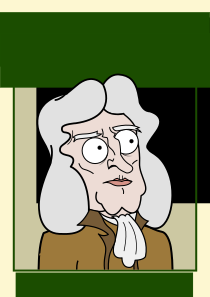
\includepdf{./images/cover/cover-front}

\begin{center}

    \begin{Huge}
    \textbf{Súper libro de Física}
    \end{Huge}

    \vspace{1cm}
    \textbf{Primera edición v0.1}
    \vspace{2cm}

    \begin{Large}
        Malvicino, Maximiliano R. \\
        Bosio, Federico A.
    \end{Large}

\end{center}

\clearpage
\noindent
\textbf{Prefacio}

La versión digital más reciente de este texto es gratis y puede ser descargada de
\begin{center}
    \small
    \url{https://github.com/mrmalvicino/physics-book}
\end{center}

\renewcommand{\spanishappendixname}{Anexo}
\tableofcontents

\mainmatter
\pagenumbering{arabic}


\chapter{Cinemática}

\emph{La cinemática es el estudio del movimiento.}
El movimiento suele describirse mediante tres magnitudes: posición, velocidad y aceleración.
A grandes rasgos, estas magnitudes se comprenden como sigue.
\begin{itemize}
    \item La posición indica dónde está lo que se mueve.
    \item La velocidad indica qué tan rápido se mueve.
    \item La aceleración indica con qué fuerza se mueve.
\end{itemize}

\begin{mdframed}[style=MyFrame2]
    \begin{example}
        \label{eg:mag}
    \end{example}
    \cusTi{Magnitudes cinemáticas}

    Para un auto en el kilómetro 10 de la Ruta Provincial 4, cuyo velocímetro marca \SI{60}{\kilo\meter/\hour}, y cuyo conductor pisa bruscamente el freno:
    \begin{itemize}
        \item La posición del auto se indica en el ``mojón kilométrico'' que, en este caso, está a \SI{10}{km} del lugar en el que nace la ruta.
        \item La velocidad está en los controles indicadores del auto, es decir, el velocímetro, que marca \SI{60}{\kilo\meter/\hour}.
        \item La aceleración está relacionada con la fuerza que sienten los pasajeros del auto cuando el conductor pisa el freno.
        La aceleración de frenado de un automóvil común ronda los \SI{5}{\meter/\second\squared}.
    \end{itemize}

    \begin{center}
        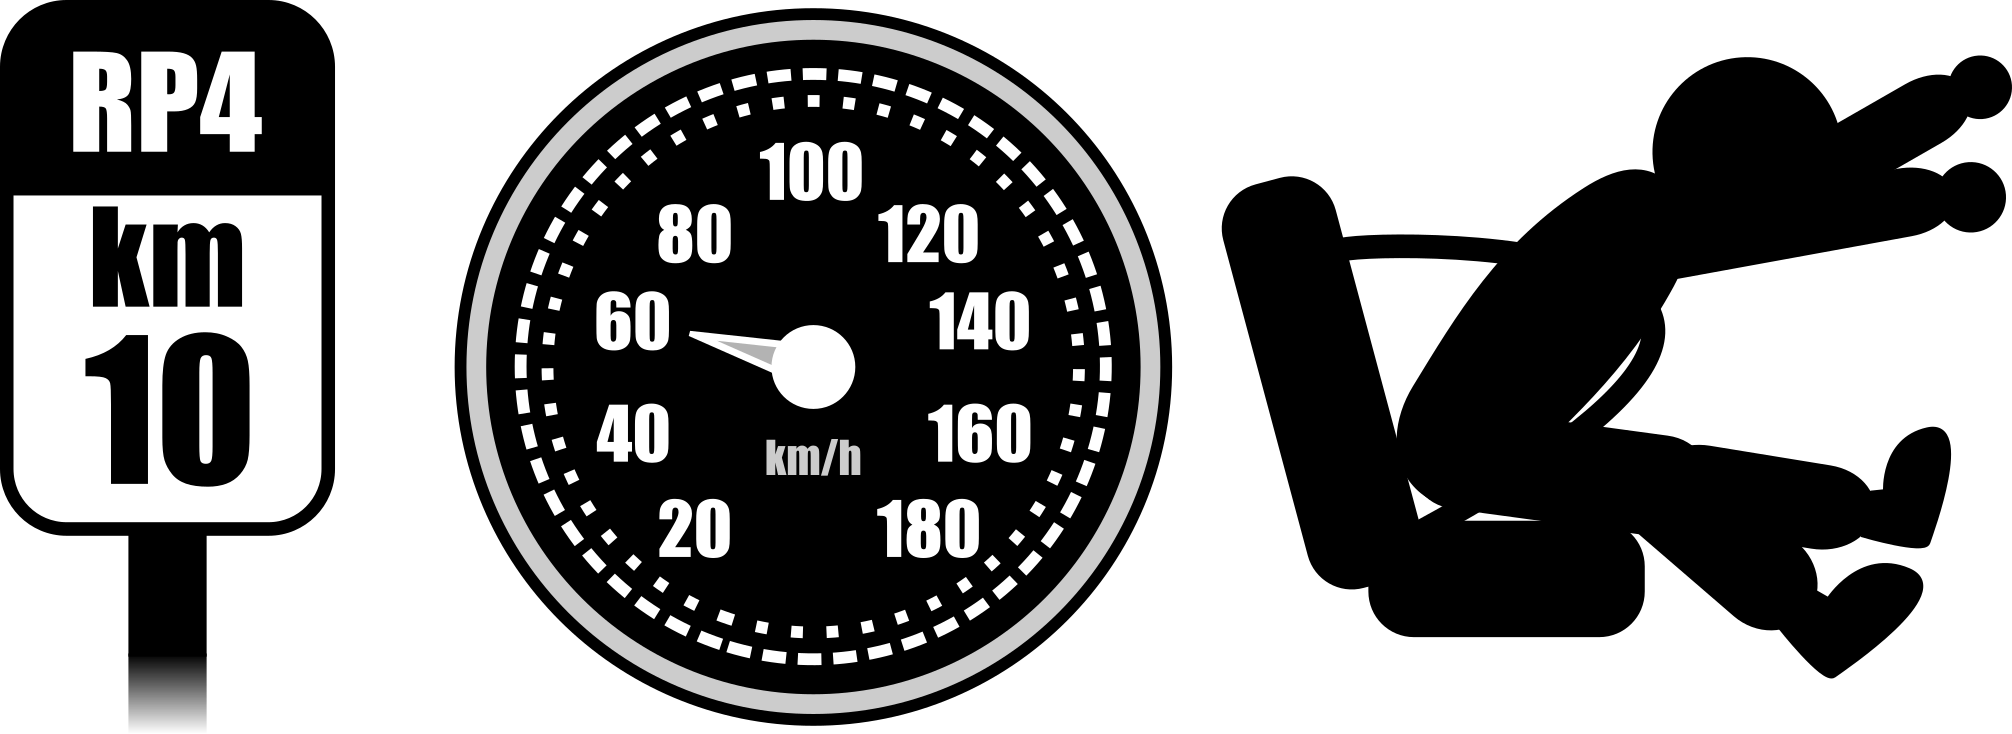
\includegraphics[width=\linewidth]{cinematica-mojon.png}
    \end{center}
\end{mdframed}

En este capítulo, van a estudiarse distintos movimientos que involucran las tres magnitudes.
Cabe destacar que sólo se estudian los movimientos en sí, y no sus causas, que se verán en capítulos posteriores.

\section{Posición, trayectoria y desplazamiento}

La posición se modela matemáticamente como un vector en el espacio, cuyas coordenadas se expresan en un sistema de referencia determinado.
En su forma más general, el vector posición se define como sigue.

\begin{mdframed}[style=MyFrame1]
    \begin{defn}
        \label{defn:position}
    \end{defn}
    \cusTi{Función de posición}
    \begin{equation*}
        \xyz(t) = \begin{bmatrix} x(t) & y(t) & z(t) \end{bmatrix}
    \end{equation*}
\end{mdframed}

Todas las coordenadas son funciones del tiempo, lo cual se pone de manifiesto en las $t$ entre paréntesis que aparecen en la notación.
Las relaciones que las componentes del vector posición tienen con la variable $t$ se llaman \emph{ecuaciones horarias}, \emph{ecuaciones de movimiento}, o \emph{ecuaciones paramétricas}.

A veces es necesario usar un vector pero basta con que tenga dos de las tres dimensiones espaciales.
La posición de movimientos en dos dimensiones suele denotarse entonces como $\xyz(t)=\sqb{x(t)&y(t)}$ o lo que es lo mismo $\xyz(t)=x(t)\,\iVer + y(t)\,\jVer$ siendo $\iVer$ y $\jVer$ los versores canónicos.

En muchos casos (como en el ejemplo \ref{eg:mag} del auto en la ruta), interesa solamente la distancia a una referencia (el número escrito en el cartel) y en ves de usar un vector $\xyz(t)$ se trabaja con un escalar, generalmente denotado $x(t)$.

Podemos referirnos a una única posición de un cuerpo en un instante de tiempo en particular.
Esto es, evaluar dicho instante $t_\ith$ en $\xyz(t)$ para obtener un vector que tiene valores numéricos fijos en sus componentes.

O bien podemos referirnos a todo el recorrido, dado por la imagen de $\xyz(t)$ que traza las sucesivas posiciones por las que pasa el cuerpo conforme transcurre el tiempo.
A este recorrido se lo llama \emph{trayectoria}.
La trayectoria es el espacio geométrico que ocupan todas las posiciones de un cuerpo en movimiento, dadas por $\xyz(t)$.

En el siguiente gráfico se observa que una \emph{trayectoria} es el conjunto de posiciones sucesivas por las que pasa un cuerpo, mientras que $P_{t_\ith}=\sqb{x(t_\ith)&y(t_\ith)}$ es una de las posiciones que toma el cuerpo a lo largo de su trayectoria.

\begin{center}
    \def\svgwidth{\linewidth}
    \input{./images/cinematica-trayect-1.pdf_tex}
\end{center}  

Para toda trayectoria o fragmento de trayectoria se puede definir el desplazamiento, que es el vector que une el punto inicial con el final.
Esto es, la resta entre ambos vectores:

\begin{mdframed}[style=MyFrame1]
    \begin{defn}
        \label{defn:desplazamiento}
    \end{defn}
    \cusTi{Desplazamiento}
    \begin{equation*}
        \Delta \xyz = \xyz(t_F) - \xyz(t_0)
    \end{equation*}
\end{mdframed}

El desplazamiento no debe confundirse con el largo del trayecto recorrido.
A continuación se muestran, sobre el gráfico anterior, el vector desplazamiento y el segmento de trayecto considerado en negro oscuro.
El segmento estudiado está dado arbitrariamente según se definan los puntos inicial y final.

\begin{center}
    \def\svgwidth{\linewidth}
    \input{./images/cinematica-trayect-2.pdf_tex}
\end{center}

Hay movimientos en dos dimensiones como el tiro oblicuo~(Sec. \ref{subsec:parabolicMotion}) y el movimiento circular~(Sec. \ref{sec:circularMotion}).
Estas trayectorias tienen una forma particular y serán estudiadas con más detalle posteriormente.
Pero también pueden darse otras menos comunes.

A continuación se muestra un ejemplo de una trayectoria curva que representa el recorrido de un bote en una laguna, visto desde el cielo.

\begin{mdframed}[style=MyFrame2]
    \begin{example}
        \label{eg:boatPosition}
    \end{example}
    \cusTi{Bote en una laguna: Posición}
    \begin{formatI}
        A partir de la siguiente función de posición, describir cualitativamente el movimieto.
    \end{formatI}
    \begin{equation*}
        \xyz:D \subseteq \setR \longrightarrow \setR^2 \tq \xyz(t) = \sqb{t^3\,\si{\metre\per\second^3}, t^2\,\si{\metre\per\second^2}}
    \end{equation*}

    \begin{center}
        \def\svgwidth{\linewidth}
        \input{./images/cinematica-boat-1.pdf_tex}
    \end{center}

Observar que:
    \begin{enumerate}
        \item El vector posición tiene en cada coordenada una función escalar de $t$.
        En este caso, las ecuaciones horarias son $x(t) = t^3\,\si{\metre\per\second^3}$ e $y(t) = t^2\,\si{\metre\per\second^2}$.
        \item La trayectoria curva se da en horizontal sobre la superficie de la tierra, pero una trayectoria en 2~dimensiones puede darse verticalmente, como por ejemplo una hormiga caminando en una pared o una pelota lanzada en diagonal hacia arriba.
        \item Se puede comprobar que, dependiendo de qué valor de tiempo asignemos a la función, obtendremos las coordenadas del bote.
        Las coordenadas indican la posición del bote en la laguna en diferentes instantes de tiempo.
    \end{enumerate}

    Supongamos que el tiempo negativo es el pasado y el tiempo positivo, el futuro, y que el muelle $A$ se encuentra en la coordenada $[x,y] = [-8,4]\,\si{\metre}$ y el muelle $C$ en la coordenada $[x,y] = [8,4]\,\si{\metre}$.
    Entonces deducimos que el bote partió del muelle $A$, se encuentra en el muelle $B$ y se dirige hacia el muelle $C$.
    El muelle $B$ se encuentra en el origen de coordenadas porque, si allí está el bote en el presente, entonces $t = \SI{0}{\minute}$ y, cuando el tiempo toma este valor, se tiene que $\xyz(\SI{0}{\minute}) = [0,0]\,\si{\metre}$.
    Además, concluimos que el bote tardará 4~minutos en hacer todo el recorrido, porque hace 2~minutos estaba en el muelle $A$, pues $\xyz(\SI{-2}{\minute}) = [-8,4]\,\si{\metre}$, y dentro de 2 minutos estará en el muelle $C$, pues $\xyz(\SI{2}{\minute}) = [8,4]\,\si{\metre}$.
\end{mdframed}

Cabe mencionar que la función vectorial ($\xyz$) del ejemplo anterior es inyectiva, ya que cada coordenada $[x,y]$ se obtiene a partir de un único valor del dominio $(t)$.
Una función vectorial no inyectiva pasa dos veces por el mismo lugar, es decir, en dos instantes distintos de tiempo se obtiene el mismo vector de posición.
Si estás pensando en que hay dos valores de $x$ que tienen una misma coordenada $y$ entonces no te estás dando cuenta que tanto $x$ como $y$ son valores de la imagen de la función.


\section{Velocidad y aceleración}

El cambio en la posición va a ir forjando el ``recorrido'' que haga el cuerpo.

Intuitivamente, podemos entender a la velocidad como qué tan rápido cambia la posición de un cuerpo y, análogamente, la aceleración como qué tan rápido cambia su velocidad.

La velocidad media es la razón de cambio promedio de la posición con respecto del tiempo transcurrido.

\begin{mdframed}[style=MyFrame1]
    \begin{defn}
    \end{defn}
    \cusTi{Velocidad media}
    \begin{equation*}
        \media{\Vec{v}}{\left[ t_0 ; t_1 \right]}
      = \dfrac{\Delta \xyz(t)}{\Delta t}
      = \dfrac{\xyz(t_1)-\xyz(t_0)}{t_1-t_0}
    \end{equation*}
\end{mdframed}

Y la aceleración media es la razón de cambio promedio de la velocidad con respecto del tiempo.

\begin{mdframed}[style=MyFrame1]
    \begin{defn}
    \end{defn}
    \cusTi{Aceleración media}
    \begin{equation*}
        \media{\Vec{a}}{\left[ t_0 ; t_1 \right]}
      = \dfrac{\Delta \Vec{v}(t)}{\Delta t}
      = \dfrac{\Vec{v}(t_1)-\Vec{v}(t_0)}{t_1-t_0}
    \end{equation*}
\end{mdframed}

La velocidad y aceleración \emph{media} se diferencian de la velocidad y aceleración \emph{instantánea}, respectivamente, en la forma que lo hacemos a continuación.

Hacer un análisis \emph{instante a instante} significa \emph{estudiar intervalos de tiempo infinitamente cortos}.
Es decir, ya que consideramos el tiempo continuo, entre dos instantes de tiempo determinados hay infinitos instantes que los separan.
La aplicación matemática que nos permite hacer este análisis es el límite
Aplicando límite en las definiciones anteriores podemos observar que quedan definidas las derivadas.
Coloquialmente, decimos que los $\Delta$ pasan a ser $\dif$.

En Cinemática, la ventaja de trabajar con funciones vectoriales es que derivarlas es muy fácil, ya que se derivan componente a componente:
\[
  \xyz (t) = \begin{bmatrix} x(t) & y(t) \end{bmatrix} \implies
  \dfrac{\dif}{\dif t} \xyz (t) =
  \begin{bmatrix} \dfrac{\dif}{\dif t} x(t) & \dfrac{\dif}{\dif t} y(t) \end{bmatrix}
\]

Por lo tanto, la velocidad está definida como la primera derivada de la posición.
\begin{equation*}
    \Vec{v}\left(t_0\right) = \lim_{t \to t_0} \dfrac{\xyz(t)-\xyz(t_0)}{t-t_0}
\end{equation*}

\begin{mdframed}[style=MyFrame1]
    \begin{defn}
    \end{defn}
    \cusTi{Velocidad (instantánea)}
    \begin{equation*}
        \Vec{v}(t) = \dfrac{\dif}{\dif t} \xyz (t) = \sqb{\dfrac{\dif}{\dif t} x(t) & \dfrac{\dif}{\dif t} y(t)}
    \end{equation*}
\end{mdframed}

Y la aceleración está dada por la primera derivada de la velocidad, o lo que es lo mismo, por la segunda derivada de la posición.
\begin{gather*}
    \Vec{a}\left(t_0\right) = \lim_{t \to t_0} \dfrac{\Vec{v}(t)-\Vec{v}(t_0)}{t-t_0}
    \\
    \Vec{a}(t) =
    \dfrac{\dif}{\dif t} \Vec{v} (t) =
    \dfrac{\dif}{\dif t} \underbrace{\dfrac{\dif}{\dif t} \xyz (t)}_{\Vec{v}(t)}
\end{gather*}

\begin{mdframed}[style=MyFrame1]
    \begin{defn}
    \end{defn}
    \cusTi{Aceleración (instantánea)}
    \begin{equation*}
        \Vec{a}(t) =
        \dfrac{\dif^2}{\dif t^2} \xyz (t) =
        \begin{bmatrix}
            \dfrac{\dif^2}{\dif t^2} x(t) & \dfrac{\dif^2}{\dif t^2} y(t)
        \end{bmatrix}
    \end{equation*}
\end{mdframed}

Para referirse a la velocidad instante a instante, o a la aceleración instante a instante, la palabra ``instantánea'' suele darse por sobreentendida.

\begin{mdframed}[style=MyFrame2]
    \begin{example}
    \end{example}
    \cusTi{Bote en una laguna: Velocidad y aceleración.}
    \begin{formatI}
        Calcular la velocidad y la aceleración a partir de la trayectoria propuesta en el ejemplo \ref{eg:boatPosition}.
    \end{formatI}
    La posición está dada por:
    \begin{equation*}
        \xyz(t) = \sqb{t^3\,\si{\metre\per\second^3}, t^2\,\si{\metre\per\second^2}}
    \end{equation*}

    Haciendo la primera derivada de la trayectoria obtenemos la velocidad:
    \[ \Vec{v}(t) = \sqb{3\,t^2\,\si{\metre\per\second^3}, 2\,t\,\si{\metre\per\second^2}} \]

    Obsérvese que $\Vec{v}(0\,\si{\second}) = [0, 0]\,\si{\metre\per\second}$.
    La velocidad en el origen es nula.
    El bote \emph{frena} para invertir el sentido del movimiento: primero va hacia el sur desde el muelle $A$ hasta el muelle $B$ y luego hacia el norte para llegar al muelle $C$.
    Esto sólo puede lograrse frenando en medio del movimiento.

    Haciendo la segunda derivada de la posición, que es la derivada de la velocidad, obtenemos la aceleración:
    \[ \Vec{a}(t) = \sqb{6\,t\,\si{\metre\per\second^3}, 2\,\si{\metre\per\second^2}} \]

    El hecho de que la aceleración tenga una componente $y$ constante indica la tendencia del bote a cambiar la dirección de su velocidad para que apunte en la dirección positiva del eje $y$.
    Esto es absolutamente consistente con el comportamiento de la velocidad.
    \begin{align*}
        \Vec{v} \left(-2\,\si{\second}\right)
        &= \sqb{3 \left(-2\,\si{\second}\right)^2\,\si{\metre\per\second^3}, 2\left(-2\,\si{\second}\right)\,\si{\metre\per\second^2}}
        \\
        &= \sqb{12, -4}\,\si{\metre\per\second}
        \\[1ex]
        \Vec{v} \left(2\,\si{\second}\right)
        &= \sqb{3 \left(2\,\si{\second}\right)^2\,\si{\metre\per\second^3}, 2 \left(2\,\si{\second}\right)\,\si{\metre\per\second^2}}
        \\
        &= \sqb{12, 4}\,\si{\metre\per\second}
    \end{align*}

    Los resultados lo muestran claramente: la velocidad del bote en el muelle $A$ apunta en dirección de las $y$ negativas (sur) y, en el muelle $C$, en dirección de las positivas (norte).
    Es precisamente la aceleración positiva en $y$ la que produjo este cambio.
\end{mdframed}


\section{Ecuación de movimiento}

Anteriormente se mencionó que la aceleración es la derivada de la velocidad, que a su vez es la derivada de la posición.
En otras palabras, se puede calcular la aceleración a partir de la posición.
De manera inversa, se puede deducir la posición o ecuación de movimiento a partir de las definiciones de velocidad y aceleración:
\[
  \left\{
   \begin{aligned}
    v &= \dfrac{\dif x}{\dif t}
    \\[1ex]
    a &= \dfrac{\dif^2 x}{\dif t^2} =
    \dfrac{\dif}{\dif t} \dfrac{\dif x}{\dif t} =
    \dfrac{\dif v}{\dif t}
   \end{aligned}
  \right.
\]

Coloquialmente, podemos pensar que los $\dif t$ pasan multiplicando al otro miembro en cada ecuación.
Formalmente, estamos calculando el diferencial de distancia $\dif x$ y el diferencial de velocidad $\dif v$, que son aproximaciones lineales de $\Delta x$ y $\Delta v$ respectivamente:
\[
  \left\{
    \begin{aligned}
    v \, \dif t &= \dif x
    \\
    a \, \dif t &= \dif v
    \end{aligned}
  \right.
\]

Ahora, integramos respecto de $t$ entre $t_0$ y $t_1$, tomando a $x$ y $v$ como funciones de $t$.
\[
  \left\{
   \begin{aligned}
     \displaystyle\int_{t_0}^{t_1} v \, \dif t &= \displaystyle\int_{x_0}^{x_1} \dif x =
     \left( x \Big|_{x_0}^{x_1} \right) = x_1 - x_0
     \\[1ex]
     \displaystyle\int_{t_0}^{t_1} a \, \dif t &= \displaystyle\int_{v_0}^{v_1} \dif v =
     \left( v \Big|_{v_0}^{v_1} \right) = v_1 - v_0
   \end{aligned}
  \right.
\]
Observar que $x_0$ es la imagen de $x(t_0)$, $x_1$ es la imagen de $x(t_1)$, $v_0$ es la imagen de $v(t_0)$, $v_1$ es la imagen de $v(t_1)$ y $t_1$ puede ser cualquier valor de $t$ mayor que $t_0$.

Haciendo algunos movimientos algebraicos, se tiene:
\[
  \left\{
    \begin{aligned}
    x_1 &= \displaystyle\int_{t_0}^{t_1} v \, \dif t + x_0
    \\[1ex]
    v_1 &= \displaystyle\int_{t_0}^{t_1} a \, \dif t + v_0
    \end{aligned}
  \right.
\]
Como $t_1$ es arbitrario, puede cambiarse por un $t$ genérico, en cuyo caso $x_1$ y $v_1$ pasan a ser, respectivamente, $x$ y $v$, también genéricos.
A su vez, $v$ puede ser expresado como $v(t)$ y $a$ puede ser expresado como $a(t)$.
Esto requiere, no obstante, cambiar las variables de integración para que no coincidan con el extremo superior de las integrales definidas.
Llamemos $u$, por ejemplo, a las variables de integración.
\[
  \left\{
    \begin{aligned}
    x(t) &= \displaystyle\int_{t_0}^{t} v(u) \, \dif u + x_0
    \\[1ex]
    v(t) &= \displaystyle\int_{t_0}^{t} a(u) \, \dif u + v_0
    \end{aligned}
  \right.
\]
Pero las integrales definidas bien pueden ser expresadas como indefinidas, donde $x_0 = x\left(t_0\right)$ y $v_0 = v\left(t_0\right)$ son las constantes de integración, como se mencionó.
\[
  \left\{
    \begin{aligned}
      x(t) &= \displaystyle\int v(t) \, \dif t + x(t_0)
      \\[1ex]
      v(t) &= \displaystyle\int a(t) \, \dif t + v(t_0)
    \end{aligned}
  \right.
\]

Reemplazando $v(t)$ en $x(t)$, por sustitución se tiene:
\[ x(t) = \int \left( \int a(t) \, \dif t + v(t_0) \right) \dif t + x(t_0) \]

Esta ecuación significa que si se conoce la aceleración, la velocidad inicial, y la posición inicial de una partícula, se pueden predecir sus futuras posiciones y velocidades:
\[ x(t) = \iint a(t) \, \dif t^2 + \int v(t_0) \, \dif t + x(t_0) \]

\begin{mdframed}[style=MyFrame1]
    \begin{defn}
        \label{defn:generalMovementEqn}
    \end{defn}
    \cusTi{Ecuación general de movimiento}
    \begin{equation*}
        x(t) = \displaystyle\iint a(t) \, \dif t^2 + v(t_0) (t-t_0)   + x(t_0)
    \end{equation*}
\end{mdframed}

En Cinemática se suele analizar los movimientos de más de una dimensión componente a componente.
Por este motivo, conviene quedarnos solo con el caso particular de 1 dimensión (Def. \ref{defn:generalMovementEqn}).

Pero podemos extrapolar $x(t)$ para $n$ dimensiones, particularmente las 3 dimensiones espaciales.
El modelado se haría con la siguiente función vectorial que describe la trayectoria de una partícula en el espacio:
\[
  \xyz(t) :
  \left\{
    \begin{aligned}
      x(t) &= \displaystyle\iint a_x(t) \, \dif t^2 + \displaystyle\int v_x(t_0) \, \dif t + x(t_0)
      \\[1ex]
      y(t) &= \displaystyle\iint a_y(t) \, \dif t^2 + \displaystyle\int v_y(t_0) \, \dif t + y(t_0)
      \\[1ex]
      z(t) &= \displaystyle\iint a_z(t) \, \dif t^2 + \displaystyle\int v_z(t_0) \, \dif t + z(t_0)
    \end{aligned}
  \right.
\]

Donde cada una de las funciones escalares $x(t)$, $y(t)$ y $z(t)$ son las componentes del vector posición (Def. \ref{defn:position}).

Podemos definir dos casos particulares usados frecuentemente.
Por un lado, el caso en que la aceleración de la partícula es constante para todos los valores de tiempo que se estén integrando entre $t_0$ y $t_1$.
Y por otro lado, el caso en que la velocidad también lo es y la aceleración, además, es nula.
De esta forma, se tienen las siguientes definiciones, respectivamente:

\begin{mdframed}[style=MyFrame1]
    \begin{defn}
        \label{defn:cstAccelMovementEqn}
    \end{defn}
    \cusTi{Ec. de movimiento con aceleración constante no nula}
    \begin{equation*}
        x(t) = \dfrac{a}{2}(t-t_0)^2 + v_0(t-t_0) + x_0
    \end{equation*}
\end{mdframed}

\begin{mdframed}[style=MyFrame1]
    \begin{defn}
        \label{defn:cstVelMovementEqn}
    \end{defn}
    \cusTi{Ec. de movimiento con velocidad constante}
    \begin{equation*}
        x(t) = v_0(t-t_0) + x_0
    \end{equation*}
\end{mdframed}


\section{Movimiento rectilíneo}

Se llama así a todo movimiento unidimensional.
Su ecuación está dada por la definición \ref{defn:generalMovementEqn}, que involucra únicamente una función escalar.

\subsection{MRU}

Un cuerpo en movimiento rectilíneo uniforme (o MRU) es aquel que se mueve en línea recta con aceleración nula, y por lo tanto con velocidad constante.

La ecuación de movimiento con velocidad constante (Def.\ \ref{defn:cstVelMovementEqn}) describe la trayectoria de un MRU.

Por ahora, si el lector quiere verificar que si la aceleración es nula entonces la velocidad será constante, puede hacerlo derivando dos veces la trayectoria del MRU.
Más adelante, en el capítulo \ref{cha:dinamics}, se enunciará la primera ley de Newton (Def.\ \ref{defn:NewtonFirstLaw}) que generaliza esta situación.

\begin{mdframed}[style=MyFrame2]
    \begin{example}
    \end{example}
    \cusTi{Auto en la ruta a velocidad constante}
    \begin{formatI}
        Un auto conduce un segmento de \SI{2,2}{\kilo\meter} de la ruta~40 en la provincia de Mendoza, entre las calles Araóz y Boedo, donde la ruta es prácticamente recta.
        El conductor parte del cruce entre la ruta 40 y Boedo y quiere saber a qué velocidad $(v)$ tiene que configurar el piloto automático para hacer la segunda mitad del trayecto, hasta Araóz, en un minuto.
    \end{formatI}
    
    \begin{center}
        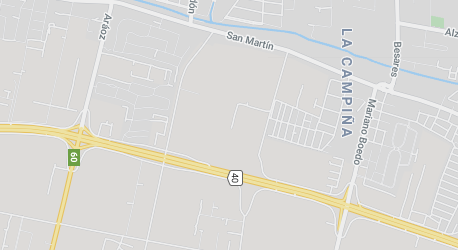
\includegraphics[width=\linewidth]{cinematica-map.png}
    \end{center}
    
    \begin{align*}
        x\left(\SI{60}{\second}\right) &= v \, \SI{60}{\second} + \SI{1100}{\metre} = \SI{2200}{\metre}
        \\[1ex]
        v &= \dfrac{\SI{2200}{\metre}-\SI{1100}{\metre}}{\SI{60}{\second}}
        = \dfrac{\SI{1100}{\metre}}{\SI{60}{\second}}
        = \dfrac{\SI{55}{\metre}}{\SI{3}{\second}}
        \\[1ex]
        &= \dfrac{55 \cdot \frac{1}{1000}\si{\kilo\meter}}{3 \cdot \frac{1}{3600}\si{\hour}}
        = \SI{66}{\kilo\metre/\hour}
    \end{align*}
    
    El sistema de referencia está planteado para que la función de posición tenga origen en el comienzo del segmento de la ruta, es decir, en el cruce de la ruta 40 con Boedo.
    
    \begin{center}
        \def\svgwidth{\linewidth}
        \input{./images/cinematica-map-2.pdf_tex}
    \end{center}
    
    Sería posible resolver el problema, de manera más sencilla (aunque menos general) estableciendo el origen en el medio del segmento de ruta y en este caso la posición inicial sería \SI{0}{\metre} y la posición final $(x_1)$ sería \SI{1100}{\metre}.
    
    El mapa 2 tiene dimensiones, pero como el movimiento se da en línea recta, basta con una coordenada para calcular la trayectoria.
    Sería innecesario y engorroso (aunque posible) plantear una trayectoria recta de 2 dimensiones para describir el movimiento en el plano $xy$.
    Cualquier movimiento, en particular uno rectilíneo, puede expresarse con una trayectoria vectorial de 3 dimensiones.
    Pero si se elige correctamente el sistema de referencia, basta con usar 1 dimensión, porque lo que importa es la variación de la distancia.
\end{mdframed}

\begin{mdframed}[style=MyFrame2]
    \begin{example}
    \end{example}
    \cusTi{Dos autos en sentido opuesto}
    \begin{formatI}
        Para este problema de \emph{encuentro}, determinar cuándo y dónde se cruzan los móviles del siguiente esquema.
    \end{formatI}
    
    \begin{center}
        \def\svgwidth{\linewidth}
        \input{./images/cinematica-cars-1.pdf_tex}
    \end{center}
    
    En particular, acá se tienen dos autos en sus respectivos carriles y sentidos opuestos entre sí, separados por una distancia de \SI{300}{\kilo\meter}.
    Uno tiene una velocidad de \SI{50}{\kilo\meter/\hour} y el otro, de \SI{100}{\kilo\meter/\hour}.
    Se busca, como todo problema de encuentro, el instante de tiempo y la posición en que se cruzan.
    
    Tomemos el siguiente sistema de referencia.
    
    \begin{center}
        \def\svgwidth{\linewidth}
        \input{./images/cinematica-cars-2.pdf_tex}
    \end{center}
    
    El origen ($O$) coincide con la posición inicial del auto ubicado en la parte superior del dibujo ($A$).
    De acuerdo al sistema elegido, la posición crece positivamente cuando nos alejamos de $O$ para ir a la posición inicial del auto en el carril inferior ($B$).
    Además, por simplicidad, elegiremos $t_0 = 0$ en el punto $O$, es decir, el inicio del movimiento sucederá cuando el auto A esté ubicado en el punto $O$ del eje $x$.
    
    Con esto ya podemos construir las ecuaciones de movimiento.
    Si adjuntamos a cada $x$ un subíndice correspondiente a cada auto ($A$ o $B$), quedan
    \begin{align*}
        x_A(t) &= 50\,\si{\kilo\metre\per\hour} \, t
        \\
        x_B(t) &= 300\,\si{\kilo\metre} - 100\,\si{\kilo\metre\per\hour} \, t
    \end{align*}
    
    Los signos de las velocidades respetan el sentido de crecimiento del eje $x$: la velocidad de $A$ es positiva porque apunta, en el dibujo, hacia la derecha (como el eje $x$), y la velocidad de B es negativa porque apunta hacia la izquierda (contrario al eje $x$).
    
    Recordemos que, en el instante en que los autos se cruzan, están en la misma posición (en lo que respecta al eje $x$).
    Por eso basta con igualar $x_A$ y $x_B$:
    \[ 50\,\si{\kilo\metre\per\hour} \, t = 300\,\si{\kilo\metre} - 100\,\si{\kilo\metre\per\hour} \, t \]
    
    y ahora sencillamente despejamos $t$
    \[ 150\,\si{\kilo\metre\per\hour} \, t = 300\,\si{\kilo\metre}
    \iff t = \frac{300}{150}\,\si{\hour} = 2\,\si{\hour} \]
    
    Reemplazando en cualquiera de las dos ecuaciones de movimiento, queda
    \[ x_A(2\,\si{\hour}) = 100\,\si{\kilo\metre} = x_B(2\,\si{\hour}) \]
    es decir, los autos se cruzan a las \SI{2}{\hour} de haber iniciado el recorrido, \SI{100}{\kilo\meter} a la derecha del origen.
\end{mdframed}


\subsection{MRUV}

Un cuerpo en movimiento rectilíneo uniformemente variado es aquel que se mueve en línea recta con aceleración constante no nula.

La ecuación de movimiento con aceleración constante (Def. \ref{defn:cstAccelMovementEqn}) describe la trayectoria de los MRUV.

Dependiendo de la naturaleza de la aceleración, podemos distinguir los movimientos dados por la aceleración gravitatoria de los que son acelerados de manera arbitraria por un agente externo.

La diferencia entre los MRUV con aceleración gravitatoria $(g)$ y aquellos con aceleración arbitraria $(a)$ es que $g$ tiene un valor predefinido y conocido mientras que $a$ puede tomar un valor diferente dependiendo de cada situación.

\begin{itemize}
    \item
    El efecto de la gravedad a escala visible es evidente: si dejo caer un objeto desde cierta altura, su velocidad aumenta cada vez más, lo cual significa que el objeto está acelerado.
    La aceleración de una partícula debido al campo gravitatorio de la Tierra vale $a = g \approx \SI{9,8}{\metre/\second\squared}$.

    \item
    El efecto de un agente externo acelerando un cuerpo (como, por ejemplo, un motor acelerando un auto) no es tan trivial.
    A continuación se dan algunos ejemplos aunque más adelante, para hacer un estudio más exhaustivo, se enunciará la segunda ley de Newton (Def.\ \ref{defn:NewtonSecondLaw}) que permite dar otro enfoque.
\end{itemize}

\begin{mdframed}[style=MyFrame2]
    \begin{example}
    \end{example}
    \cusTi{Auto en la ruta con aceleración constante}
    \begin{formatI}
        Calcular el tiempo que tarda un auto en acelerar de \SI{0}{\kilo\meter\per\hour} a \SI{100}{\kilo\meter\per\hour} si tiene una aceleración $(a)$ de $\num{0,3}\,g$ a lo largo de una ruta recta.
        Luego, calcular la longitud $(L)$ del segmento de ruta que recorrió en ese tiempo.
    \end{formatI}
    \begin{gather*}
        a = \num{0,3}\,g = \num{0,3} \left( \SI{9,8}{\metre\per\second\squared} \right) = \SI{2,94}{\metre\per\second\squared}
        \\[1ex]
        v(t_1) = \SI{2,94}{\metre\per\second\squared} \, t_1
        \\
        v(t_1) = \SI{100}{\kilo\metre\per\hour}
        = \dfrac{250}{9} \, \si{\metre\per\second}
        \\[1ex]
        t_1 = \dfrac{\frac{250}{9} \, \si{\metre\per\second}}{\SI{2,94}{\metre\per\second\squared}}
        \approx \SI{9,4}{\metre\second\squared\per\metre\per\second}
        = \SI{9,4}{\second}
        \\[1ex]
        x(t_1) =  \frac{a}{2} \, t_1^2 + v_0 \, t_1 + x_0  =  L
        \\
        L =  \dfrac{\SI{2,94}{\metre\per\second\squared}}{2}t_1^2 \approx \SI{130}{\metre}
    \end{gather*}
\end{mdframed}

\begin{mdframed}[style=MyFrame2]
    \begin{example}
    \end{example}
    \cusTi{Nave espacial despegando}
    \begin{formatI}
        Una nave espacial mantiene una aceleración de $\num{1,8}\,g$ desde su despegue hasta que sale de la atmósfera terrestre después de 10 minutos.
        Verificar que la velocidad que tiene la nave al finalizar ese trayecto, es menor a la velocidad máxima del Falcon 9 Heavy de SpaceX, la cual se estima en~\SI{39600}{\kilo\metre/\hour}.
    \end{formatI}
    \begin{align*}
        a &= \num{1,8}\,g = 17,64 \, \si{\metre\per\second\squared} \implies
        \\
        v \left(\SI{600}{\second}\right) &= \left(\SI{17,64}{\metre\per\second\squared}\right) \SI{600}{\second}
        \\
        &= \SI{10584}{\metre\per\second}
        \\
        &= \SI{38102,4}{\kilo\metre\per\hour} < \SI{39600}{\kilo\metre\per\hour}
    \end{align*}
\end{mdframed}


\subsection{Caída libre}

En esta situación, un cuerpo puntual cae desde cierta altura $(h)$, medida desde el piso, y adquiere una aceleración de magnitud $g$ y sentido hacia abajo.
Tanto el movimiento como la aceleración son hacia abajo.
Esto no es menor, y se tiene que ver reflejado en la ecuación, de acuerdo al sistema de referencia que se tome.

La caída libre es un tipo de MRUV, por lo que la trayectoria va a ser modelada por la ecuación de movimiento con aceleración constante (Def.\ \ref{defn:cstAccelMovementEqn}) tomando las siguientes consideraciones.

Como el cuerpo parte del reposo, la velocidad inicial es $v_0 = \SI{0}{\metre/\second}$.
Si elegimos un sistema orientado positivamente hacia arriba y con el origen en el piso, la posición inicial $\left( x_0 \right)$ va a ser igual a $h$ y la aceleración $(a)$ va a ser negativa:

\begin{mdframed}[style=MyFrame1]
    \begin{defn}
    \end{defn}
    \cusTi{Función de posición de caída libre}
    \begin{equation*}
        y(t) = -\frac{g}{2} \left(t-t_0\right)^2 + h
    \end{equation*}
\end{mdframed}


\subsection{Tiro vertical}

En esta situación un cuerpo puntual cae desde cierta altura $(h)$ y adquiere aceleración gravitatoria $(g)$ con sentido hacia abajo.
Pero además, al inicio del movimiento el cuerpo tiene una velocidad inicial $(v_0)$.

Al igual que la caída libre, el tiro vertical se modela con la ecuación de movimiento con aceleración constante (Def.\ \ref{defn:cstAccelMovementEqn}), ya que también es un caso particular de MRUV.

Ahora bien, en este caso se va a mantener el término lineal para incorporar el dato de la velocidad inicial, siendo su signo positivo si, al inicio del movimiento, el cuerpo estaba subiendo, y negativo si estaba bajando.

\begin{mdframed}[style=MyFrame1]
    \begin{defn}
    \end{defn}
    \cusTi{Función de posición del tiro vertical}
    \begin{equation*}
        y(t) = -\frac{g}{2}(t-t_0)^2 \pm v_0(t-t_0) + h
    \end{equation*}
\end{mdframed}


\section{Movimiento curvilíneo}

Hasta ahora se vieron situaciones en las que se daba un movimiento que podía ser acelerado o no, pero siempre era en línea recta.
Por este motivo, usábamos la ecuación de movimiento en una dimensión (Def.\ \ref{defn:generalMovementEqn}) y sus casos particulares.
Si queremos estudiar una trayectoria curva, necesitamos una parametrización de dos dimensiones.
Esto implica que la posición, la velocidad y la aceleración van a considerarse magnitudes vectoriales, y ya no escalares.
Para estudiar un movimiento curvilíneo, hay que analizar cómo estas magnitudes son afectadas en cada dimensión, descomponiéndolas.


\section{Tiro oblicuo}
\label{subsec:parabolicMotion}

En esta situación, un cuerpo puntual es arrojado en diagonal con cierto ángulo $(\theta)$ y cierta velocidad inicial $(\Vec{v_0})$ de módulo $\nnorm{\Vec{v_0}} = v_0$.
Al descomponer el movimiento para analizar cómo va a variar la cinemática en cada dimensión, podemos observar que:
\begin{itemize}
    \item
    El eje $z$ no es necesario, ya que si despreciamos cualquier desvío causado por el viento empujando al cuerpo, el movimiento se modela sobre un plano, en dos dimensiones.
    
    \item
    La trayectoria del cuerpo se va a curvar por la gravedad.
    Pero esta aceleración solo va a afectar el eje $y$ del movimiento, como si de un tiro vertical se tratase.
    Por lo tanto, la coordenada vertical de la posición estará dada por la ecuación de movimiento con aceleración constante (Def.\ \ref{defn:cstAccelMovementEqn}).
    
    \item
    El eje $x$ no se ve afectado por aceleración alguna.
    Con lo cual, la coordenada horizontal de la posición estará dada por la ecuación de movimiento con velocidad constante (Def.\ \ref{defn:cstVelMovementEqn}).
    La velocidad en $x$ será contantemente $v_{0x}$, que es aquella impuesta inicialmente por la velocidad inicial.
\end{itemize}

A partir de este análisis, podemos definir la aceleración que rige el movimiento:
\begin{equation*}
    \Vec{a}(t) = \sqb{0 \, , \, -g}
\end{equation*}

Y así también la velocidad, que surge al integrar la aceleración:
\begin{equation*}
    \Vec{v}(t) = \sqb{v_{0x} \, , \, -g \left(t-t_0\right) + v_{0y}}
\end{equation*}

Obteniendo así la posición al integrar nuevamente.

\begin{mdframed}[style=MyFrame1]
    \begin{defn}
    \end{defn}
    \cusTi{Función de posición del tiro oblicuo}
    \begin{equation*}
        \scale{0.92}{
        \xyz(t) = \sqb{v_{0x} \left(t-t_0\right) \, , \, \frac{-g}{2} \left(t-t_0\right)^2 + v_{0y} \left(t-t_0\right) + y_0}
        }
    \end{equation*}
\end{mdframed}

Veamos la fórma que tiene el recorrido de un cuerpo arrojado en tiro oblicuo.

Como estamos estudiando un único cuerpo podemos establecer $t_0=\SI{0}{\second}$ ya que para estudiar una única trayectoria no es necesario considerar un retraso temporal.
Las coordenadas $x(t)$ e $y(t)$ del vector $\xyz(t) = \sqb{x(t),y(t)}$ quedan entonces dadas por:
\begin{equation*}
    \left\{
    \begin{aligned}
        x(t) &= v_{0x} \, t
        \\
        y(t) &= -\frac{g}{2} \, t^2 + v_{0y} \, t + y_0
    \end{aligned}
    \right.
\end{equation*}

Despejando el parámetro $t$ de la primer ecuación y reemplazándolo en la segunda, se tiene:
\begin{align}
    y &= -\frac{g}{2} \, \left(\frac{x}{v_{0x}}\right)^2 + v_{0y} \left(\frac{x}{v_{0x}}\right) + y_0
    \notag
    \\
    y(x) &= -\frac{g}{2 \, v_{0x}^2} \, x^2 + \frac{v_{0y}}{v_{0x}} \, x + y_0
    \label{eqn:oblicuoCurva}
\end{align}

Luego, es esperable que la trayectoria de la partícula sea una parábola invertida.

A continuación, se muestra un gráfico con las implicaciones geométricas en la trayectoria del movimiento.
Notar que se está graficando, en un mismo gráfico, la trayectoria y la velocidad de la partícula en ciertos puntos de la misma.
El largo de las flechas, indica la magnitud del vector.

\begin{center}
    \def\svgwidth{\linewidth}
    \input{./images/cinematica-tiro-oblicuo-1.pdf_tex}
\end{center}

Donde:
\begin{align*}
    v_{0x} &= v_0 \cos(\theta)
    \\
    v_{0y} &= v_0 \sin(\theta)
\end{align*}

Concluyendo que:

\begin{itemize}
    \item
    La componente vertical de la velocidad $(v_y)$ va disminuyendo hasta que se hace nula en el punto $\sqb{x_h, y_h}$, donde la altura es máxima y el módulo de la velocidad es mínimo (pero no nulo).
    
    \item
    El módulo de la velocidad es máximo en el punto donde la altura es mínima $(y=\SI{0}{\metre})$.
    Esto sucede al final del recorrido, justo antes de que el cuerpo choque contra el piso.
    
    \item Para todos los pares de puntos donde la altura es la misma, la velocidad tiene el mismo módulo y el vector velocidad forma el mismo ángulo con el eje $x$ pero hacia abajo.
    
    \item La componente horizontal de la velocidad $(v_x)$ es constante para todos los puntos de la trayectoria.
\end{itemize}

Cuando se estudian las posibles trayectorias de un tiro oblicuo, suele ser de interés calcular el \emph{alcance} que va a tener el cuerpo.
Esta distancia $x_d$ para la cual el cuerpo impacta en el piso está dada para el punto cuya coordenada vertical es nula.

Así, al igualar a cero la ecuación \ref{eqn:oblicuoCurva} se tiene, completando cuadrados:
\begin{align*}
    0 &= -\frac{g}{2 \, v_{0x}^2} \, x^2 + \frac{v_{0y}}{v_{0x}} \, x + y_0
    \\[1ex]
    &= x^2 - \frac{2 \, v_{0x}^2}{g} \frac{v_{0y}}{v_{0x}} \, x - \frac{2 \, v_{0x}^2}{g} \, y_0
    \\[1ex]
    &= x^2 - 2 \, \frac{v_{0x} \, v_{0y}}{g} \, x - \frac{2 \, v_{0x}^2}{g} \, y_0
    \\[1ex]
    &= \left(x - \frac{v_{0x} \, v_{0y}}{g}\right)^2 - \left(\frac{v_{0x} \, v_{0y}}{g}\right)^2 - \frac{2 \, v_{0x}^2}{g} \, y_0
\end{align*}

Entonces, si consideramos $y_0=\SI{0}{\metre}$ como un caso particular, el alcance es:
\begin{align*}
    \left(x - \frac{v_{0x} \, v_{0y}}{g}\right)^2 &= \left(\frac{v_{0x} \, v_{0y}}{g}\right)^2
    \\[1ex]
    x &= \frac{2 \, v_{0x} \, v_{0y}}{g}
    \\[1ex]
    &= \frac{2 \cos(\theta) \sin(\theta) \, v_0^2}{g}
\end{align*}

Y, finalmente, usando la propiedad trigonométrica del seno de ángulo doble que implica $2 \cos(\theta) \sin(\theta)=\sin(2\theta)$ se obtiene

\begin{mdframed}[style=MyFrame1]
    \begin{prop}
        \label{prop:oblicuoAlcance}
    \end{prop}
    \cusTi{Alcance de tiro oblicuo}
    \begin{equation*}
        y_0 = \SI{0}{\metre} \implies x_d = \frac{\sin(2\theta) \, v_0^2}{g}
    \end{equation*}
\end{mdframed}

Aunque podríamos usar las parametrizaciones $x(t)$ e $y(t)$ para dar con una fórmula para el alcance que admita $y_0 \neq \SI{0}{\metre}$.
Primero se calcula el tiempo $t=t_d$ tal que $y(t)=\SI{0}{\metre}$ siendo este lo que tarda el cuerpo en tener altura nula.
Completando cuadrados esto es:
\begin{align*}
    0 &= -\frac{g}{2} \, t^2 + v_{0y} \, t + y_0
    \\[1ex]
    &= t^2 - 2 \, \frac{v_{0y}}{g} \, t - \frac{2\,y_0}{g}
    \\[1ex]
    &= \left( t - \frac{v_{0y}}{g} \right)^2 - \left(\frac{v_{0y}}{g}\right)^2 - \frac{2\,y_0}{g}
    \\[1ex]
    \left( t - \frac{v_{0y}}{g} \right)^2 &= \left(\frac{v_{0y}}{g}\right)^2 + \frac{2\,y_0}{g}
    \\[1ex]
    t>\frac{v_{0y}}{g} \implies t_d &= \sqrt{\left(\frac{v_{0y}}{g}\right)^2 + \frac{2\,y_0}{g}} + \frac{v_{0y}}{g}
\end{align*}

Y luego se evalúa $x(t_d)$ para obtener el alcance:
\begin{align*}
    x_d &= v_{0x} \, t_d
    \\[1ex]
    &= \sqrt{v_{0x}^2} \sqrt{\left(\frac{v_{0y}}{g}\right)^2 + \frac{2\,y_0}{g}} + \frac{v_{0x}\,v_{0y}}{g}
    \\[1ex]
    &= \sqrt{\left(\frac{v_{0x}\,v_{0y}}{g}\right)^2 + \frac{2 \, y_0 \, v_{0x}^2}{g}} + \frac{v_{0x}\,v_{0y}}{g}
\end{align*}

O bien, usando trigonometría podemos expresar el resultado en función de la norma de la velocidad inicial ($v_0$) y el ángulo ($\theta$) que forma con la horizontal.
\begin{multline*}
    x_d = \sqrt{\left(\frac{v_0^2 \cos(\theta) \sin(\theta)}{g}\right)^2 + \frac{2 \, y_0 \, v_0^2 \cos^2(\theta)}{g}} +
    \\ + \frac{v_0^2 \cos(\theta) \sin(\theta)}{g}
\end{multline*}

Y, finalmente, usando la propiedad trigonométrica del seno de ángulo doble se obtiene

\begin{mdframed}[style=MyFrame1]
    \begin{prop}
    \end{prop}
    \cusTi{Alcance de tiro oblicuo}
    \begin{equation*}
        \scale{0.94}{
        x_d = \sqrt{\left(\frac{\sin(2\theta) \, v_0^2}{2g}\right)^2 + \frac{2 \, y_0 \, v_0^2 \cos^2(\theta)}{g}} + \frac{\sin(2\theta) \, v_0^2}{2g}
        }
    \end{equation*}
\end{mdframed}

A partir de cualquiera de ambas propiedades podemos estudiar el alcance en función del ángulo de tiro tomando un valor fijo para $v_0$.

Para el caso en que $y_0 = \SI{0}{\metre}$ se puede usar la propiedad \ref{prop:oblicuoAlcance} para estudiar $x_d$ en función de $\theta$ como sigue.
\begin{equation*}
    x_d = \frac{\sin(2\theta) \, v_0^2}{g}
\end{equation*}

El gráfico de la función $\sin(2\theta)$ está acotado tal que
\begin{equation*}
    0 \leq \theta \leq \ang{90} \Rightarrow 0 \leq x_d \leq \frac{v_0^2}{g}
\end{equation*}

Y presenta un máximo en $\theta=\pi/4$.
Lo cual significa que el alcance $x_d$ va a tomar un valor de $v_0^2/g$ como máximo cuando el ángulo de tiro sea $\ang{45}$.
Además, dado que las funciones senoidales son simétricas con respecto a un máximo, vemos que el alcance va a ser el mismo para ángulos simétricos con respecto de $\ang{45}$.
Esto se traduce en la siguiente propiedad.

\begin{mdframed}[style=MyFrame1]
    \begin{prop}
    \end{prop}
    Sea $\alpha>0$ el módulo de la diferencia entre $\ang{45}$ y el ángulo de tiro ($\theta$).
    Para el caso $y_0 = \SI{0}{\metre}$ de tiro oblicuo se tiene que
    \begin{equation*}
        x_d(\theta_1) = x_d(\theta_2) \iff \theta_{1,2} = \ang{45} \pm \alpha
    \end{equation*}
\end{mdframed}

A continuación podemos ver un gráfico que ilustra estas conclusiones.
En él se muestran algunas de las posibles trayectorias de un tiro oblicuo en función de una velocidad inicial con ángulo variable pero de norma constante.

\begin{center}
    \def\svgwidth{\linewidth}
    \input{./images/cinematica-tiro-oblicuo-2.pdf_tex}
\end{center}


\section{Movimiento circular}
\label{sec:circularMotion}

El movimiento circular es otro caso particular de movimiento curvilíneo.
En un movimiento curvilíneo cualquiera, un cuerpo puede tener una trayectoria errática.
En cambio, la trayectoria de un cuerpo en movimiento circular está delimitada por un círculo.

El inconveniente a la hora de deducir ecuaciones horarias para describir la posición de la partícula es que no es posible identificar un valor de aceleración constante en ninguno de los ejes cartesianos, tal como se hacía por ejemplo para un tiro verical donde se podía afirmar que $a_x=\SI{0}{\metre\per\second^2}$ y $a_y=-g\,\si{\metre\per\second^2}$.
Es por esto que es necesario usar {coordenadas polares} para referir las magnitudes a estudiar.
Ver sección \ref{A:polarCoordinates} del anexo.

A continuación, se muestra el gráfico de una trayectoria circular para una partícula, representada por un punto negro, junto con la posición y sus componentes cartesianas, la velocidad que tiene en ese punto, y las aceleraciones que pueden estar afectando el movimiento.

\begin{center}
    \def\svgwidth{\linewidth}
    \input{./images/cinematica-circular-1.pdf_tex}
\end{center}

La posición $(\xyz)$ se puede expresar como un vector que rota con un extremo fijo en el centro del círculo, como la aguja de un reloj.
Las componentes del vector cambian conforme pasa el tiempo.
Pero el largo del vector posición es siempre el mismo, y es equivalente al radio $(r)$ del círculo.

\begin{mdframed}[style=MyFrame1]
    \begin{prop}
        \label{prop:circularMovRadius}
    \end{prop}
    \cusTi{Radio del movimiento circular}
    \begin{equation*}
        r = \nnorm{\xyz(t)}
    \end{equation*}
\end{mdframed}

En un movimiento curvilíneo cualquiera, la velocidad ``neta'' puede definirse a partir de la suma entre las velocidades tangencial y radial.

\begin{mdframed}[style=MyFrame1]
    \begin{defn}
    \end{defn}
    \cusTi{Velocidad en polares}
    \begin{equation*}
        \Vec{v} = \Vec{v}_t + \Vec{v}_r
    \end{equation*}
\end{mdframed}

Además, la velocidad de un cuerpo tiene que ser tangente a su trayectoria en todo momento.
Pero no hay que confundir la naturaleza tangencial de la velocidad con respecto a la trayectoria con la componente tangencial de la velocidad, que hace referencia a la ortogonalidad entre el vector velocidad y el radio de la circunferencia que pasa por un punto de la trayectoria.
En la siguiente imagen vemos una trayectoria curvilínea cualquiera (en línea punteada) sobre la que se grafican los vectores velocidad para dos posiciones distintas.

\begin{center}
    \def\svgwidth{\linewidth}
    \input{./images/cinematica-circular-2.pdf_tex}
\end{center}

En ambos puntos la velocidad es tangencial a la trayectoria, pero solo $\vec{v}_1$ es ortogonal a la dirección radial del círculo de referencia.

La componente radial de la velocidad impone cómo tiende a darse la trayectoria hacia adentro o hacia afuera del círculo de referencia.
Si existiese una componente radial de velocidad se podría formar una trayectoria espiral, por ejemplo.

Pero $\nnorm{\Vec{v}_r} = \SI{0}{\metre\per\second}$ ya que para que la trayectoria sea circular se tiene que cumplir la siguiente propiedad.

\begin{mdframed}[style=MyFrame1]
    \begin{prop}
        \label{prop:circularMovVel}
    \end{prop}
    \cusTi{Velocidad del movimiento circular}
    \begin{equation*}
        \Vec{v} = \Vec{v}_t
    \end{equation*}
\end{mdframed}

Un cuerpo en movimiento circular está sometido a una aceleración radial $(\vec{a}_r)$ o centrípeta $(\Vec{a}_c)$ en todo momento.
Esta apunta hacia el centro y su magnitud es tal que contrarresta la tendencia ``natural'' del cuerpo a tener una trayectoria recta.
Cabe aclarar que la aceleración radial es la misma que la centrípeta: solo se diferencian por ser opuestas en su notación.

El movimiento circular puede o no tener aceleración tangencial $(\Vec{a}_ t)$.
La aceleración tangencial puede ser positiva o negativa, dependiendo de la situación.
De existir, esta hace que el cuerpo se mueva cada vez más (o menos) rápido sobre el círculo.

\begin{mdframed}[style=MyFrame1]
    \begin{defn}
    \end{defn}
    \cusTi{Aceleración en polares}
    \begin{equation*}
        \Vec{a} = \Vec{a}_t + \Vec{a}_r = \Vec{a}_t - \Vec{a}_c
    \end{equation*}
\end{mdframed}

A medida que el ángulo $(\theta)$ aumenta o disminuye en sentido horario o antihorario, la partícula se mueve por la circunferencia trazando un arco de círculo de cierto largo $(s)$.
Es evidente que para que la partícula se mueva, el ángulo va a cambiar conforme pase el tiempo.
Ergo, el ángulo es una función escalar del tiempo.

Es determinante qué tan rápido aumenta o disminuye el ángulo.
La tasa de cambio del ángulo con respecto del tiempo se conoce como velocidad angular $(\omega)$.

\begin{mdframed}[style=MyFrame1]
    \begin{defn}
        \label{defn:angularVel}
    \end{defn}
    \cusTi{Velocidad angular}
    \begin{equation*}
        \omega (t) = \dfrac{\dif}{\dif t} \theta (t)
    \end{equation*}
\end{mdframed}

Con el mismo criterio, se define la aceleración angular $(\alpha)$ como la derivada de la velocidad angular con respecto del tiempo.

\begin{mdframed}[style=MyFrame1]
    \begin{defn}
        \label{defn:angularAccel}
    \end{defn}
    \cusTi{Aceleración angular}
    \begin{equation*}
        \alpha (t) = \dfrac{\dif}{\dif t} \omega (t) = \dfrac{\dif^2}{\dif t^2} \theta (t)
    \end{equation*}
\end{mdframed}

La velocidad angular está relacionada con la velocidad tangencial, y de igual manera la aceleración angular lo está con la aceleración tangencial.
Pero no son lo mismo.
Veamos cómo se relacionan.

Dividiendo por el incremento $\Delta t$ y luego tomando el límite cuando $\Delta t \to 0$ en la definición de longitud de arco (Sec. \ref{A:arcLength}) se tiene:
\begin{align*}
    \Delta s &= \Delta \theta \, r
    \\[1ex]
    \frac{\Delta s}{\Delta t} &= \frac{\Delta \theta}{\Delta t} \, r
    \\[1ex]
    \frac{\dif s}{\dif t} &= \frac{\dif \theta}{\dif t} \, r
\end{align*}

La derivada de la izquierda es la velocidad tangencial.
Indica qué tan rápido crece el largo de arco de la circunferencia.
La derivada de la derecha es la velocidad angular.
Indica qué tan rápido aumenta el ángulo.
Se obtiene así una relación entre la velocidad angular (Def.\ \ref{defn:angularVel}) y la velocidad tangencial ($v_t$).

\begin{mdframed}[style=MyFrame1]
    \begin{prop}
        \label{prop:circularVel}
    \end{prop}
    \begin{equation*}
        v_t(t) = \omega(t) \, r
    \end{equation*}
\end{mdframed}

Derivando nuevamente, de manera similar se relaciona la aceleración angular (Def.\ \ref{defn:angularAccel}) con la tangencial ($a_t$).

\begin{mdframed}[style=MyFrame1]
    \begin{prop}
        \label{prop:circularAccel}
    \end{prop}
    \begin{equation*}
        a_t(t) = \alpha(t) \, r
    \end{equation*}
\end{mdframed}

A partir de las conclusiones anteriores, siguiendo el mismo razonamiento que se usó para definir la ecuación de movimiento (Def. \ref{defn:generalMovementEqn}), se define la variación del ángulo en función del tiempo o \emph{posición angular}.

\begin{mdframed}[style=MyFrame1]
    \begin{defn}
        \label{defn:anglePosition}
    \end{defn}
    \cusTi{Posición angular}
    \begin{equation*}
        \theta(t) = \iint \alpha(t) \, \dif t^2 + \omega (t_0) \left(t-t_0\right) + \theta(t_0)
    \end{equation*}
\end{mdframed}


\subsection{MCU}
El movimiento circular es \emph{uniforme} cuando el cuerpo gira en torno a la circunferencia con \emph{velocidad angular constante}.

El MCU hereda las propiedades \ref{prop:circularMovRadius} y \ref{prop:circularMovVel} generales para movimientos circulares.
A saber:
\begin{itemize}
    \item Al ser un movimiento circular, el radio permanece constante.
    
    \item La velocidad radial es nula y, en consecuencia, el vector velocidad sólo tiene la componente tangencial.
\end{itemize}

Además, se incorporan las siguientes propiedades particulares del MCU.

Como la velocidad angular y el radio son constantes, el módulo de la velocidad también lo es, de acuerdo a la propiedad \ref{prop:circularVel}.

\begin{mdframed}[style=MyFrame1]
    \begin{prop}
    \end{prop}
    \begin{equation*}
        v = \omega \, r
    \end{equation*}
\end{mdframed}

Velocidad angular constante implica aceleración angular cero lo cual, a su vez, implica aceleración tangencial cero (Prop.~\ref{prop:circularAccel}).

\begin{mdframed}[style=MyFrame1]
    \begin{prop}
    \end{prop}
    \cusTi{Aceleración de MCU}
    \begin{equation*}
        \Vec{a} = - a_c \, \versor{r}
    \end{equation*}
\end{mdframed}

Como $v_t = \dif s / \dif t$ por definición y, en particular, $v_t$ es constante para un MCU, entonces
\begin{align*}
    v_t \, \dif t &= \dif s
    \\[1ex]
    \int_{t_0}^{t_0+\Delta t} v_t \, \dif t &= \int_{s_0}^{s_0+\Delta s} \dif s
    \\[1ex]
    v_t \left[\left( t_0+\Delta t \right) - t_0\right] &= \left( s_0+\Delta s \right) - s_0
    \\[1ex]
    v_t \, \Delta t &= \Delta s
\end{align*}

Formalmente, integramos miembro a miembro en el intervalo de tiempo $\left[ t_0; t_0 + \Delta t \right]$.
Coloquialmente, como $v_t$ es constante, ``cambiamos los $\dif$ por $\Delta$''.

En la relación anterior, interesa particularmente el siguiente intervalo de tiempo, llamado \emph{período}.

\begin{mdframed}[style=MyFrame1]
    \begin{defn}
    \end{defn}
    \cusTi{Período}
    \cusTe{El período $(T)$ de un cuerpo en MCU es el tiempo que tarda en dar una vuelta completa.}
\end{mdframed}

Si el intervalo de tiempo transcurrido es igual al período ($\Delta t = T$), el arco barrido corresponde por definición a una vuelta completa de la circunferencia, es decir, a un ángulo barrido $\Delta \theta = 2 \, \pi \, \si{\radian}$.
De acuerdo a la fórmula para la longitud de arco circular en función del ángulo~(Sec. \ref{A:arcLength}), se tiene $\Delta s = 2 \, \pi \, r$.
Así,
\[ v_t \, T = 2 \pi r \iff v_t = \frac{2 \pi r}{T} \]

Ahora bien, $v_t = \omega r$ por la propiedad \ref{prop:circularVel}.
Esto conduce a la relación fundamental del MCU.

\begin{mdframed}[style=MyFrame1]
    \begin{prop}
        \label{prop:period}
    \end{prop}
    \cusTi{Velocidad angular y período}
    \begin{equation*}
        \omega = \frac{2 \pi}{T}
    \end{equation*}
\end{mdframed}

Es una característica de los movimientos circulares \emph{y uniformes}, de ahí su carácter ``fundamental'':
si el movimiento no fuera uniforme, $\omega$ dejaría de ser constante y la propiedad no se cumpliría más.

Muchas veces resulta más conveniente caracterizar al MCU a partir de la frecuencia.
La frecuencia $(f)$ del movimiento se define como la cantidad de vueltas que da el cuerpo en un intervalo de tiempo específico, el cual determina la unidad de frecuencia.
Cuando el intervalo de tiempo es exactamente de un segundo, la unidad de frecuencia es Hertz (\si{\hertz}).
En cambio, si la frecuencia mide la cantidad de vueltas en un minuto, la unidad es la ``revolución por minuto'' (\si{\rpm}) de manera que $\SI{60}{\rpm} = \SI{1}{\hertz}$.

Si el cuerpo da más vueltas en un segundo, significa que tarda menos tiempo en dar cada vuelta.
Es decir, si la frecuencia es mayor, el período es menor, y viceversa: $f$ es inversamente proporcional a $T$.

\begin{mdframed}[style=MyFrame1]
    \begin{prop}
    \end{prop}
    \cusTi{Frecuencia y período}
    \begin{equation*}
        f = \dfrac{1}{T}
    \end{equation*}
\end{mdframed}

Al sustitur esta relación en la propiedad \ref{prop:period}, resulta

\begin{mdframed}[style=MyFrame1]
    \begin{prop}
    \end{prop}
    \cusTi{Velocidad angular y frecuencia}
    \begin{equation*}
        \omega = 2 \pi f
    \end{equation*}
\end{mdframed}

Para obtener una expresión de la aceleración centrípeta en términos de las variables angulares, se estudia la posición y la velocidad de la partícula en dos instantes diferentes.
Esto se interpreta como un cuerpo en MCU que prmiero pasa por una posición y transcurrido cierto tiempo de ``ángulo barrido'' (Sec. \ref{A:arcLength}) se encuentra en la segunda posición.

\begin{center}
    \def\svgwidth{0.8\linewidth}
    \input{./images/cinematica-mcu-1.pdf_tex}
\end{center}

En el siguiente gráfico se observa el vector desplazamiento $\Delta \xyz = \xyz_2-\xyz_1$, que forma un triángulo con los dos vectores de posición.

\begin{center}
    \def\svgwidth{0.8\linewidth}
    \input{./images/cinematica-mcu-2.pdf_tex}
\end{center}

En el siguiente gráfico se muestra el vector $\Delta \Vec{v} = \Vec{v}_2-\Vec{v}_1$, que forma un triángulo con las dos velocidades trasladadas al origen.

\begin{center}
    \def\svgwidth{0.8\linewidth}
    \input{./images/cinematica-mcu-3.pdf_tex}
\end{center}

Y finalmente se muestran todos los elementos en un mismo gráfico.

\begin{center}
    \def\svgwidth{0.8\linewidth}
    \input{./images/cinematica-mcu-4.pdf_tex}
\end{center}

Como el ángulo entre los vectores de posición $\xyz_1$ y $\xyz_2$ es el mismo que el ángulo entre los vectores de velocidad $\Vec{v}_1$ y $\Vec{v}_2$, el triángulo que forman los vectores de posición $\xyz_1$, $\xyz_2$ y $\Delta \xyz$ es semejante al que forman los vectores de velocidad $\Vec{v}_1$, $\Vec{v}_2$ y $\Delta \Vec{v}$.
Por lo tanto, la división entre dos aristas cualquiera es la misma para ambos triángulos:
\[
  \dfrac{\norm{\Delta\xyz}}{\norm{\xyz}} = \dfrac{\norm{\Delta\Vec{v}}}{\norm{\Vec{v}}}
  \iff
  \dfrac{\norm{\Delta\xyz}}{r} = \dfrac{\norm{\Delta\Vec{v}}}{v}
\]

Dividiendo ambos miembros de la ecuación por $\Delta t$, aquí considerado positivo sin pérdida de generalidad, y reacomodando algebraicamente, se tiene:
\[
  \dfrac{\norm{\Delta\xyz}}{r \Delta t} = \dfrac{\norm{\Delta \Vec{v}}}{v \Delta t}
  \iff
  \norm{\dfrac{\Delta \xyz}{\Delta t}} \dfrac{v}{r} = \norm{\dfrac{\Delta \Vec{v}}{\Delta t}}
\]

Tomando el límite cuando $\Delta t \to 0$ quedan definidos los módulos de la velocidad y la aceleración.
\[
  \norm{\dfrac{\dif \xyz}{\dif t}} \dfrac{v}{r} = \norm{\dfrac{\dif \Vec{v}}{\dif t}}
  \iff
  \norm{\Vec{v}(t)} \cdot \dfrac{v}{r} = \norm{\Vec{a}(t)}
  \iff
  v \cdot \dfrac{v}{r} = a_c
\]

\begin{mdframed}[style=MyFrame1]
    \begin{prop}
        \label{prop:}
    \end{prop}
    \cusTi{Aceleración centrípeta}
    \begin{equation*}
        a_c = \dfrac{v^2}{r}
    \end{equation*}
\end{mdframed}

Como se mencionó anteriormente, en un MCU la aceleración angular ($\alpha$) es nula, puesto que la velocidad angular ($\omega$) es constante.
Por lo tanto, denominando $\varphi$ al ángulo inicial, si $t_0=\SI{0}{\second}$, el ángulo en función del tiempo va a estar dado según la definición \ref{defn:anglePosition}.

\begin{mdframed}[style=MyFrame1]
    \begin{prop}
    \end{prop}
    \cusTi{Posición angular del MCU}
    \begin{equation*}
        \theta (t) = \omega_0 \, t + \varphi
    \end{equation*}
\end{mdframed}

De manera que podemos dar con las ecuaciones de movimiento considerando la geometría del movimiento circular mediante una transformación.
Ver sección \ref{A:polarCoordinates} del anexo.
Luego, el vector que describe la posición (Def. \ref{defn:position}) de un MCU se define a continuación.

\begin{mdframed}[style=MyFrame1]
    \begin{defn}
        \label{defn:MCUmovementEqns}
    \end{defn}
    \cusTi{Función de posición del MCU}
    \begin{equation*}
        \xyz(t) = \sqb{r \cos{(\omega t + \varphi)} &,& r \sin{(\omega t + \varphi)}}
    \end{equation*}
\end{mdframed}


\subsection{MCUV}

El movimiento circular uniformemente variado se da cuando un cuerpo gira en torno a una circunferencia con aceleración angular ($\alpha$) constante.

El MCUV hereda las propiedades \ref{prop:circularMovRadius} y \ref{prop:circularMovVel} generales para movimientos circulares.
A saber:
\begin{itemize}
    \item Al ser un movimiento circular, el radio permanece constante.
    
    \item La velocidad radial es nula y, en consecuencia, el vector velocidad sólo tiene la componente tangencial.
\end{itemize}

Denominando $\varphi$ al ángulo inicial, si $t_0=\SI{0}{\second}$, el ángulo en función del tiempo va a estar dado según la definición \ref{defn:anglePosition} como sigue.

\begin{mdframed}[style=MyFrame1]
    \begin{prop}
    \end{prop}
    \cusTi{Posición angular del MCUV}
    \begin{equation*}
        \theta (t) = \frac{\alpha}{2} \, t^2 + \omega_0 \, t + \varphi
    \end{equation*}
\end{mdframed}

De manera que podemos dar con las ecuaciones de movimiento considerando la geometría del movimiento circular mediante una transformación.
Ver sección \ref{A:polarCoordinates} del anexo.
Luego, el vector que describe la posición (Def. \ref{defn:position}) de un MCUV se define a continuación.

\begin{mdframed}[style=MyFrame1]
    \begin{defn}
    \end{defn}
    \cusTi{Función de posición del MCUV}
    \begin{equation*}
        \scale{0.94}{
        \xyz(t) = \sqb{r \cos{\left(\frac{\alpha}{2} \, t^2 + \omega t + \varphi\right)} \, , \, r \sin{\left(\frac{\alpha}{2} \, t^2 + \omega t + \varphi\right)}}
        }
    \end{equation*}
\end{mdframed}


\section{Interpretación de gráficos}

La representación gráfica suele ser confusa.
Se pueden hacer varios gráficos de una misma función vectorial que brinden información muy diferente de la misma, dependiendo de qué se esté graficando.

Las funciones escalares se grafican en dos dimensiones y un eje representa el conjunto de partida y otro el de llegada y no se presta lugar a confusión porque no hay más variables que puedan ser graficadas.
Pero en una trayectoria curva, tenemos para graficar 1 variable independiente y 2 o 3 variables dependientes.
Es decir, tenemos 3 o 4 variables que se pueden graficar y solo podemos hacer gráficos de 3 dimensiones por computadora o 2 en una hoja.
Evidentemente hay que discriminar qué queremos graficar.

\begin{itemize}
    \item
    Gráfico del recorrido: Graficar la imagen de una trayectoria curva sirve para vizualizar cómo es el recorrido que hace la partícula.
    Justamente se estarían dibujando las coordenadas $[x,y]$ en el caso de una curva plana o $[x,y,z]$ en el caso de una curva en el espacio.
    Es decir, se graficarían los vectores de posición que arroja la imagen de una función vectorial conforme pasa el tiempo.
    
    \item
    Gráfico de la razón de cambio: Sacrificar la información de posición de alguna de las dimensiones permite graficar la variable independiente en un eje.
    Es muy útil para estudiar, por ejemplo, cómo cambia la posición o la velocidad conforme pasa el tiempo.
    Esto se hace muchísimo en física, ya que nos interesa analizar la razón de cambio entre las variables dependientes e independientes, que es la pendiente de estos gráficos.
\end{itemize}

\begin{mdframed}[style=MyFrame2]
    \begin{example}
    \end{example}
    \cusTi{Bote en una laguna: Gráficos}
    \begin{formatI}
        Graficar la trayectoria, las funciones de posición, de velocidad y de aceleración.
    \end{formatI}
    El siguiente es el gráfico del ejemplo.
    En este gráfico ninguno de los ejes representa una variable independiente:
    
    \begin{center}
        \def\svgwidth{\linewidth}
        \input{./images/cinematica-boat-2.pdf_tex}
    \end{center}
    
    Y por otro lado podriamos graficar entonces, cómo varía el parámetro tiempo $(t)$ para cada dimensión.
    Esto es, graficar las dos funciones escalares $x(t)$ e $y(t)$.
    En estos gráficos el eje de abscisas representa la variable independiente $(t)$ al igual que las funciones de Análisis Matemático de una variable.
    Ambos gráficos pertenecen a la misma función vectorial, ya que es una función vectorial de 2 coordenadas que varian con el tiempo.
    
    \begin{center}
        \def\svgwidth{\linewidth}
        \input{./images/cinematica-boat-3.pdf_tex}
    \end{center}
    
    Como se vió anteriormente, en función de la información que necesitemos conocer vamos a poder hacer diferentes gráficos, según qué representen los ejes.
    En Cinemática para analizar gráficamente la velocidad o la aceleración como son derivadas con respecto del tiempo, resulta útil hacer los gráficos de las funciones escalares (Sec. \ref{sec:scalarFunctions}) que son las componentes de sus vectores.
    
    Analicemos entonces, los gráficos de las componentes de los vectores velocidad y aceleración:
    \[
      \Vec{v}(t)
      \left\{
      \begin{aligned}
        v_x(t) &= 3 \, t^2 \, \si{\metre\per\second^3}
        \\
        v_y(t) &= 2t \, \si{\metre\per\second^2}
      \end{aligned}
      \right.
      \quad
      \Vec{a}(t)
      \left\{
      \begin{aligned}
        a_x(t) &= 6 \, t \, \si{\metre\per\second^3}
        \\
        a_y(t) &= 2 \, \si{\metre\per\second^2}
      \end{aligned}
      \right.
    \]
    
    \begin{center}
        \def\svgwidth{\linewidth}
        \input{./images/cinematica-boat-4.pdf_tex}
    \end{center}
    
    Como conclusiones de la velocidad, observando al eje $x$ podemos afirmar que el bote sale del muelle $A$ con gran velocidad, se va frenando hasta que llega lentamente al muelle $B$, donde su velocidad es nula, y cuadráticamente aumenta su velocidad para llegar (y posiblemente estrellarse) contra el muelle $C$.
    En cuanto al eje $y$ podemos observar que el bote parte con velocidad negativa, y esto tiene sentido porque el muelle $B$ se encuentra más al sur del muelle $A$.
    Para ir del muelle $B$ al $C$, el bote tiene que dirigirse hacia el norte y por eso comienza a adoptar una velocidad positiva.
    
    Como conclusiones de la aceleración, podemos hacer una observación matemática y es que la aceleración en el eje $y$ es constante, por lo que tiene sentido que la velocidad en ese mismo eje sea una recta, según las nociones de integrales.
    En cuanto a la aceleración en el eje $x$ podemos ver que cuando el bote sale del muelle $A$ tiene aceleración negativa, lo cual tiene sentido porque está frenando la gran velocidad que trae para llegar al muelle $B$ con velocidad nula.
\end{mdframed}


\section{Sistemas de referencia}

Establecer un sistema de referencia es fijar un punto en el espacio por el cual van a intersectarse los ejes coordenados.

En caso que se usen coordenadas cartesianas, sobre cada eje se ubicarán los versores cartesianos $\iVer$, $\jVer$ y $\kVer$.
En caso que se usen coordenadas polares, los versores a graficar serán $\versor{r}$ y $\versor{\theta}$.
Independientemente de la geometría de las coordenadas usadas, se tiene que ubicar cada canónico que genere el espacio por el cual se van a dar los movimientos.

Dependiendo del sistema de referencia que se adopte, se pueden establecer diferentes trayectorias que describan el mismo movimiento.
Es decir, dependiendo del sistema de referencia, podemos usar diferentes ecuaciones matemáticas para describir los mismos puntos del espacio.
Pero independientemente del sistema de referencia que se adopte, el movimiento que se describa tiene que ser el mismo, llegando así a los mismos resultados desde diferentes sistemas de referencia.

Los parámetros a elegir a la hora de establecer un sistema de referencia son en primer lugar la cantidad de dimensiones espaciales que se necesitan.
Luego, la ubicación del origen de coordenadas.
Y finalmente, el sentido de los versores generadores de la base.
Esto es, para el caso de coordenadas cartesianas, determinar si el sentido positivo es hacia arriba o hacia abajo, hacia delante o hacia atrás, hacia la derecha o hacia la izquierda.

Depende de cómo se elija este procedimiento los ejercicios van a ser más o menos difíciles o directamente posibles o imposibles de resolver.
A continuación se muestran algunos sistemas de referencia para el mismo movimiento.
Lo importante de ver es que las trayectorias adquieren diferentes ecuaciones según el sistema de referencia establecido.
Pero por ahora no es importante entender porqué o cómo se obtuvieron las ecuaciones para cada sistema, sino ver que cada parametrización cambia según el sistema de referencia que se adopte.

El punto indica el origen de coordenadas, las flechas la dirección del movimiento y el signo indica el sentido de cada eje.

Finalmente, podemos clasificar los sistemas en abiertos o cerrados dependiendo de si el sistema intercambia o no masa con el medio ambiente.
Y en aislado o no aislado dependiendo de si el sistema intercambia o no energía con el medio ambiente.

\begin{mdframed}[style=MyFrame2]
    \begin{example}
    \end{example}
    \cusTi{Bote en una laguna: sistemas de referencia}
    \begin{formatI}
        Describir el movimiento usando varios sistemas de referencia.
    \end{formatI}
    Volviendo a la trayectoria del ejemplo anterior, se puede observar que la misma está diseñada para un sistema de referencia específico.
    Pero podemos plantear varios sistemas equivalentes que describen el mismo movimiento con parametrizaciones diferentes.
    
    Para el sistema de referencia planteado en el ejemplo, el origen está en el punto cuspidal de la curva y los ejes están orientados positivamente, positivo hacia el este el eje $x$ y positivo hacia el norte el eje $y$.
    La ecuación de movimiento y su gráfico son los ya vistos:
    \begin{equation*}
        \xyz(t) = \sqb{t^3 \, \si{\metre\per\second^3} \, , \, t^2 \, \si{\metre\per\second^2}}
    \end{equation*}
    
    \begin{center}
        \def\svgwidth{\linewidth}
        \input{./images/cinematica-boat-5.pdf_tex}
    \end{center}
    
    Pero podemos describir el mismo movimiento, con los ejes orientados de igual forma, y el origen a la izquierda.
    Si es así, la ecuación de movimiento y el gráfico de la trayectoria pasan a ser los siguientes:
    \[ \xyz(t) = \sqb{(t-1)^3 \, \si{\metre\per\second^3} \, , \, (t-1)^2 \, \si{\metre\per\second^2}} \quad t \in [0;2] \]
    
    \begin{center}
        \def\svgwidth{\linewidth}
        \input{./images/cinematica-boat-6.pdf_tex}
    \end{center}
    
    O bien, podemos describir el movimiento, con el origen como en el sistema $ii$ pero con los ejes orientados de manera inversa.
    Y en este caso, la ecuación de movimiento y sería la siguiente y la figura de la izquierda a continuación su gráfico:
    \[ \xyz(t)= \sqb{(t+1)^3 \, \si{\metre\per\second^3} \, , \, (t+1)^2 \, \si{\metre\per\second^2}} \quad t \in [0;2] \]
    
    \begin{center}
        \def\svgwidth{\linewidth}
        \input{./images/cinematica-boat-7.pdf_tex}
    \end{center}
    
    Notar, por la figura de la derecha anterior, que el movimiento del ejemplo es equivalente a un movimiento con el origen a la derecha que se da de derecha a izquierda, con los ejes orientados positivamente.
    Ambos movimientos se modelarían con la misma ecuación de movimiento mencionada.
\end{mdframed}


\chapter{Dinámica}
\label{cha:dinamics}


La dinámica estudia \emph{por qué} se produce el movimiento.
Muchas veces permite predecir el movimiento que tendrá un conjunto de objetos vinculados de diferentes formas, cuando se lo altera desde el exterior.


\section{Conceptos de masa y fuerza}

De manera intuitiva, uno puede entender la masa de un objeto material como la cantidad de material que hay de ese objeto.
Según el modelo atómico, un material está compuesto por moléculas, formadas por átomos.
Desde este punto de vista, la masa $(m)$ de un cuerpo sería proporcional a la cantidad $(N)$ de moléculas que haya del material, es decir $ m \propto N $.

En lo cotidiano, notamos que cuanto más masivo es un objeto, más nos cuesta moverlo.
Por esto, en términos de mecánica clásica, la masa de un cuerpo está definida como la resistencia al cambio de movimiento.
Es decir, cuanta más masa tenga un cuerpo más inercia va a tener.
En otras palabras, cuanta más masa tenga un cuerpo, si está quieto más le va a costar aumentar su rapidez y si está moviéndose, más le va a costar disminuirla.

En esta definición de masa se determinó una relación entre esta magnitud y el cambio de movimiento o la velocidad de un cuerpo.
La definición de Fuerza, surge para dar nombre a aquello que hace que un cuerpo cambie su velocidad.
Se podría concluir entonces, que la Fuerza es la razón de cambio de la velocidad multiplicada por la masa.
De esta conclusión se deduce, además, que la fuerza es una magnitud vectorial al igual que la velocidad.

\begin{mdframed}[style=MyFrame1]
    \begin{defn}
        \label{defn:force}
    \end{defn}
    \cusTi{Fuerza}
    \begin{equation*}
        \Vec{F} = m \, \frac{\dif}{\dif t} \Vec{v}(t)
    \end{equation*}
\end{mdframed}

El concepto de fuerza fue descrito originalmente por Arquímedes y Aristóteles.
Ellos suponían que el estado natural al que los cuerpos tendían, si no se actuaba sobre ellos, era el reposo.
Galileo Galilei fue el primero en dar una definición de fuerza dinámica completamente contraria.
Definió que un cuerpo sobre el que no actúa ninguna fuerza permanece en movimiento inalterado.

Luego, Isaac Newton tomó este concepto de fuerza propuesto por Galileo y desarrolló un modelo matemático para describirlo.
Algunos años antes, Gottfried Leibniz había desarrollado los mecanismos matemáticos que luego usó Newton.
Actualmente, se los considera a ambos los creadores del cálculo infinitesimal.


\section{Leyes de Newton}

\begin{mdframed}[style=MyFrame1]
    \begin{defn}
        \label{defn:NewtonFirstLaw}
    \end{defn}
    \cusTi{Primera ley de Newton}
    \cusTe{``Si la fuerza neta aplicada sobre un cuerpo es nula, entonces no experimenta aceleración y su velocidad es constante.''}
    \begin{equation*}
        \Vec{F} = \vec{0} \iff \Vec{a} = \vec{0}
    \end{equation*}
\end{mdframed}

\begin{mdframed}[style=MyFrame1]
    \begin{defn}
        \label{defn:NewtonSecondLaw}
    \end{defn}
    \cusTi{Segunda ley de Newton}
    \cusTe{``La aceleración de un cuerpo es directamente proporcional a la fuerza neta aplicada sobre el mismo e inversamente proporcional a su masa.''}
    \begin{equation*}
        \Vec{F} = m \, \Vec{a}
    \end{equation*}
\end{mdframed}

\begin{mdframed}[style=MyFrame1]
    \begin{defn}
        \label{defn:NewtonThirdLaw}
    \end{defn}
    \cusTi{Tercera ley de Newton}
    \cusTe{``Si un cuerpo le hace una fuerza de acción a otro, este le va a hacer al primero una fuerza de reacción de igual magnitud pero en sentido opuesto.''}
    \begin{equation*}
        \Vec{F}_{12} = -\Vec{F}_{21}
    \end{equation*}
\end{mdframed}


\section{Descomposición de fuerzas}

Si bien la mecánica clásica estudia cuerpos macroscópicos, se hacen aproximaciones mediante modelos de cuerpos puntuales.
De aquí que se modelen los objetos como partículas, y que las fuerzas que estén actuando sobre un sistema queden representadas por vectores con origen en la partícula.

Las fuerzas son magnitudes vectoriales, pero a veces están contenidas en una sola dimensión, pudiendo definirlas con un vector que tiene en una componente su intensidad, y el resto de las componentes nulas:
\[
  \Vec{F} = \left[ F,0 \right] = F \iVer \quad F \in \setR
\]

En este caso, para referirse a fuerzas $\Vec{F}$ que son constantemente horizontales o verticales, en vez de usar la notación $F \iVer$ o $F \jVer$, simplemente se usa $F$ como una magnitud escalar para que sea más sencillo el desarrollo algebraico.

Ahora bien, esto deja de ser válido si, sobre un cuerpo, hay más de una fuerza actuando en diferentes direcciones, o si hay una sola fuerza pero que se da en una dirección distinta a la que el cuerpo tendería a moverse.
En este caso, es necesario descomponer el vector y calcular las componentes de la fuerza usando trigonometría.

A continuación se muestra un cuerpo $(A)$ al que se le aplica una fuerza $(\Vec{F})$ de cierta intensidad $(F)$ y en cierta dirección, formando un ángulo $(\theta)$ con el eje $x$.
Es importante notar que solo estamos analizando la fuerza externa $\Vec{F}$ que actúa sobre el cuerpo, sin tener en cuenta los efectos de la gravedad o del rozamiento por contacto con la superficie, ya que estos conceptos se ven más adelante.
En realidad, el cuerpo estaría sometido a otras fuerzas externas, pero por ahora no las analizaremos y solo estudiaremos cómo descomponer $\Vec{F}$.

\begin{center}
    \def\svgwidth{0.7\linewidth}
    \input{./images/dinamica-fuerza-1.pdf_tex}
\end{center}

Una regla nemotécnica para descomponer fuerzas es que la hipotenusa del triángulo rectángulo siempre es el vector que se quiere descomponer:

\begin{center}
    \def\svgwidth{0.5\linewidth}
    \input{./images/dinamica-fuerza-2.pdf_tex}
\end{center}

$\Vec{F}$ resulta de sumar las componentes $F_x$ y $F_y$ multiplicadas por los versores generadores de $\setR^2$:
\[ \Vec{F} = F_x \, \iVer + F_y \, \jVer = [F_x,F_y] \]

Además, por trigonometría, se tiene que:
\[
  \left\{
    \begin{aligned}
      \cos{(\theta)} &= \dfrac{F_x}{F}
      \\[1ex]
      \sin{(\theta)} &= \dfrac{F_y}{F}
      \\[1ex]
      \tan{(\theta)} &= \dfrac{F_y}{F_x}
    \end{aligned}
  \right.
\]

Si conocemos la intensidad $(F)$ de una fuerza y su dirección $(\theta)$, como en este caso, despejamos las dos primeras ecuaciones del sistema anterior para calular las componentes:
\[
  \left\{
  \begin{aligned}
    F_x &= F \, \cos{(\theta)}
    \\
    F_y &= F \, \sin{(\theta)}
  \end{aligned}
  \right.
\]

En ocasiones se usa la tercer ecuación para calcular el ángulo de la fuerza:
\[ \theta = \arctan{ \left( \dfrac{F_y}{F_x} \right) } \]


\section{Fuerza Peso}

Todos los cuerpos con masa se atraen entre sí según la ley de gravitación universal, enunciada a continuación.

\begin{mdframed}[style=MyFrame1]
    \begin{defn}
    \end{defn}
    \cusTi{Fuerza gravitatoria}
    \begin{equation*}
        \sub{\vec{F}}{gra} = G \, \frac{m_1 \, m_2}{r^2} \, \versor{r}
    \end{equation*}
\end{mdframed}

Donde $G = 6.67 \times 10^{-11} \, \si{\newton\metre^2\per\kilo\gram^2}$ es la constante de gravitación universal, $\versor{r}=\tfrac{\Delta \xyz}{\nnorm{\Delta \xyz}}$ un versor director y $r=\nnorm{\Delta \xyz}$ la distancia entre los cuerpos.

\begin{center}
    \def\svgwidth{0.6\linewidth}
    \input{./images/dinamica-peso-1.pdf_tex}
\end{center}

Es posible definir la fuerza gravitatoria de manera más concisa para cuerpos macroscópicos sobre la superficie terrestre si se cumplen las siguientes condiciones.
\begin{itemize}
    \item La variación de altura es despreciable con respecto del radio de la Tierra.
    \item La curvatura de la superficie de la Tierra es despreciable con respecto del desplazamiento tangencial del cuerpo sobre la misma.
\end{itemize}

Considerando la masa de la Tierra $m_2=5.97 \times 10^{24} \, \si{\kilo\gram}$ y su radio $r=6371 \, \si{\kilo\metre}$ se tiene para un cuerpo de masa $m_1=m$ que esté en la superficie del planeta:
\begin{equation*}
    \sub{\vec{F}}{gra} = 6.67 \times 10^{-11} \, \si{\newton\metre^2\per\kilo\gram^2} \, \frac{m \times 5.97 \times 10^{24} \, \si{\kilo\gram}}{\left(6371 \times 10^{3} \, \si{\metre}\right)^2} \left(-\jVer\right)
\end{equation*}

Pudiendo definir así la fuerza Peso, causante de las trayectorias que se vean afectadas por la aceleración de la gravedad.

\begin{mdframed}[style=MyFrame1]
    \begin{defn}
        \label{defn:weightForce}
    \end{defn}
    \cusTi{Fuerza Peso}
    \begin{equation*}
        \Vec{\weight} = -m \, \Vec{g}
    \end{equation*}
\end{mdframed}

El signo negativo es para indicar que apunta hacia abajo, pero dependiendo del sistema de referencia que se adopte podemos usar una notación positiva para el peso.

A continuación se muestra un cuerpo ``cayendo'' debido a la atracción de la gravedad.
Lo interesante es notar que la siguiente imagen podría interpretarse como un instante de una trayectoria que podría ser, por ejemplo, una caída libre, un tiro vertical o un tiro oblicuo.
Cualquiera de estas tres interpretaciones podría ser válida porque la fuerza peso de un cuerpo que siga alguna de estas trayectorias, en todo momento sería constante, indiferentemente de si está apoyado en el piso, quieto en el aire o volando en diagonal.

\begin{center}
    \def\svgwidth{0.85\linewidth}
    \input{./images/dinamica-peso-2.pdf_tex}
\end{center}

Nótese que en este caso se graficó, además del peso del cuerpo $(\Vec{\weight})$, su par de reacción, que es la atracción que le hace el cuerpo al planeta.
Como el peso de todos los cuerpos siempre es ejercido por la Tierra, en vez de aclarar en la notación que $\Vec{\weight}_{TA}$ es la fuerza que le hace la Tierra al cuerpo $A$, simplemente se suele escribir $\Vec{\weight}_A$ o directamente $m_A \, \Vec{g}$.
En cuanto al par de reacción, no se suele usar, ya que solo es de interés estudiar las fuerzas que se hacen sobre el cuerpo $A$.

Refutando lo que pensaba Aristóteles, Galileo fué el primero en demostrar experimentalmente que un objeto de masa mayor que otro no iba a acelerarse más por tener más masa.
En cambio, ambos iban a caer con la misma aceleración, independientemente de su masa.
Esto puede analizarse desde el punto de vista de la dinámica clásica, ya que un objeto de masa mayor efectivamente iba a tener un peso mayor.
Pero el peso de un cuerpo dividido por su masa era constante para distintos cuerpos.
Esta constante, es la aceleración de los cuerpos al caer, y dicha relación luego se estableció como la segunda ley de Newton (Def.\ \ref{defn:NewtonSecondLaw}).


\section{Fuerza Normal}

La fuerza Normal $(\Vec{N})$ se define como la fuerza que ejerce una superficie a un cuerpo apoyado sobre la misma.
Normal es sinónimo de ortogonal, ya que esta fuerza es perpendicular a la superficie que la genera.
Esta fuerza existe solo cuando un cuerpo está ejerciendo fuerza sobre la superficie.

Es importante notar que la fuerza Normal $(\Vec{N})$ no es el par de reacción de la fuerza Peso $(\Vec{\weight})$, ya que los pares de acción y reacción se dan entre dos cuerpos distintos y tanto el peso como la normal son fuerzas que realiza por un lado la Tierra y por otro una superficie sobre el mismo cuerpo.

\begin{mdframed}[style=MyFrame2]
    \begin{example}
    \end{example}
    \cusTi{Cajas sobre una mesa}
    \begin{formatI}
        Se tienen tres cajas sobre una mesa, como se muestra en la siguiente imagen.
        Se quiere calcular el valor de la fuerza Normal que mantiene a cada caja en su lugar.
    \end{formatI}
    \begin{center}
        \def\svgwidth{\linewidth}
        \input{./images/dinamica-normal-1.pdf_tex}
    \end{center}
    
    La fuerza Normal es una fuerza de vínculo.
    Si se analizamos las fuerzas externas del sistema completo, como en la imagen anterior, no tendríamos en cuenta las fuerzas de vínculo entre los cuerpos del sistema.
    Es por esto, que resulta muy útil analizar la sumatoria de fuerzas externas para cada cuerpo puntual de un sistema, como se ve en la imagen a continuación.
    
    \begin{center}
        \def\svgwidth{\linewidth}
        \input{./images/dinamica-normal-2.pdf_tex}
    \end{center}
    
    En los tres casos la fuerza vertical neta es nula, ya que la Normal compensa el peso.
    Por lo tanto, la aceleración de cada cuerpo es nula.
    Y Por otro lado, ninguno de los tres cuerpos está siendo afectado por fuerzas horizontales, pudiendo representar las fuerzas verticales sin usar notación vectorial.
    Planteando la segunda ley de Newton (Def.\ \ref{defn:NewtonSecondLaw}) para cada cuerpo, se tiene:
    \[
      \left\{
        \begin{aligned}
          \sum F_A &= m_A \, a_A = 0 = N_A - \weight_A - N_{BA}
          \\
          \sum F_B &= m_B \, a_B = 0 = N_{AB} - \weight_B
          \\
          \sum F_C &= m_C \, a_C = 0 = N_C - \weight_C
        \end{aligned}
      \right.
    \]
    
    De esta forma, al poder trabajar con tres ecuaciones, suponiendo que conocemos la masa de los cuerpos, podemos determinar los valores de las normales.
    Nótese que $N_{AB}$ y $N_{BA}$ son un par de acción y reacción (Def.\ \ref{defn:NewtonThirdLaw}).
    Resulta obvio que tengan sentidos opuestos, pero recordar que además van a tener el mismo módulo.
    Sea $N_B = \norm{N_{AB}} = \norm{N_{BA}}$, se tiene que:
    \[
      \left\{
        \begin{aligned}
          N_A &= (m_A + m_B) g
          \\
          N_B &= m_B \, g
          \\
          N_C &= m_C \, g
        \end{aligned}
      \right.
    \]
\end{mdframed}


\section{Fuerza de tensión}

La fuerza de Tensión $(\Vec{T})$ es una fuerza de vínculo que se da cuando hay dos o más cuerpos unidos, interactuando mediante una cuerda, un hilo, una cadena, un cable, una barra rígida o cualquier objeto que verifique las siguientes hipótesis de vínculo:
\begin{itemize}
  \item \concept{La masa del vínculo es despreciable:}

  Bajo esta hipótesis, por la segunda ley de Newton (Def.\ \ref{defn:NewtonSecondLaw}), podemos considerar que la tensión en ambos extremos del vínculo es la misma:
  \begin{gather*}
     m \approx 0
     \\
     \Rightarrow \sum \Vec{F} = T_{AB}-T_{BA} = m \Vec{a} \approx 0
     \\
     \therefore T_{AB} \approx T_{BA}
  \end{gather*}
  
  \item \concept{El largo del vínculo es inextensible:}

  Bajo esta hipótesis, podemos concluir que la aceleración de los dos cuerpos unidos va a ser la misma:
  \begin{gather*}
    l(t) = l_0
    \\
    \Rightarrow x_B(t) = x_A(t) + l(t)
    \\
    \Rightarrow \dfrac{\dif^2}{\dif t^2} x_B(t) = \dfrac{\dif^2}{\dif t^2} x_A(t) + \dfrac{\dif^2}{\dif t^2} l_0
    \\
    \therefore a_B(t) = a_A(t) +0
  \end{gather*}
\end{itemize}

\begin{mdframed}[style=MyFrame2]
    \begin{example}
    \end{example}
    \cusTi{Dos cuerpos atados en horizontal}
    \begin{formatI}
        Se tienen dos cuerpos atados mediante una soga inextensible de masa despreciable.
        Se quiere calcular la fuerza de tensión entre ellas.
    \end{formatI}
    \begin{center}
        \def\svgwidth{0.8\linewidth}
        \input{./images/dinamica-tension-1.pdf_tex}
    \end{center}
    
    \begin{center}
        \def\svgwidth{\linewidth}
        \input{./images/dinamica-tension-2.pdf_tex}
    \end{center}
    
    \begin{gather*}
        (a_A=a_B=a)
        \land
        \left\{
        \begin{aligned}
            \sum F_{Ax} &= m_A \, a_A = T
            \\
            \sum F_{Ay} &= 0 = N_A - m_A \, g
            \\
            \sum F_{Bx} &= m_B \, a_B = F - T
            \\
            \sum F_{By} &= 0 = N_B - m_B \, g
        \end{aligned}
        \right.
        \\
        \left\{
        \begin{aligned}
            m_A \, a &= T
            \\
            m_B \, a &= F - T
        \end{aligned}
        \right.
        \Rightarrow
        T = \dfrac{F}{\frac{m_B}{m_A}+1}
    \end{gather*}
\end{mdframed}

Podemos extrapolar situaciones más complejas a partir del modelo planteado anteriormente.
Si un sistema tiene una polea fija, podemos suponer que esta no genera fricción con la cuerda y que la masa de la polea es despreciable.
A continuación se muestra un sistema un poco más complejo, que bajo estas hipótesis se puede tratar como un caso análogo al anterior, donde la fuerza externa ahora va a ser $\Vec{F} = \Vec{\weight}$, lo cual se va a ver reflejado en el resultado.

\begin{mdframed}[style=MyFrame2]
    \begin{example}
    \end{example}
    \cusTi{Dos cuerpos atados mediante poleas fijas}
    \begin{formatI}
        Calcular la fuerza de tensión entre los cuerpos.
    \end{formatI}
    \begin{center}
        \def\svgwidth{0.7\linewidth}
        \input{./images/dinamica-tension-3.pdf_tex}
    \end{center}
    
    \begin{center}
        \def\svgwidth{\linewidth}
        \input{./images/dinamica-tension-4.pdf_tex}
    \end{center}
    
    El hecho de que este sistema tenga una polea fija hace que la aceleración horizontal del cuerpo $A$ sea igual a la aceleración vertical del cuerpo $B$.
    Es decir, las hipótesis de vínculo para la cuerda se siguen cumpliendo, pero sin tener en cuenta la dirección de la aceleración y la tensión.
    En otras palabras, el módulo de la aceleración es igual para ambos cuerpos y el módulo de la tensión es el mismo para ambos extremos de la cuerda.
    No hay que darle demasiada importancia a que sus direcciones sean distintas, simplemente tener en cuenta que de las 4 ecuaciones de sumatoria de fuerza vamos a usar una dada en el eje $x$ y otra dada en el eje $y$.
    Lo que sí hay que tener en cuenta, es que si suponemos positivo hacia la derecha para el cuerpo $A$ entonces, en el cuerpo $B$, el sentido positivo será hacia abajo.
    \begin{gather*}
        (a_{Ax}=a_{By}=a) \quad \land \quad
        \left\{
        \begin{aligned}
            m_A \, a &= T
            \\
            m_B \, a &= m_B \, g - T
        \end{aligned}
        \right.
        \\[1ex]
        \Rightarrow T=\dfrac{m_B \, g}{\frac{m_B}{m_A}+1}
    \end{gather*}
\end{mdframed}


\section{Fuerza elástica}
\label{sec:elasticForce}

La fuerza elástica ($\sub{\Vec{F}}{ela}$) es una fuerza restauradora que ejerce un resorte o cualquier material que se comporte de manera elástica.
Se la llama así porque ante una perturbación que estire el material, la fuerza tiende a restaurar el largo que tiene estando estirado $(l)$ a su longitud natural $(l_0)$ que originalmente tenía antes de ser perturbado.

La intensidad $(\sub{F}{ela})$ de la fuerza elástica es proporcional al estiramiento $(\Delta l)$ del material, con cierta constante de proporcionalidad llamada constante elástica $(k)$.

\begin{center}
    \def\svgwidth{0.7\linewidth}
    \input{./images/dinamica-elastica-1.pdf_tex}
\end{center}

Es importante notar que el estiramiento $(\Delta l)$ puede ser negativo, ya que no es una distancia si no una diferencia de distancias:
\begin{equation}
    \Delta l = l-l_0 \iff -\Delta l = l_0-l
    \label{eqn:elastic}
\end{equation}

\begin{itemize}
    \item
    Si el resorte está estirado, hacia la derecha de la posición natural, la fuerza elástica será negativa, apuntando hacia la izquierda.
    La fuerza elástica intentará comprimir el resorte para que restaure su longitud natural.
    Por lo tanto, reemplazando $l=l_M>l_0$ en la ecuación \ref{eqn:elastic} se tiene $\Delta l>0$.
    
    \item
    Si el resorte está comprimido, hacia la izquierda de la posición natural, la fuerza elástica será positiva, apuntando hacia la derecha.
    La fuerza elástica intentará estirar el resorte para que restaure su longitud natural.
    Por lo tanto, reemplazando $l=l_m<l_0$ en la ecuación \ref{eqn:elastic} se tiene $\Delta l<0$.
\end{itemize}

De esta forma, para definir el sentido de la fuerza, si consideramos que el sistema de referencia es positivo hacia donde se estira el resorte, se tiene que agregar un signo negativo a la magnitud, para que efectivamente el primer caso sea negativo y el segundo positivo, ya que $\Delta l$ es positivo y negativo respectivamente.

\begin{mdframed}[style=MyFrame1]
    \begin{defn}
        \label{defn:elasticForce}
    \end{defn}
    \cusTi{Fuerza elástica}
    \begin{equation*}
        \sub{F}{ela} = -k \, \Delta l
    \end{equation*}
\end{mdframed}

Con frecuencia, en la bibliografía suele usarse la notación $\Delta x=\Delta l$ ya que el estiramiento se da a lo largo del eje de abscisas.
Además, por convención se toma como origen de coordenadas la parte fija del resorte, por lo que el largo variable del resorte $(l)$ es efectivamente la posición $(x)$ de su extremo móvil.

A veces, es útil considerar el origen de coordenadas en el punto donde el resorte en reposo tiene longitud natural $(l_0)$.
Esto es equivalente a tomar $l_0 = 0$ y pensar que el resorte tiene un largo infinitesimal, siendo una partícula que se comporta como si estuviese adosada a un resorte.
Por este motivo, a veces los libros usan la notación $\Delta l = \Delta x = x$.


\section{Fuerza de fricción}

\subsection{Fricción entre superficies}

En la realidad, las superficies de los cuerpos pueden ser más o menos rugosas.
Pero a nivel microscópico, se observa que no pueden ser completamente lisas.
La rugosidad de una superficie está dada por el coeficiente de rozamiento $(\mu)$.

\begin{itemize}
    \item  Si el cuerpo está en reposo con respecto a la superficie de contacto, se usa el coeficiente de rozamiento   estático $(\mu_e)$.
    
    \item Si el cuerpo está en movimiento relativo con la superficie de contacto, se usa el coeficiente de rozamiento   dinámico $(\mu_d)$
\end{itemize}

\begin{center}
    \def\svgwidth{0.8\linewidth}
    \input{./images/dinamica-rozamiento-1.pdf_tex}
\end{center}

La fuerza de fricción es aquella que hace que los cuerpos presenten una resistencia a ser movidos.
Su naturaleza es microscópica, ya que existe debido a las imperfecciones de contacto entre las moléculas de las superficies.
La Fuerza de Rozamiento es proporcional a la Fuerza Normal que se de entre las superficies de contacto:

\begin{mdframed}[style=MyFrame1]
    \begin{defn}
    \end{defn}
    \cusTi{Fuerza de fricción en superficies}
    \begin{equation*}
        \Vec{\sub{F}{roz}} = - \mu \Vec{N}
    \end{equation*}
\end{mdframed}

El rozamiento aparece solo si los cuerpos en contacto tienden a desplazarse entre sí, generalmente debido a una fuerza externa.
La Fuerza de Fricción que se da en un cuerpo va a tener sentido opuesto hacia adonde tendería a moverse el cuerpo.
Naturalmente, también va a haber rozamiento si hay velocidad relativa entre los cuerpos.

\begin{center}
    \def\svgwidth{0.7\linewidth}
    \input{./images/dinamica-rozamiento-2.pdf_tex}
\end{center}

Es más fácil aumentar la rapidez de un cuerpo en movimiento que la de uno que esté en reposo.
La fuerza de rozamiento es parte de la causa de que esto sea así, ya que esta va a ser menor si el cuerpo está en movimiento y mayor si el cuerpo está en reposo a punto de empezar a moverse.
Si el cuerpo está en movimiento, la fuerza de fricción es prácticamente constante.
En cambio, si los cuerpos están en reposo relativo, la fuerza de fricción puede variar.
De hecho, en este caso solo es posible definirla cuando el cuerpo está a punto de empezar a moverse, cuando es máxima.

\begin{center}
    \def\svgwidth{0.7\linewidth}
    \input{./images/dinamica-rozamiento-3.pdf_tex}
\end{center}

El par de reacción de la fuerza de fricción se da en el otro de los dos cuerpos en contacto, con sentido opuesto.

\begin{center}
    \def\svgwidth{0.7\linewidth}
    \input{./images/dinamica-rozamiento-4.pdf_tex}
\end{center}


\subsection{Rozamiento en fluidos}

Si un cuerpo puntual se mueve en un fluido, como el aire o el agua, va a chocar con las moléculas del medio por el que se mueve.
Estos pequeños choques van a oponerse al movimiento, y por eso este fenómeno se lo considera rozamiento.

Cuanto más rápido se mueva el cuerpo, más significativos van a ser los choques.
Pero además, eventualmente cuando los choques hayan frenado casi por completo al cuerpo, el fluido va a oponer poca resistencia al movimiento.
Se define así, la fuerza de fricción en fluidos que va a ser proporcional a la velocidad del cuerpo y a una constante $(b)$ que está relacionada con la viscosidad del fluido.

\begin{mdframed}[style=MyFrame1]
    \begin{defn}
        \label{defn:fluidFrictionForce}
    \end{defn}
    \cusTi{Fuerza de fricción en fluidos}
    \begin{equation*}
        \Vec{\sub{F}{roz}} = - b \, \Vec{v}
    \end{equation*}
\end{mdframed}

Si se deja caer un cuerpo en caída libre desde el reposo, cada vez va a caer con más velocidad, por la aceleración de la gravedad.
Va a llegar un punto en que la velocidad sea máxima, de manera tal que la fuerza de fricción iguale en módulo al peso.
Entonces la partícula quedaría en equilibrio y ya no aceleraría, cayendo desde ese momento con velocidad constante.
Veamos cómo un cuerpo bajo la aceleración de un campo uniforme, como el gravitatorio, tiende a moverse con velocidad final constante por la fricción viscosa.

\begin{center}
    \def\svgwidth{0.8\linewidth}
    \input{./images/dinamica-rozamiento-5.pdf_tex}
\end{center}

Comenzamos por hacer la sumatoria de fuerzas y aplicar la segunda Ley de Newton (Def.\ \ref{defn:NewtonSecondLaw}):
\begin{gather*}
    \sum \Vec{F} = m \, \Vec{a} = \Vec{\weight} - \Vec{\sub{F}{roz}}
    \\
    \sum F_x = m \, a = m \, g - b \, v
    \\
    a(t) + \frac{b}{m} v(t) = g
    \\
    \ddot{x}(t) + \frac{b}{m} \dot{x}(t) = g
\end{gather*}

Para resolver la ecuación diferencial hallada, se calcula la solución general $x(t)$ a partir de sumar una solución homogénea $x_h(t)$ más una solución particular $x_p$.

La solución homogénea surge de anular el término independiente:
\begin{align*}
    \ddot{x} + \frac{b}{m} \dot{x} &= 0
    \\
    \ddot{x} &= - \frac{b}{m} \dot{x}
    \\
    \frac{\dif}{\dif t} \dot{x} &= - \frac{b}{m} \dot{x}
    \\
    \frac{\dif \dot{x}}{\dot{x}} &= - \frac{b}{m} \dif t
    \\
    \int_{\dot{x}_i}^{\dot{x}_h} \frac{\dif \dot{x}}{\dot{x}} &= - \frac{b}{m} \int_{t_0}^t \dif t
    \\
    \ln{ \left( \frac{\dot{x}_h}{\dot{x}_i} \right) } &= - \frac{b}{m} (t-t_0)
    \\
    \dot{x}_h(t) &= \dot{x}_i \, e^ {\tfrac{-b(t-t_0)}{m}}
\end{align*}

La solución particular resulta de suponer que, eventualmente transcurrido cierto tiempo $(t_1)$ la aceleración va a ser nula:
\begin{align*}
    \ddot{x}(t_1) &= 0
    \\
    \frac{b}{m} \, \dot{x}(t_1) &= g
    \\
    \dot{x}(t_1) &= \frac{mg}{b} = \dot{x}_p
\end{align*}

Sumando ambas soluciones, teniendo en cuenta que $t_0 = \SI{0}{\second}$ ya que el movimiento empieza cuando el cuerpo se deja caer, se tiene:
\begin{align*}
    \dot{x}(t) &= \dot{x}_h(t) + \dot{x}_p
    \\
    \dot{x}(t) &= \dot{x}_i \, e^ {\tfrac{-b(t-t_0)}{m}} + \frac{mg}{b}
    \\
    \dot{x}(t) &= \dot{x}_i \, e^ {-bt/m} + \frac{mg}{b}
\end{align*}

Como la partícula se deja caer del reposo en $t_0 = \SI{0}{\second}$ la velocidad inicial tiene que ser nula $\dot{x}(t_0) = 0$.
Reemplazando esto en la ecuación anterior se tiene que $\dot{x}_i = -\frac{mg}{b}$.
Observar que $x_i$ no es la velocidad inicial si no el estado inicial de la solución homogénea.
Finalmente, se tiene que la solución general es:
\[ \dot{x}(t) = \frac{mg}{b} \left( 1-e^{-bt/m} \right) \]

Tomando límite, se observa que la velocidad tiende a un valor constante:
\[ \lim_{t \to \infty} \dot{x}(t) = \frac{mg}{b} (1-0) = \frac{mg}{b} \]

\begin{center}
    \def\svgwidth{\linewidth}
    \input{./images/dinamica-rozamiento-6.pdf_tex}
\end{center}


\chapter{Oscilaciones} % revisar fase

Una oscilación, también conocida como movimiento oscilatorio, movimiento periódico o movimiento armónico, consiste en un cuerpo puntual yendo y viniendo en un segmento de recta.
La velocidad va a ser variable no solo en dirección, si no también en módulo.
Pero la característica principal de una oscilación es que pasa periódicamente por lo que se conoce como punto de equilibrio, donde la aceleración de la partícula es nula.

El movimiento está producido por un sistema elástico que ejerce una fuerza restauradora al cuerpo, como podría serlo una masa unida a un resorte.

Para que el sistema se ponga en movimiento, el cuerpo tiene que tener una velocidad inicial, que se produce por una perturbación en un primer instante.

\section{Oscilación simple}

El movimiento armónico simple consiste en una oscilación idealizada, ya que desprecia toda interacción de la partícula con el medio ambiente.
Como no hay rozamiento, el movimiento se da de manera perpetua.

Se puede abordar el estudio del MAS desde un punto de vista geométrico, ya que el MAS es la proyección del MCU sobre cualquiera de los ejes.
Por lo tanto, la ecuación de movimiento del MAS va a ser cualquiera de las componentes vistas en la ecuación de movimiento del MCU (Def.\ \ref{defn:MCUmovementEqns}).

En el siguiente gráfico se observa cómo a medida que una partícula gira en MCU, la proyección sobre el eje vertical genera un MAS.
Se muestra una instancia en cada una de las 4 filas.
Para cada uno de los 4 momentos, a la izquierda se muestra cómo la partícula recorre un círculo aumentando su posición angular.
La altura de la partícula es proyectada sobre el eje vertical, que por comodidad llamamos $x$.
A la derecha, en cada uno de los 4 instantes de tiempo se registra la altura que la partícula tiene en el círculo, pero en una línea de tiempo.
Si se repite este proceso, se obtiene el gráfico de un MAS.
La línea continua indica las posiciones ya recorridas por el cuerpo, mientras que la línea discreta indica las posiciones que va a tener.
Nótese que la línea continua del cuarto gráfico contiene las 3 posiciones anteriores.

\begin{center}
    \def\svgwidth{\linewidth}
    \input{./images/osc-1.pdf_tex}
\end{center}

A continuación se ve cómo una de las coordenadas de un MCU es la ecuación general de un MAS y cómo se relacionan los otros parámetros del MCU con el MAS.
Como se puede usar cualquiera de las dos coordenadas o proyecciones, en este caso la posición del MAS se proyecta sobre el eje horizontal.
Además se puede ver que el MAS se da entre los puntos $x_m$ y $x_M$.
Cuando la proyección pasa por el centro de esos dos puntos, va a estar en lo que se conoce como posición de equilibro, donde la aceleración es nula y la velocidad máxima.
Hacia los extremos, pierde velocidad y gana aceleración con sentido hacia el punto de equilibro.
Finalmente, en los extremos va a tener aceleración máxima y velocidad nula, para luego hacer el mismo recorrido a la inversa.

\begin{center}
    \def\svgwidth{\linewidth}
    \input{./images/osc-2.pdf_tex}
\end{center}

\begin{itemize}
    \item El radio $(r)$ del MCU es la amplitud $(A)$ máxima del MAS.
    \item La velocidad angular $(\omega)$ del MCU es la frecuencia angular natural $(\omega_0)$ del MAS.
    A $\omega_0$ se le suele llamar ``pulsación''.
    \item La proyección de la velocidad tangencial del MCU es la velocidad del MAS.
    \item La proyección de la aceleración centrípeta del MCU es la aceleración del MAS.
\end{itemize}

Por lo tanto, la función que describa la posición con respecto del tiempo será la siguiente, siendo $A$ la amplitud, $\omega_0$ la frecuencia y $\varphi$ la fase inicial:
\[
  x(t) = A \sin{(\omega_0 \, t + \varphi)} + x_0
\]

Para deducir $x(t)$ es necesario estudiar el MAS analíticamente.
Para esto, se suelen plantear las ecuaciones de Newton, deducir una ecuación diferencial de movimiento, y calcular los parámetros de la solución, que va a describir la posición en función del tiempo.


\subsection{MAS en resorte horizontal}
\label{sec:horizontalSpring}

Se tiene un resorte con cierta longitud natural $l_0$ y constante elástica $k$ dispuesto horizontalmente.
Un extremo está fijo y en el otro hay adosada una partícula de masa $m$.
El rozamiento es despreciable.
La situación es la representada en la siguiente figura:

\begin{center}
    \def\svgwidth{0.7\linewidth}
    \input{./images/dinamica-elastica-1.pdf_tex}
\end{center}

Primero, establecemos un sistema de referencia con el origen en el extremo fijo del resorte.
Luego se hace el diagrama de cuerpo libre para ver qué fuerzas actúan sobre la partícula.
Observamos que en este caso, en el eje en cuestión solo está la fuerza elástica que ejerce el resorte.
La sumatoria de fuerzas es:
\begin{equation*}
    \left\{
    \begin{aligned}
        \sum F_x &= m \, a = \sub{F}{ela} = - k \, \Delta x = - k \left(x-l_0\right)
        \\
        \sum F_y &= 0 = N - \weight = N - m \, g
    \end{aligned}
    \right.
\end{equation*}

De la primer ecuación del sistema anterior:
\begin{equation*}
    m \, a = -k \, x + k \, l_0
\end{equation*}

Al escribir la aceleración como la segunda derivada de la posición, se deduce una ecuación lineal diferencial de segundo orden, igualada a una constante:

\begin{mdframed}[style=MyFrame1]
    \begin{defn}
    \end{defn}
    \cusTi{Ecuación diferencial de MAS en resorte horizontal}
    \begin{equation*}
        \ddot{x} + \omega_0^2 \, x = \omega_0^2 \, l_0
    \end{equation*}
\end{mdframed}

Donde $\omega_0^2 = \sfrac{k}{m}$ es la frecuencia angular natural del sistema.

Para resolver la ecuación diferencial hallada, se calcula la solución general $x(t)$ a partir de sumar una solución homogénea $x_h(t)$ más una solución particular $x_p$.
\[ x(t) = x_h(t) + x_p \]

La solución homogénea surge de hacer el mismo procedimiento pero con el origen del diagrama de cuerpo libre ubicado en $l_0$.
Como se detalla en la sección Fuerza elástica (Sec. \ref{sec:elasticForce}), esto equivale a tomar $l_0 = 0$.
\begin{gather*}
    \sum F_x = m \, a = \sub{F}{ela} = - k \, \Delta x = -k \, x
    \\
    m \, a = - k \, x
    \\
    \ddot{x} + \omega_0^2 \, x = 0
\end{gather*}

Si se propone como solución homogénea:
\[ x(t) = A \sin{(\omega_0 t + \varphi)} \]

La primera derivada sería:
\[ \dot{x}(t) = \omega_0 \, A \cos{(\omega_0 \, t + \varphi)} \]

Y la segunda derivada sería:
\[ \ddot{x}(t) = - \omega_0^2 \, A \sin{(\omega_0 \, t + \varphi)} \]

A continuación, se verifica la ecuación diferencial, demostrando que la $x_h(t)$ propuesta es correcta:
\[
    \underbrace{- \omega_0^2 \, A \sin{(\omega_0 \, t + \varphi)}}_{\ddot{x}} + \omega_0^2 \underbrace{A \sin{(\omega_0 \, t + \varphi)}}_{x} = 0
\]

La solución particular surge de evaluar $\ddot{x} = 0$ ya que eventualmente la partícula va a pasar por el punto de equilibrio, donde la aceleración va a ser nula:
\begin{align*}
    0 + \omega_0^2 \, x &= \omega_0^2 \, l_0 
    \\
    x_p &= l_0
\end{align*}

Sumando la solución homogénea con la particular, se obtiene la solución general, dada a continuación.

\begin{mdframed}[style=MyFrame1]
    \begin{defn}
        \label{defn:solMAShorizontal}
    \end{defn}
    \cusTi{Solución general de MAS en resorte horizontal}
    \begin{equation*}
        x(t) = A \sin{(\omega_0 \, t + \varphi)} + l_0
    \end{equation*}
\end{mdframed}

La expresión obtenida en la definición \ref{defn:solMAShorizontal} es una familia de funciones de posición que describe la trayectoria del resorte, y es correcta.
Pero los parámetros de amplitud y fase $A$ y $\varphi$ dependen de las condiciones iniciales.
La frecuencia, en cambio, está dada por las condiciones dinámicas del sistema, y ya fue definida como $\omega_0^2 = \sfrac{k}{m}$.

El hecho de que el resultado obtenido sea una familia de funciones y no una única función significa que, dependiendo de los valores de amplitud y fase que se tomen va a representarse uno de los infinitos movimientos que puedan darse.
Por lo tanto, el resultado final que describa el movimiento en cuestión va a estar dado por las condiciones iniciales según cada situación.

\begin{mdframed}[style=MyFrame2]
    \begin{example}
    \end{example}
    \cusTi{MAS en resorte horizontal inicialmente perturbado}
    \begin{formatI}
        Se aplica un impulso inicial a un sistema masa-resorte y este se pone en movimiento.
        Parte inicialmente desde la posición $l_0$ con velocidad inicial $v_0$ en el sentido de compresión del resorte.
        Se desprecia el rozamiento.
        Determinar la función de posición que describe el movimiento.
    \end{formatI}
    
    Por hipótesis, se supone que inicialmente para $t_0 = 0s$ la partícula está en el punto de equilibrio $x_0 = l_0$ entonces:
    \begin{align*}
        x(t_0) &= l_0
        \\
        A \sin{(\omega_0 \, t_0 + \varphi)} + l_0 &= l_0
        \\
        A \sin{(\varphi)} &= 0
    \end{align*}
    
    Como la amplitud no puede ser nula, ya que si así lo fuera no se trataría de un MAS, el argumento del seno tiene que anular la ecuación:
    \[ \therefore \varphi = k \pi \quad k \in \setZ \]
    
    Pero $k$ no puede tomar cualquier valor entero, ya que por hipótesis sabemos que en el instante inicial la velocidad es negativa.
    Por lo tanto, la posición en el instante posterior al inicial tiene que estar disminuyendo.
    Esto implica que al tomar un ángulo mayor que la fase, el seno del ángulo tiene que ser menor que el seno de la fase.
    \begin{gather*}
        \sin{(0^{\circ})} > \sin{(1^{\circ})} \hspace{1ex} \text{es falso.}
        \\
        \sin{(180^{\circ})} > \sin{(181^{\circ})} \hspace{1ex} \text{es verdadero.}
    \end{gather*}
    
    Por lo tanto, las fases que corresponden con la situación planteada son aquellas donde $k$ es impar.
    Para simplificar la notación, se puede tomar la primera:
    \[ \varphi = \pi \]
    
    Además, se sabe que para el instante inicial $t_0 = \SI{0}{\second}$ la partícula tiene una velocidad $-v_0$.
    Dado que $\nnorm{\vec{v}_0}=v_0>0$, el signo menos indica que el sentido de $\vec{v}_0$ es hacia el lado de compresión del resorte.
    Reemplazando $\dot{x}(t_0) = -v_0$ en la primera derivada de la posición se puede despejar la amplitud:
    \begin{align*}
        \dot{x}(t_0) &= - v_0
        \\
        \omega_0 \, A \underbrace{\cos{(\omega_0 \, t_0 + \pi)}}_{-1} &= - v_0
        \\
        A = \frac{v_0}{\omega_0}
    \end{align*}

    Reemplazando los parámetros $\omega_0, A, \varphi$ en la ecuación de posición (Def. \ref{defn:solMAShorizontal}), se tiene:
    \[
      x(t) = v_0 \sqrt{\frac{m}{k}} \, \sin{\left( \sqrt{\frac{k}{m}} \, t + \pi \right)} + l_0
    \]
\end{mdframed}


\subsection{MAS vertical}

Una partícula de masa $m$ se encuentra colgando del extremo inferior de un resorte vertical de constante elástica $k$ y longitud natural $l_0$, que tiene su otro extremo fijo.
El rozamiento es despreciable.

A diferencia del sistema masa-resorte dispuesto de manera horizontal, en esta situación la partícula está afectada por la gravedad y el peso va a hacer que la posición de equilibrio esté un poco más abajo que la longitud natural.
A esta diferencia entre el punto de equilibrio $x_0$ y $l_0$ se la conoce como deflexión estática.
En el siguiente gráfico se ilustra esta situación.

\begin{center}
    \def\svgwidth{0.7\linewidth}
    \input{./images/dinamica-elastica-2.pdf_tex}
\end{center}

El eje vertical es llamado eje $x$, y el sentido positivo es considerado hacia abajo.
Se puede considerar el sentido positivo hacia arriba, pero como se explicó en la sección \ref{sec:elasticForce}, esto implicaría que la aceleración fuese negativa y la fuerza elástica tenga signo positivo.
En tal caso estaríamos representando el movimiento correctamente aunque con la ``polaridad'' invertida.

La sumatoria de fuerzas con el sistema de referencia por convención (positivo en el sentido de estiramiento del resorte) queda entonces:

\begin{gather*}
    \sum F_x = m \, a = \weight - \sub{F}{ela}  = m \, g - k \left(x-l_0\right)
    \\
    m \, a = m \, g - k \, x + k \, l_0
\end{gather*}

\begin{mdframed}[style=MyFrame1]
    \begin{defn}
        \label{defn:}
    \end{defn}
    \cusTi{Ecuación diferencial de MAS en resorte vertical}
    \begin{equation*}
        \ddot{x} + \omega_0^2 \, x = \omega_0^2 \, l_0 + g
    \end{equation*}
\end{mdframed}

Donde $\omega_0 = \sqrt{\sfrac{k}{m}}=\pi\,\si{\radian\per\second}$ es la frecuencia angular natural de oscilación del sistema.

Para resolver la ecuación diferencial hallada, se calcula la solución general $x(t)$ a partir de sumar una solución homogénea $x_h(t)$ más una solución particular $x_p$.

La solución homogénea surge de estudiar la situación con origen en el punto de equilibrio.
En esta posición, el estiramiento $\Delta x$ es tal que la fuerza elástica compensa el peso de la partícula, dejándola suspendida en equilibrio.
\[ \ddot{x} + \omega_0^2 \, x = 0 \]

Por lo tanto, la solución homogénea es la misma que la solución de un MAS dispuesto horizontalmente (Sec. \ref{sec:horizontalSpring}).
\[ x_h(t) = A \sin{(\omega_0 \, t + \varphi)} \]

La solución particular surge de evaluar $\ddot{x} = \SI{0}{\metre \per \second^2}$ ya que sabemos que eventualmente la partícula va a pasar por el punto de equilibrio, donde la aceleración va a ser nula:
\begin{align*}
    0 + \omega_0^2 \, x &= \omega_0^2 \, l_0 + g
    \\
    x_p &= l_0 + \frac{g}{\omega_0^2}
\end{align*}

Sumando ambas soluciones, se tiene la familia de funciones de posición que son solución general:
\begin{equation*}
    x(t) = x_h(t) + x_p
\end{equation*}

\begin{mdframed}[style=MyFrame1]
    \begin{defn}
    \end{defn}
    \cusTi{Solución general de MAS en resorte vertical}
    \begin{equation*}
        x(t) = A \sin{(\omega_0 \, t + \varphi)} + l_0 + \frac{g}{\omega_0^2}
    \end{equation*}
\end{mdframed}

\begin{mdframed}[style=MyFrame2]
    \begin{example}
    \end{example}
    \cusTi{MAS en resorte vertical inicialmente estirado}
    \begin{formatI}
        Analizar la posición en función del tiempo de un sistema masa-resorte colgado de un extremo fijo si, en el instante inicial, la partícula se encuentra en la posición $2 \, l_0$ desde el extremo fijo, con velocidad nula.
    \end{formatI}
    Sabemos que la posición en $t_0 = \SI{0}{\second}$ es $x_M = 2 \,l_0$ y la velocidad es nula, quedando un sistema de dos ecuaciones y dos incógnitas al reemplazar estos datos en la ecuación de posición y su derivada, la velocidad:
    \[
      \left\{
        \begin{aligned}
          x(t_0) &= A \sin{(\omega_0 \, t_0 + \varphi)} + l_0 + \frac{g}{\omega_0^2} = 2 \, l_0
          \\
          \dot{x}(t_0) &= \omega_0 \, A \cos{(\omega_0 \, t_0 + \varphi)} = 0
        \end{aligned}
      \right.
    \]
    
    De la segunda ecuación se puede despejar la fase, teniendo en cuenta que ni la amplitud ni la frecuencia natural pueden ser nulas:
    \[ \cos{(\omega_0 \, t_0 + \varphi)} = 0 \Rightarrow \varphi = \frac{2n-1}{2} \, \pi \]
    
    Esto se cumple para todo $n \in \setZ$.
    Pero inicialmente la partícula se encuentra en la extensión máxima del resorte con velocidad nula.
    Por lo tanto, luego de iniciarse el movimiento, la partícula deberá ascender porque ya se encuentra en la posición de máximo estiramiento del resorte.
    Esto implica que a medida que aumente el ángulo, la posición deberá disminuir, ya que el sentido negativo se había planteado hacia arriba.
    La posición fue definida con una función senoidal.
    Con lo cual para algún $\varepsilon \to 0$ se tiene que cumplir que $\sin(\varphi)>\sin(\varphi+\varepsilon)$.
    \begin{align*}
        & \sin{(90^{\circ})} > \sin{(91^{\circ})} \hspace{1ex} \text{es verdadero}
        \\
        & \sin{(270^{\circ})} > \sin{(271^{\circ})} \hspace{1ex} \text{es falso}
    \end{align*}
    
    Por lo tanto, las fases que corresponden con la situación planteada son aquellas donde $k$ es impar.
    Para simplificar la notación, se puede tomar la primera:
    \[ \varphi = \frac{1}{2} \pi \]
    
    Reemplazando este valor de fase en la primera ecuación del sistema anterior, se despeja la amplitud:
    \begin{align*}
        A \underbrace{\sin{(\omega_0 t_0 + \tfrac{\pi}{2} )}}_{1} + l_0 + \frac{g}{\omega_0^2} &= 2l_0
        \\
        A &= l_0-\frac{g}{\omega_0^2}
    \end{align*}
    
    Por lo tanto, la ecuación que describe la posición en función del tiempo es:
    \[
      x(t) = \left( l_0-\frac{mg}{k}\right)  \sin{ \left(\sqrt{\frac{k}{m}} t + \frac{\pi}{2} \right)} + \left( \frac{mg}{k} + l_0 \right)
    \]
\end{mdframed}

\begin{mdframed}[style=MyFrame2]
    \begin{example}
    \end{example}
    \cusTi{MAS en resorte vertical inicialmente perturbado}
    \begin{formatI}
        Analizar la posición en función del tiempo de un sistema masa-resorte colgado de un extremo fijo si, en el instante inicial, la partícula se encuentra en la posición de equilibrio, con velocidad $v_0$.
    \end{formatI}
    Sabemos que la posición en $t_0 = \SI{0}{\second}$ es $x_0 = \SI{0}{\metre}$ y la velocidad es $v_0$.
    Evaluando estas condiciones iniciales, el sistema de ecuaciones de posición y velocidad quedaría:
    % ...to be continued...
    % (lo tengo hecho en https://es.overleaf.com/read/xpxqmxnstrjv pero tengo que unificar notación.Las secciones son "Ejercicio 50" y "Resorte colgado del techo")
    
    % Hola, Maxi, tanto tiempo. Lo vi, pero... ¿no termina con la ecuación genérica ese ejercicio también en el resuelto?
\end{mdframed}


\subsection{MAS en péndulo}

Una partícula de masa $m$ se encuentra atada a una cuerda inextensible de masa despreciable que tiene un extremo fijo y su extremo móvil colgando en un plano vertical.

\begin{center}
    \def\svgwidth{\linewidth}
    \input{./images/osc-3.pdf_tex}
\end{center}

Planteando la sumatoria de fuerzas en los ejes de coordenadas polares (Sec. \ref{A:polarCoordinates}), por la segunda Ley de Newton (Def.\ \ref{defn:NewtonSecondLaw}), se tiene:
\begin{align*}
    \sum F_{\versor{r}} &= m \, a_c = T - \weight \cos(\theta) = T - m \, g \cos(\theta)
    \\
    \sum F_{\versor{\theta}} &= m \, a_t = - \weight \sin(\theta) = - m \, g \sin(\theta)
\end{align*}

Analizando el eje tangencial, en el cual la fuerza restauradora tiene más relevancia, usando la definición de aceleración tangencial (Prop.\ \ref{prop:circularAccel}) se tiene:
\[ m \, \alpha \, r = - m \, g \sin(\theta) \]

Donde $\alpha$ es la aceleración angular.
Y al expresarla como $\alpha = \ddot{\theta}$, la segunda derivada de la posición angular, se deduce una ecuación diferencial:

\begin{mdframed}[style=MyFrame1]
    \begin{defn}
    \end{defn}
    \cusTi{Ecuación diferencial de MAS en péndulo}
    \begin{equation*}
        \ddot{\theta} + \omega_0^2 \sin(\theta) = 0
    \end{equation*}
\end{mdframed}

Donde $\omega_0^2=\sfrac{g}{r}$ es la frecuencia angular natural del sistema.

No es posible resolver la ecuación diferencial hallada con los métodos convencionales.
Pero, por el Teorema de Taylor, es posible hacer una aproximación lineal de la función $\sin{(\theta)}$ con centro en $\theta_0 = 0$.
\[
  \sin(\theta) \approx \frac{\sin(\theta_0)}{0!} \left( \theta-\theta_0 \right)^0 + \frac{\cos(\theta_0)}{1!} \left( \theta-\theta_0 \right)^1 = \theta
\]

De esta forma, contemplando cierto error de aproximación, podemos reemplazar $\sin{(\theta)}$ por $\theta$.
Cuanto más chico sea el ángulo $\theta$ que se aproxime, menor va a ser el error.
Esta aproximación puede ser deducida también a partir de infinitésimos equivalentes:
\[
  \lim_{\theta \to 0} \frac{\sin(\theta)}{\theta} = 1 \Rightarrow \sin(\theta) \to \theta \text{ cuando } \theta \to 0
\]

En la práctica, esto funciona cuando $-15^{\circ}<\theta<15^{\circ}$ y es posible verificarlo en una calculadora.

Bajo estas consideraciones, la ecuación diferencial queda parecida a las ya vistas en otros ejemplos:
\[ \ddot{\theta} (t) + \omega_0^2 \theta (t) = 0 \text{ con } \omega_0^2 = \frac{g}{r}\]

La solución general en este caso es igual a la homogénea, porque la ecuación diferencial no tiene término independiente:
\[ \theta(t) = A \sin(\omega_0 t + \varphi) \]


\section{Oscilación amortiguada}
A diferencia de una oscilación simple, que se encuentra en el vacío, una oscilación amortiguada se da a partir de un resorte que se encuentra suspendido en un fluido.
Este va a generar una fuerza de rozamiento (Def.\ \ref{defn:fluidFrictionForce}) contraria al desplazamiento.
El movimiento armónico amortiguado es una oscilación un poco más realista, ya que considera cómo la viscosidad $(\gamma)$ del medio afecta a la velocidad de la partícula oscilando.


\subsection{MAA horizontal}

La ecuación de movimiento se puede deducir haciendo la sumatoria de fuerzas según la $2^{\text{a}}$ Ley de Newton (Def.\ \ref{defn:NewtonSecondLaw}), con origen en $l_0$:
\begin{gather*}
    \sum F_x = m \, a = - \sub{F}{ela} - \sub{F}{roz}
    \\
    m \, \ddot{x} = - k \, x - b \, \dot{x}
\end{gather*}

\begin{mdframed}[style=MyFrame1]
    \begin{defn}
    \end{defn}
    \cusTi{Ecuación diferencial de MAA en resorte horizontal}
    \begin{equation*}
        \ddot{x} + \gamma \, \dot{x} + \omega_0^2 \, x  = 0
    \end{equation*}
\end{mdframed}

Donde $b=\gamma \, m$ es el coeficiente de amortiguación (a veces denotado como $R_a$) y $\omega_0=\sqrt{\sfrac{k}{m}}$ es la frecuencia angular natural, que es inherente a las propiedades del resorte y el cuerpo adosado a su extremo.

Como solución a la ecuación diferencial homogénea, se propone la siguiente función exponencial:
\[ x(t) = c \, e^{z t} \]

Reemplazándola en la ecuación diferencial, se tiene:
\[
    z^2 \, c \, e^{z t} + \gamma \, z \, c \, e^{zt} + \omega_0^2 \, c \, e^{zt} = 0
\]

Como $c \neq 0$ entonces el término $c e^{z t}$ no se anula.
Por lo tanto se lo puede factorizar y luego dividirlo en ambos miembros de la ecuación:
\[ z^2 + \gamma \, z + \omega_0^2 = 0 \]

Considerando la ecuación anterior como una función cuadrática con respecto de $z$, se puede aplicar la fórmula resolvente para calcular este parámetro:
\[ z = \pm \sqrt{\dfrac{\gamma^2}{4} - \omega_0^2} - \dfrac{\gamma}{2} \]

La frecuencia natural de oscilación $(\omega_0)$ no puede ser menor que la viscosidad del medio $(\gamma)$.
De lo contrario, se trataría de un Movimiento Armónico Sobreamortiguado donde la masa no oscila, si no que se desplaza con una velocidad decreciente exponencialmente.

Esto implica que el radicando va a ser negativo, con lo cual $z$ sí o sí tiene que ser un número complejo:
\begin{align*}
    z &= \pm \sqrt{(-1) \left( \omega_0^2-\dfrac{\gamma^2}{4} \right) } - \dfrac{\gamma}{2}
    \\
    z &= - \frac{\gamma}{2} \pm \iu \sqrt{\omega_0^2-\dfrac{\gamma^2}{4}}
    \\
    z &= - \frac{\gamma}{2} \pm \iu \, \omega_d
\end{align*}

Donde $\omega_d = \sqrt{\omega_0^2-\dfrac{\gamma^2}{4}} \in \setR$ es la frecuencia angular disminuida o pseudo pulsación.
Esta va a ser la frecuencia angular a la que oscile un sistema amortiguado.
Es apenas pero significativamente menor que la frecuencia angular natural del sistema si fuese un MAS.

Reemplazando alguno de los dos posibles $z$, la función de posición $x(t)$ queda:
\begin{align*}
    x(t) &= c \, e^{\left( -\tfrac{\gamma}{2} + \iu \, \omega_d \right) t}
    \\
    &= c \, e^{-\tfrac{\gamma}{2}t} \, e^{\iu \, \omega_d \, t}
\end{align*}

Hay que contemplar que $c$ también puede ser complejo.
Expresándolo en su forma polar $c=A \, e^{\iu \, \varphi}$ se tiene:
\begin{align*}
    x(t) &= A \, e^{\iu \, \varphi} \, e^{-\tfrac{\gamma}{2} t} \, e^{\iu \, \omega_d \, t}
    \\
    &= A \, e^{-\tfrac{\gamma}{2} t} \, e^{\iu \left(\omega_d \, t + \varphi\right)}
\end{align*}

Usando el teorema de Euler, se obtiene una función compleja $x(t)$ que es solución de la ecuación diferencial:
\[
    x(t) = A \, e^{-\tfrac{\gamma}{2} t} \, \big( \cos(\omega_d \, t + \varphi) + \iu \sin(\omega_d \, t + \varphi) \big)
\]

Si una función compleja de variable real satisface una ecuación diferencial ordinaria, lineal y homogénea, a esta ecuación satisfacen también las partes real e imaginaria de dicha función:
\[
    \left\{
    \begin{aligned}
        \Re[x(t)] &= A \, e^{-\tfrac{\gamma}{2}t} \, \cos(\omega_d \, t + \varphi)
        \\
        \Im[x(t)] &= A \, e^{-\tfrac{\gamma}{2}t} \, \sin(\omega_d \, t + \varphi)
    \end{aligned}
    \right.
\]

Pudiendo usar cualquiera de ambas como solución:

\begin{mdframed}[style=MyFrame1]
    \begin{defn}
    \end{defn}
    \cusTi{Solución general de MAA en resorte horizontal}
    \begin{equation*}
        x(t) = A \, e^{-\tfrac{\gamma}{2}t} \, \cos{(\omega_d \, t + \varphi)}
    \end{equation*}
\end{mdframed}

\begin{center}
    \def\svgwidth{0.8\linewidth}
    \input{./images/osc-4.pdf_tex}
\end{center}

Para verificar que esta es efectivamente la solución, hay que reemplazarla en la ecuación diferencial:
\[
    \ddot{x} + \gamma \, \dot{x} + \omega_{0}^{2} \, x = 0
\]

Sean
\begin{align*}
    x(t) &= E(t) \, \psi(t)
    \\
    E(t) &= A \, e^{-\frac{\gamma}{2} t}
    \\
    \psi(t) &= \cos \left( \omega_d \, t + \varphi \right)
    \\
    \sigma(t) &= \sin \left( \omega_d \, t + \varphi \right)
\end{align*}

Derivamos una vez y resulta
\begin{align*}
    \dot{x} &= \dot{E} \, \psi + E \, \dot{\psi}
    \\
    \dot{E} &= A \, e^{-\frac{\gamma}{2} t} \left( - \frac{\gamma}{2} \right)
    = - \frac{\gamma}{2} E
    \\
    \dot{\psi} &= - \sin \left( \omega_d \, t + \varphi \right) \omega_d
    = - \omega_d \, \sigma
    \\
    \dot{\sigma} &= \cos \left( \omega_d \, t + \varphi \right) \omega_d
    = \omega_d \, \psi
\end{align*}

Al derivar de nuevo, queda
\begin{align*}
    \ddot{x} &= \ddot{E} \, \psi + 2 \, \dot{E} \, \dot{\psi} + E \, \ddot{\psi}
    \\
    \ddot{E} &= - \frac{\gamma}{2} \dot{E}
    = - \frac{\gamma}{2} \left(- \frac{\gamma}{2} E \right)
    = \frac{\gamma^2}{4} E
    \\
    \ddot{\psi} &= -\omega_d \, \dot{\sigma}
    =  - \omega_d \left( \omega_d \, \psi \, \right)
    = - \omega_d^2 \, \psi
    \\
    \ddot{\sigma} &= \omega_d \, \dot{\psi}
    = \omega_d \left( - \omega_d \, \sigma \right)
    = - \omega_d^2 \, \sigma
\end{align*}

Con lo cual, se tiene:
\begin{align*}
    x &= E \, \psi
    \\
    \dot{x} &= \left( - \frac{\gamma}{2} E \right) \psi + E  \left( -\omega_d \, \sigma \right)
    = - \frac{\gamma}{2} E \, \psi - \omega_d \, E \, \sigma
    \\
    \ddot{x} &= \left( \frac{\gamma^2}{4} E \right) \psi + 2 \left( - \frac{\gamma}{2} E \right) \left( -\omega_d \sigma \right) + E \left( - \omega_d^2 \psi \right)
    \\
    &= \left( \frac{\gamma^2}{4} - \omega_d^2 \right) E \, \psi + \gamma \, \omega_d \, E \, \sigma
\end{align*}

Multiplicamos coeficientes
\begin{align*}
    \omega_0^2 \, x &= \omega_0^2 \, E \, \psi
    \\
    \gamma \, \dot{x} &= - \frac{\gamma^2}{2} E \, \psi - \gamma \, \omega_d \, E \, \sigma
    \\
    \ddot{x} &= \left( \frac{\gamma^2}{4} - \omega_d^2 \right) E \, \psi + \gamma \, \omega_d \, E \, \sigma
\end{align*}

Sumamos miembro a miembro
\[
    \ddot{x} + \gamma \, \dot{x} + \omega_{0}^{2} \, x = \left( \omega_0^2 - \frac{\gamma^2}{4} - \omega_d^2 \right) E \, \psi
\]

Y como
$\omega_d = \sqrt{\omega_0^2 - \frac{\gamma^2}{4}} \iff 0 = \omega_0^2 - \frac{\gamma^2}{4} - \omega_d^2$
entonces
\[
  \ddot{x} + \gamma \, \dot{x} + \omega_{0}^{2} \, x = \left( 0 \right) E \, \psi = 0
\]


\section{Oscilación forzada}

El movimiento armónico forzado consiste en una oscilación amortiguada a la que se le ejerce una fuerza externa que varía de la siguiente forma:
\[
    \vec{F} = F_0 \cos \left( \omega \, t \right) \iVer
\]

Donde $\omega$ es la frecuencia con la que la fuerza varía.
La relación entre esta y la frecuencia natural del resorte $(\omega_0)$ va a determinar el comportamiento del sistema de las siguientes formas:
\begin{itemize}
    \item Estado transitorio: comportamiento errático inicial del sistema hasta que adopte la frecuencia que le impone la fuerza externa.
    
    \item Estado estacionario: una vez que adoptó la frecuencia de la fuerza externa, el sistema se comporta de manera estable.
    
    \begin{itemize}
        \item Sistema estático: si la frecuencia de la fuerza externa es muy baja, el resorte tiende a estirarse o comprimirse hasta un punto y dejar de oscilar.
        
        \item Sistema en resonancia: si el sistema es excitado con la frecuencia propia, la fuerza de rozamiento se compensa con la fuerza externa, y la amplitud es máxima.
        
        \item Sistema en contrafase: si la frecuencia es muy alta, la inercia va a hacer que el movimiento se atrase.
    \end{itemize}
    
    \item Decaimiento: si la fuerza externa deja de aplicarse, el sistema se va a volver comportar como una oscilación amortiguada hasta llegar al reposo.
\end{itemize}


\subsection{MAF horizontal}

Al hacer la sumatoria de fuerzas con el origen de coordenadas en $l_0$, se deduce la ecuación diferencial de movimiento:
\begin{gather*}
    \sum F_x = m \, a = F - \sub{F}{ela} - \sub{F}{roz} 
    \\
    m \, \ddot{x} = F_0 \cos(\omega \, t) - k \, x - b \, \dot{x}
    \\
    \ddot{x} + \gamma \, \dot{x} + \omega_0^2 \, x  = \frac{F_0 \cos(\omega \, t)}{m}
\end{gather*}

\begin{mdframed}[style=MyFrame1]
    \begin{defn}
    \end{defn}
    \cusTi{Ecuación diferencial de MAF en resorte horizontal}
    \begin{equation*}
        \ddot{x} + \gamma \, \dot{x} + \omega_0^2 \, x  = A_0 \cos \left( \omega \, t \right)
    \end{equation*}
\end{mdframed}

Donde $\omega_0 = \sqrt{\sfrac{k}{m}}$ es la frecuencia angular natural, $\gamma = \sfrac{b}{m}$ es proporcional al coeficiente de amortiguación (denotado como $b$ o $R_a$) y $A_0=\sfrac{F_0}{m}$ es proporcional al valor pico de la fuerza externa.

Para resolver la ecuación diferencial hallada, se calcula la solución general $x(t)$ como la suma de la solución homogénea $x_h(t)$ más una solución particular $x_p(t)$, que en este caso depende del tiempo al igual que la homogénea.
\[
    x(t) = x_h(t) + x_p(t)
\]

Como eventualmente la fuerza externa va a ser nula, la solución homogénea es la solución ya conocida de la oscilación amortiguada.
\[
    x_h(t) = A \, e^{-\tfrac{\gamma}{2}t} \cos(\omega_d \, t + \varphi)
\]

Además, eventualmente la fuerza de rozamiento va a ser compensada por la fuerza elástica.
La posición que el sistema tome cuando la fuerza neta que actúe sobre el cuerpo sea la externa va a ser la solución particular.

Esta posición va a ser expresada con un número complejo.
Pero como el movimiento se da sobre la recta real, luego se va a tomar la parte real del mismo:
\[
    \fasor{x}_p(t) = X \, e^{\iu \omega t} \implies \Re \left[ \fasor{x} (t) \right] = x_p(t)
\]

Observar que $X \in \setC$ es una constante compleja cuyo módulo y fase se puede calcular.
Para ello, consideramos la fuerza externa aplicada al sistema como exponencial compleja, de manera tal que su parte real sea la fuerza original:
\[
    \fasor{F} = F_0 \, e^{\iu \omega t} \implies \Re \left( \fasor{F} \right) = F = F_0 \cos \left( \omega \, t \right)
\]

Y proponemos $\fasor{x}_p$ como solución de la ecuación diferencial resultante de aplicar la fuerza compleja ($\fasor{F}$).
\[
    \ddot{x} + \gamma \, \dot{x} + \omega_0^2 \, x  = A_0 \, e^{\iu \omega t}
\]

Tras reemplazar $x$ por $\fasor{x}_p$, resulta:
\begin{align*}
    - \omega^2 \, X \, e^{\iu \omega t} + \iu \, \gamma \, \omega \, X \, e^{\iu \omega t} + \omega_0^2 \, X \, e^{\iu \omega t} &= A_0 \, e^{\iu \omega t}
    \\
    X \left( - \omega^2 + i \, \gamma \, \omega + \omega_0^2 \right) &= A_0
    \\
    X &= \frac{A_0}{\omega_0^2 - \omega^2 + \iu \, \gamma \, \omega}
\end{align*}

Se multiplica y divide por el conjugado del denominador
\begin{align*}
    X &= \frac{A_0}{\omega_0^2 - \omega^2 + \iu \, \gamma \, \omega} \cdot \underbrace{\frac{\omega_0^2 - \omega^2 - \iu \, \gamma \, \omega}{\omega_0^2 - \omega^2 - \iu \, \gamma \, \omega}}_{=1}
    \\
    &= \frac{A_0 \left( \omega_0^2 - \omega^2 - \iu \, \gamma \, \omega \right)}{(\omega_0^2 - \omega^2)^2 + \left( \gamma \, \omega \right)^2}
    \\
    &= \underbrace{\frac{A_0 \left( \omega_0^2 - \omega^2 \right)}{(\omega_0^2 - \omega^2)^2 + \left( \gamma \, \omega \right)^2}}_B - \iu \underbrace{\frac{A_0 \, \gamma \, \omega}{(\omega_0^2 - \omega^2)^2 + \left( \gamma \, \omega \right)^2}}_C
\end{align*}

Ahora que se tiene $X = B - \iu \, C$ expresado en forma binomial se puede calcular su módulo:
\begin{align*}
    \norm{X} &= \sqrt{B^2+(-C)^2}
    \\[1ex]
    &= \sqrt{\frac{\big[A_0 \left( \omega_0^2 - \omega^2 \right) \big]^2 + \big[ A_0 \, \gamma \, \omega \big]^2}{\big[ \left( \omega_0^2 - \omega^2 \right)^2 + \left( \gamma \, \omega \right)^2 \big]^2}}
    \\[1ex]
    &= \sqrt{\frac{A_0^2 \, \big[ \left( \omega_0^2 - \omega^2 \right)^2 + \left( \gamma \, \omega \right)^2 \big]}{\big[ \left(\omega_0^2 - \omega^2 \right)^2 + \left( \gamma \, \omega \right)^2 \big]^2}}
    \\[1ex]
    &= A_0 \left[ \left(\omega_0^2 - \omega^2 \right)^2 + \left( \gamma \, \omega \right)^2 \right]^{\tfrac{1}{2}-1}
\end{align*}

\begin{mdframed}[style=MyFrame1]
    \begin{defn}
    \end{defn}
    \cusTi{Módulo de la amplitud compleja de un MAF}
    \begin{equation*}
        \norm{X} = \frac{A_0}{\sqrt{ \left(\omega_0^2 - \omega^2 \right)^2 + \left( \gamma \, \omega \right)^2}}
    \end{equation*}
\end{mdframed}

Y su fase ($\theta$) por definición:
\begin{align*}
    \theta &= \arctan \left( \frac{-C}{B} \right)
    \\[1ex]
    &=
    \scale{0.97}{
    \arctan \left( \frac{-A_0 \, \gamma \, \omega}{\left( \omega_0^2 - \omega^2 \right)^2 + \left( \gamma \, \omega \right)^2} \cdot \frac{\left( \omega_0^2 - \omega^2 \right)^2 + \left( \gamma \, \omega \right)^2}{A_0 \left( \omega_0^2 - \omega^2 \right)} \right)
    }
\end{align*}

\begin{mdframed}[style=MyFrame1]
    \begin{defn}
    \end{defn}
    \cusTi{Fase de la amplitud compleja de un MAF}
    \begin{equation*}
        \theta = \arctan \left( \frac{-\gamma \, \omega}{\omega_0^2 - \omega^2} \right)
    \end{equation*}
\end{mdframed}

Para reemplazar el $X$ calculado y reescribir $\fasor{x}_p$ de la siguiente manera.
\[
    \fasor{x}_p(t) = X \, e^{\iu \omega t} = \norm{X} \, e^{\iu \theta} \, e^{\iu \omega t} = \norm{X} \, e^{\iu \left(\omega t + \theta \right)}
\]

Finalmente, sumando la solución homogénea con $x_p(t) = \Re \left[ \fasor{x}_p(t) \right]$ se tiene que la solución general es:

\begin{mdframed}[style=MyFrame1]
    \begin{defn}
    \end{defn}
    \cusTi{Solución general de MAF en resorte horizontal}
    \begin{equation*}
        x(t) = A \, e^{-\tfrac{\gamma}{2} t} \cos \left( \omega_d \, t + \varphi \right) + \norm{X} \cos \left( \omega \, t + \theta \right)
    \end{equation*}
\end{mdframed}


\chapter{Energía}

La energía es la capacidad de un cuerpo para cambiar de estado físico.
Ejemplos de estados físicos son la posición, la velocidad, la temperatura, o la carga eléctrica de un sistema, entre otros.
Cada estado físico tiene asociado un tipo de energía diferente.

La transferencia de energía se llama trabajo y se denota como $W$.
Tanto la energía como el trabajo van a tener unidad de Joules $[J]$.
Por convención, si el trabajo es positivo significa que una fuerza externa le está entregando energía al sistema.

En el capítulo \ref{cha:dinamics} se vió que al aplicar una fuerza sobre un cuerpo, este puede cambiar su velocidad y posición.
En este capítulo se analizará cómo un sistema puede transferirle parte de su energía a otro mediante una fuerza, y qué magnitudes se conservan o no durante el proceso.


\section{Tipos de energía mecánica}

Un sistema puede acumular varios tipos de energía.
En mecánica clásica, se estudian los siguientes tipos de energía mecánica.

La energía cinética es aquella que tiene un cuerpo por estar en movimiento, ya que es proporcional a su velocidad.

\begin{mdframed}[style=MyFrame1]
    \begin{defn}
    \end{defn}
    \cusTi{Energía cinética}
    \begin{equation*}
        \sub{E}{cin} = \frac{m \, v^2}{2}
    \end{equation*}
\end{mdframed}

La energía potencial gravitatoria es aquella que tiene un cuerpo por estar a cierta distancia del centro de masa de un sistema.

\begin{mdframed}[style=MyFrame1]
    \begin{defn}
    \end{defn}
    \cusTi{Energía potencial gravitatoria}
    \begin{equation*}
        \sub{E}{gra} = m \, g \, h
    \end{equation*}
\end{mdframed}

La energía potencial elástica es aquella que tiene un cuerpo por estar comprimiendo un resorte.

\begin{mdframed}[style=MyFrame1]
    \begin{defn}
    \end{defn}
    \cusTi{Energía potencial elástica}
    \begin{equation*}
        \sub{E}{ela} = \frac{k \, x^2}{2}
    \end{equation*}
\end{mdframed}

La energía potencial es toda aquella que surge a partir de un campo de gradiente.

\begin{mdframed}[style=MyFrame1]
    \begin{defn}
    \end{defn}
    \cusTi{Energía potencial}
    \begin{equation*}
        \sub{E}{pot} = \sub{E}{gra} + \sub{E}{ela}
    \end{equation*}
\end{mdframed}

La energía mecánica total de un cuerpo es la suma de energía cinética y potencial que el cuerpo tenga.

\begin{mdframed}[style=MyFrame1]
    \begin{defn}
        \label{defn:mechanicEnergy}
    \end{defn}
    \cusTi{Energía mecánica}
    \begin{equation*}
        \sub{E}{mec} = \sub{E}{cin} + \sub{E}{pot}
    \end{equation*}
\end{mdframed}


\section{Trabajo}

El trabajo que hace una fuerza cuantifica la energía que, el agente que la realiza, le está transfiriendo a un sistema.
Los procesos que involucran cambios de energía mecánica se suelen caracterizar estudiando el desplazamiento (Def. \ref{defn:desplazamiento}) de un cuerpo o sistema.

Consideremos una trayectoria $\xyz(t)$ junto con un campo de fuerza $\vec{F}$ que afecta a todos los puntos del recorrido, tales como $\xyz_0$ y $\xyz_1$.

\begin{center}
    \def\svgwidth{0.8\linewidth}
    \input{./images/energia-1.pdf_tex}
\end{center}

Para el segmento recto comprendido entre los puntos $\xyz_0$ y $\xyz_1$, vemos que la componente tangente ($\sub{F}{tan}$) de la fuerza ($\vec{F}$) y el ángulo ($\theta$) que esta forma con el desplazamiento ($\Delta \xyz$) permanecen constantes.

\begin{center}
    \def\svgwidth{0.6\linewidth}
    \input{./images/energia-2.pdf_tex}
\end{center}

Por trigonometría vemos que:
\begin{equation*}
    \sub{F}{tan} = \nnorm{\vec{F}} \cos\bb{\theta}
\end{equation*}

El trabajo se define multiplicando la componente de fuerza que está contibuyendo al sentido de movimiento por la distancia de desplazamiento.

\begin{mdframed}[style=MyFrame1]
    \begin{defn}
    \end{defn}
    \cusTi{Trabajo}
    \begin{equation*}
        W = \sub{F}{tan} \, \nnorm{\Delta \xyz}
    \end{equation*}
\end{mdframed}

Pero la situación anterior se puede poner engorrosa fácilmente.
Ya sea porque la fuerza varía en módulo o dirección para diferentes puntos del espacio, o porque la dirección de la trayectoria varía con el tiempo.
En cualquiera de estos casos, la definición anterior no valdría, y habría que estudiar el diferencial de trabajo ($\dif W$) de un campo vectorial de fuerza a lo largo de una trayectoria.

En el caso de la trayectoria anterior, se observa que fuera del tramo recto el ángulo $\theta$ varía y, en otra circunstancia, también podría hacerlo el largo de $\vec{F}$.

\begin{center}
    \def\svgwidth{0.8\linewidth}
    \input{./images/energia-3.pdf_tex}
\end{center}

Aplicando la propiedad $\vec{u} \cdot \vec{v} = \nnorm{\vec{u}} \, \nnorm{\vec{v}} \cos\bb{\theta}$ para el producto interno y luego integrando, se tiene:
\begin{align*}
    \Delta W &= \nnorm{\vec{F}} \, \nnorm{\Delta \vec{r}} \cos\bb{\theta}
    \\[1ex]
    &= \vec{F} \cdot \Delta \xyz
    \\[1ex]
    W = \int \dif W &= \int_C \vec{F} \cdot \dif \xyz
\end{align*}

\begin{mdframed}[style=MyFrame1]
    \begin{defn}
        \label{defn:workLineIntegral}
    \end{defn}
    \cusTi{Trabajo}
    \begin{equation*}
        W = \int_C \Vec{F} \cdot \dif \Vec{s}
    \end{equation*}
\end{mdframed}

\begin{itemize}
    \item
    Donde $\dif \Vec{s}$ (o $\dif \Vec{r}$ en algunas bibliografías) es el diferencial de desplazamiento, también llamado ``line element'' o simplemente diferencial del vector de posición.
    Está dado por un segmento de recta infinitesimal de la trayectoria $(C)$ y se define con un versor tangente $(\versor{t})$ a la curva:
    \[ \dif \Vec{s} = \versor{t} \, \dif s \]
    
    \item Donde $\dif s$ es el elemento de arco, que es el largo del diferencial de distancia:
    \[
      \dif s = \norm{\dfrac{\dif}{\dif t} \xyz(t)} \dif t  = \norm{\dif \Vec{s} \,}
    \]
\end{itemize}

La anterior es una integral que en Cálculo Multivariable se conoce como integral curvilínea de tipo 2.
Pero este método sería muy engorroso ya que requeriría conocer la expresión vectorial de los factores, para después calcular su producto interno.

No obstante, podemos valernos de que las fuerzas perpendiculares a la trayectoria no hacen trabajo.
Si se logra descomponer al campo de fuerzas en una componente tangencial y otra normal, sólo hace falta computar la integral para la componente tangencial para calcular el trabajo.
\begin{align*}
    W &= \int_C \Vec{F} \cdot \dif \Vec{s}
    \\
    &= \int_C \Vec{F} \cdot \versor{t} \, \dif s
    \\
    &= \int_C \bb{\sub{F}{rad} \, \versor{r} + \sub{F}{tan} \, \versor{\theta}} \cdot \versor{t} \, \dif s
    \\
    &= \int_C \sub{F}{rad} \underbrace{\versor{r} \cdot \versor{t}}_0 \dif s
    + \int_C \sub{F}{tan} \, \versor{\theta} \cdot \versor{t} \, \dif s
    \\
    &= \int_C \underbrace{\norm{\sub{F}{tan} \, \versor{\theta}}}_{\sub{F}{tan}} \, \underbrace{\norm{\versor{t}}}_{=1} \, \underbrace{\cos{(\theta)}}_{=1} \dif s
\end{align*}

En tal caso, el producto interno del integrando pasa a ser una simple multiplicación entre magnitudes escalares.

\begin{mdframed}[style=MyFrame1]
    \begin{prop}
    \end{prop}
    \cusTi{Trabajo de fuerzas tangentes}
    \begin{equation*}
        W = \int_C \sub{F}{tan} \, \dif s
    \end{equation*}
\end{mdframed}

Observar que $\norm{\sub{F}{tan}}$ puede no ser constante, mientras que $\theta=\ang{0}$ sí lo es.

En una circunferencia, donde el radio no varía, se puede hacer un cambio de variable para expresar el elemento de arco $(\dif s)$ como un diferencial de ángulo $(\dif \theta)$ y poder así computar la integral.

Coloquialmente hacemos tender los $\Delta$ a $\dif$ en la definición de longitud de arco (Sec. \ref{A:arcLength}).
Formalmente, estamos calculando el diferencial $\dif s$ como sigue.

El largo de arco en función del ángulo está dado por $s(\theta) = r \, \theta$ y su derivada es $s'(\theta) = r$ quedando el diferencial definido como $\dif s = r \, \dif \theta$.
Reemplazando $\dif s$ en la definición \ref{defn:workLineIntegral} se tiene:

\begin{mdframed}[style=MyFrame1]
    \begin{prop}
        \label{prop:workOnCircumference}
    \end{prop}
    \cusTi{Trabajo de fuerzas tangentes a circunferencias}
    \begin{equation*}
        W = r \int_{\theta_0}^{\theta_1} \sub{F}{tan} \, \dif \theta
    \end{equation*}
\end{mdframed}


\subsection{Trabajo de la fuerza Peso}

Como se quiere calcular la integral de la fuerza Peso (Def.\ \ref{defn:weightForce}) que es constante, se aplica su definición teniendo en cuenta que $\norm{\Vec{g}} = g$, ya que está contenida en una sola dimensión.

\begin{center}
    \def\svgwidth{0.8\linewidth}
    \input{./images/energia-4.pdf_tex}
\end{center}

Para trayectorias rectas, como el arco de curva es un segmento de recta, se integra con respecto a la distancia:
\begin{align*}
    W &= \int_C F \cdot \dif s
    \\
    W &= m \, g \int_{y_0}^{y_1} \dif y
    \\
    W &= m \, g \, \Delta y = \Delta \sub{E}{gra}
\end{align*}

La fuerza Peso tiene en todo momento y lugar la misma dirección y sentido, porque es constante.
Si la trayectoria es circular, no se puede aplicar el cambio de variable polar (Prop. \ref{prop:workOnCircumference}) en la integral de línea a mansalva.
Como se mencionó, esto se puede hacer solo cuando la fuerza y el diferencial de distancia tienen igual dirección y sentido.
Por lo tanto, es necesario descomponer la fuerza peso para estudiar su componente tangencial:
\begin{align*}
    W &= \int_C F \cdot \dif s
    \\
    W &= r \int_{\theta_0}^{\theta_1} F \, \dif \theta
    \\
    W &= - m \, g \, r \int_{\theta_0}^{\theta_1} \sin(\theta)  \, \dif \theta
    \\
    W &= - m \, g \, r \, \big( \cos(\theta_1) - \cos(\theta_0) \big)
    = \sub{E}{gra}
\end{align*}


\subsection{Trabajo de la fuerza elástica}

Por comodidad de notación, se suele expresar el estiramiento $\Delta l$ como $x$ para definir la Fuerza Elástica (Def.\ \ref{defn:elasticForce}), ya que $l$ es la posición en el eje $x$ del extremo móvil del resorte.
Como la trayectoria es recta, el arco de curva es un segmento de recta, y se integra con respecto a la distancia:
\begin{align*}
    W &= \int_C F \cdot \dif s
    \\
    W &= - k \int_{x_0}^{x_1} x \, \dif x
    \\
    W &= - \frac{k \bb{x_1^2 - x_0^2}}{2} = \Delta \sub{E}{ela}
\end{align*}


\section{Fuerzas conservativas y disipativas}

De manera intuitiva, uno puede esperar que los sistemas en la realidad siempre pierdan energía, y esto es cierto.
Por ejemplo, un reloj de péndulo eventualmente se va a detener por el rozamiento con el aire, a menos que tenga un mecanismo eléctrico que lo mantenga andando.
Un patinador que se lance entre dos rampas en su skate eventualmente va a frenarse, a menos que se impulse con las piernas en cada bajada.
Un resorte en movimiento oscilatorio, eventualmente va a frenar por la fricción con el fluido en el que se mueve.

Esto se debe a que los sistemas que se ven afectados por fuerzas disipativas, como la fricción, no conservan su energía mecánica.
Dicho de otra forma, un sistema conserva la energía mecánica solo si realiza trabajo mediante fuerzas conservativas.

Las fuerzas conservativas son producidas por campos de gradiente de fuerza.
Calcular el trabajo de un campo de gradiente en cualquier trayectoria del espacio verifica las siguientes implicaciones, que son equivalentes entre si:
\begin{itemize}
    \item \concept{Independencia de la trayectoria:} El trabajo de un punto al otro es igual, independientemente del camino que se tome, por más que un camino sea más largo y requiera de más recorrido aplicando la fuerza.
    
    \item \concept{Trabajo nulo en trayectorias cerradas:} El trabajo de todo camino que empiece y termine en el mismo punto es nulo, se tome el camino que se tome.
\end{itemize}

Las fuerzas conservativas son aquellas que cumplen las condiciones anteriores.
Por el contrario, las fuerzas disipativas son las que no cumplen alguna, y por ende las dos condiciones anteriores.


\section[Principio de conservación de la energía]{Principio de conservación \\ de la energía}

Un sistema puede intercambiar energía con su entorno en forma de trabajo, de calor, de masa y puede acumular energía en forma de energía cinética, potencial, interna, eléctrica, y otras.
La relación entre todas las formas de acumular energía de un sistema, y todas las formas de transferencia de energía, viene dada por el principio de conservación de la energía.
Este es la piedra angular de todas las formas de transferencias y energías mencionadas, aunque varias no se ven en este texto.

El principio establece que si hay variación de la energía acumulada por el sistema $(\sub{E}{sis})$, entonces también va a haber transferencia $(T)$ de energía con el medio ambiente:
\[ \Delta \sub{E}{sis} = \sum T \]

Como se ve en la ecuación anterior, si hay variación de energía hay transferencia con el medio.
Es decir, que si aumenta la energía del sistema disminuye la energía del medio y viceversa, de manera que la energía total, del medio más el sistema no varía, simplemente se transfiere de uno al otro:
\[ \Delta \sub{E}{tot} = 0 \]

En Mecánica Clásica se estudia un caso particular del principio de conservación de la energía, donde solo hay transferencia de energía por trabajo producido por una fuerza, y el sistema solo acumula energía mecánica (Def.\ \ref{defn:mechanicEnergy}).
Bajo estas condiciones, se tiene:
\begin{align*}
    \sum \sub{W}{no con} &= \Delta \sub{E}{mec}
    \\
    \sum \sub{W}{con} &= - \Delta \sub{E}{pot}
    \\
    \sum \sub{W}{tot} &= \Delta \sub{E}{cin}
\end{align*}

Nótese que la tercer ecuación se deduce de sumar las dos primeras.
Como la primer ecuación es la definición de trabajo de fuerzas disipativas, es razonable que la segunda reciba el signo negativo para poder realizar la suma.


\section{Momento lineal}

El momento o cantidad de movimiento es la razón por la cual en un choque entre dos cuerpos de masas muy distintas, el que sea muy masivo no va a alterar tanto su movimiento, mientras que el de menor masa va a cambiar drásticamente su velocidad.
Por ejemplo, un camión que choque a una moto casi no se va a inmutar, mientras que la moto probablemente salga arrojada, por la arbolada.

El momento o cantidad de movimiento de un cuerpo es una magnitud vectorial que se define como la masa del cuerpo por la velocidad del mismo.

\begin{mdframed}[style=MyFrame1]
    \begin{defn}
        \label{defn:momentum}
    \end{defn}
    \cusTi{Momento}
    \begin{equation*}
        \Vec{P} = m \, \Vec{v}
    \end{equation*}
\end{mdframed}


\section[Principio de conservación del momento]{Principio de conservación \\ del momento}

Este principio se deduce de la definición de fuerza (Def.\ \ref{defn:force}) del capítulo \ref{cha:dinamics}:
\[ \Vec{F} = m \, \frac{\Delta \Vec{v}}{\Delta t} \]

El principio de conservación del momento establece que la variación del momento lineal es igual a la fuerza externa neta que se aplique en un cuerpo.
Aplicando la definición de momento (Def.\ ~\ref{defn:momentum}) a la ecuación anterior, se tiene:
\[ \Vec{F} = \frac{\Delta \Vec{P}}{\Delta t} \]

Si definimos el impulso $(\Vec{I})$ como la variación del momento, el principio se puede expresar de la siguiente manera:
\[ \Vec{F} \, \Delta t = \underbrace{\Delta \Vec{P}}_{\Vec{I}} \]

Por lo tanto, si sobre un cuerpo no se aplican fuerzas externas, el momento lineal se conserva:

\begin{mdframed}[style=MyFrame1]
    \begin{prop}
    \end{prop}
    \begin{equation*}
        \Delta \Vec{P} = 0 \iff \sum \sub{F}{ext} = 0
    \end{equation*}
\end{mdframed}


\section{Colisiones}

Como en los choques de cuerpos macroscópicos los intervalos de tiempos son muy cortos, sería poco preciso calcular una función de la fuerza con respecto al tiempo.
Calcular el trabajo (Def.\ \ref{defn:workLineIntegral}) sería más engorroso ya que la Fuerza no sería constante, por las deformaciones que sufren las estructuras de los cuerpos en los choques.

En estos casos se usa el principio de conservación del momento, ya que en todas las colisiones el momento se conserva.

Las colisiones se clasifican en varios tipos, que nos permiten identificar patrones en diferentes situaciones.


\subsection{Colisiones elásticas}

Las colisiones elásticas son una idealización de las colisiones reales.
En las colisiones elásticas, suponemos que la energía cinética se conserva:
\[ \Delta \sub{E}{cin} = 0 \]

Hay colisiones que son más aptas para ser estudiadas como elásticas.
Es decir que algunos casos de choques reales se pueden estudiar como colisiones elásticas comentiendo un error casi nulo.


\subsection{Colisiones inelásticas}

Durante un choque de dos cuerpos macroscópicos las estructuras de los cuerpos se deforman.
Cuando uno de los cuerpos es golpeado, parte de la energía que se le aplicó en forma de energía cinética se convierte en energía interna.
Es decir, sus moléculas empiezan a oscilar como resortes y estas vibraciones internas aumentan la temperatura del cuerpo.

El modelo de colisiónes inelásticas contempla la pérdida de energía cinética que se da durante el choque:
\[ \Delta \sub{E}{cin} \neq 0 \]


\subsection{Colisiones inelásticas plásticas}

Un caso particular de las colisiones inelásticas son las plásticas.
Al ser un caso particular de colisiones inelásticas, en las colisiones plásticas la energía no se conserva.
\[ \Delta E_{cin} \neq 0 \]

Normalmente en una colisión se espera que los cuerpos que chocan salgan disparados con diferentes velocidades.
Dos cuerpos $A$ y $B$ que colisionen plásticamente se quedan unidos después de chocar, moviéndose con la misma velocidad final.
\[ v_{FA} = v_{FB} = v_F \]


\subsection{Explosiones ``inelásticas''}

Si bien las explosiones no son colisiones, siguen el mismo modelo de análisis.
Las explosiones se pueden pensar como un choque plástico que ocurren al revés en el tiempo.

Como es imaginable, mucha energía cinética se disipa en calor:
\[ \Delta E_{cin} \neq 0 \]

De manera análoga a las colisiones plásticas, la velocidad inicial de los fragmentos es la misma:
\[ v_{0A} = v_{0B} = v_0 \]


\appendix
\chapter{Matemática}


\section{Vectores}
Geométricamente, un vector es un segmento orientado que se dibuja sencillamente como una flechita.
Analíticamente, se expresa a partir de una sola letra con una flechita encima y a partir de sus coordenadas, que son dos o tres números escritos en forma ordenada.
\[ \vec{v} = (x, y, z) \]
Tanto $x$ como $y$ como $z$ son números reales.
Los vectores de coordenadas complejas existen (simplifican la expresión de un campo electromagnético, por ejemplo, y también de una cosa que se llama ``hamiltoniano de Dirac''), pero no los usamos en este libro.

Cuando los vectores están en el plano ($z = 0$) suelen usarse directamente dos coordenadas.
\[ \vec{v} = (x, y) \]


\section{Módulo}
El módulo de un vector $\Vec{v} = (x, y, z)$ corresponde geométricamente a la longitud del segmento orientado que lo representa.
Matemáticamente se define como
\[ \norm{\vec{v}} = \sqrt{x^2 + y^2 + z^2} \]

Una propiedad importante (porque se usa en la sección~\ref{sec:innerProduct}) es la homogeneidad de grado uno:
\begin{multline*}
    \norm{\lambda \vec{v}} = \sqrt{\left(\lambda x\right)^2 + \left(\lambda y\right)^2 + \left(\lambda z\right)^2} =
    \\
    = \sqrt{\lambda^2 x^2 + \lambda^2 y^2 + \lambda^2 z^2} = \sqrt{\lambda^2 \left( x^2 + y^2 + z^2 \right)} =
    \\
    = \sqrt{\lambda^2} \cdot \sqrt{x^2 + y^2 + z^2} = \left| \lambda \right| \norm{\vec{v}}
\end{multline*}
donde $\lambda$ es un número real cualquiera.
Este número real se llama \emph{escalar} porque hace justamente de factor de escala del vector $\vec{v}$.
El escalamiento del vector no afecta su dirección, sino sólo la magnitud, como refleja la propiedad de homogeneidad recién desarrollada.


\section{Producto interno}
\label{sec:innerProduct}
El producto interno entre dos vectores cuantifica la componente de uno en la dirección del otro.
Para dos vectores $\vec{u}=(a,b,c)$ y $\vec{v}=(p,q,r)$ se define:
\[ \vec{u} \cdot \vec{v} = ap + bq + cr \]

A veces conviene tener al producto interno expresado en términos de los módulos ($\norm{\vec{u}}$ y $\norm{\vec{v}}$) y del ángulo ($\alpha$) que forman los vectores.

% Las ecuaciones de la recta en dirección de $\vec{v}$ y la perpendicular que pasa por el punto terminal del vector $\vec{u}$ (la punta de la flechita) son, respectivamente:
% \[
%   \left\{
%     \begin{aligned}
%       y &= \frac{q}{p} x
%       \\
%       y &= b - \frac{p}{q}(x-a)
%     \end{aligned}
%   \right.
% \]

% El punto de intersección $(d, e)$ resulta de igualar ambas ecuaciones con $x = d$ y despejar $d$
% \begin{align*}
%     \frac{q}{p} d &= b - \frac{p}{q}(d-a)
%     \\
%     \left( \frac{q}{p} + \frac{p}{q} \right) d &= \frac{qb + pa}{q}
%     \\
%     \left( \frac{q^2 + p^2}{pq} \right) d &= \frac{ap + bq}{q}
%     \\
%     d &= \frac{ap+bq}{p^2+q^2} p
% \end{align*}
% para luego reemplazar en cualquiera de las ecuaciones anteriores y obtener
% \[ y = \frac{q}{p} x \implies e = \frac{q}{p} d = \frac{ap+bq}{p^2+q^2} q \]
% es decir, la intersección de ambas rectas es
% \[ (d, e) = \left( \frac{ap+bq}{p^2+q^2} p, \frac{ap+bq}{p^2+q^2} q \right) = \frac{ap+bq}{p^2+q^2} (p, q) \]
% pero $\vec{v} = (p, q)$, $\norm{\vec{v}} = \sqrt{p^2+q^2}$ y $\vec{u} \cdot \vec{v} = ap+bq$ por definición, con lo cual el punto de intersección queda
% \[ (d, e) = \frac{\vec{u} \cdot \vec{v}}{\norm{\vec{v}}^2} \vec{v} \]
% en consecuencia
% \begin{align*}
%   \norm{(d, e)} &= \norm{\frac{\vec{u} \cdot \vec{v}}{\norm{\vec{v}}^2} \vec{v}} = \frac{\left| \vec{u} \cdot \vec{v} \right|}{\norm{\vec{v}}}
%   \\
%   \cos\alpha &= \frac{\norm{(d, e)}}{\norm{(a, b)}} = \frac{\left| \vec{u} \cdot \vec{v} \right|}{\norm{\vec{u}} \norm{\vec{v}}}
%   \implies \left| \vec{u} \cdot \vec{v} \right| = \norm{\vec{u}} \norm{\vec{v}} \cos \alpha
% \end{align*}
% donde el ángulo fue orientado positivamente (en sentido contrario al de las agujas del reloj) porque el vector $\vec{u}$ está por encima de $\vec{v}$.
% Si el ángulo se orienta negativamente, el coseno es negativo y el signo de la expresión queda negativo.
% Por ende, en el caso general ha de ser
% \[ \vec{u} \cdot \vec{v} = \norm{\vec{u}} \norm{\vec{v}} \cos \alpha \]

\begin{center}
    \def\svgwidth{0.8\linewidth}
    \input{./images/producto-interno.pdf_tex}
\end{center}

La ecuación de la recta que genera el vector $\vec{v}$ es
\[ \left\{
  \begin{aligned}
    x &= t p
    \\
    y &= t q
    \\
    z &= t r
  \end{aligned}
\right. \quad t \in \setR \]

La ecuación del plano perpendicular a $\vec{v}$ que pasa por el punto terminal (la punta de la flecha) de $\vec{u}$ es
\[ p(x-a) + q(y-b) + r(z-c) = 0 \]

Luego, por sustitución, la intersección recta--plano es
\begin{align*}
    p(tp-a) + q(tq-b) + r(tr-c) &= 0
    \\
    tp^2 - ap + tq^2 - bq + tr^2 - cr &= 0
    \\
    t \left(p^2+q^2+r^2\right) &= ap + bq + cr
    \\
    t &= \frac{ap + bq + cr}{p^2+q^2+r^2}
    \\
    t &= \frac{\vec{u} \cdot \vec{v}}{\norm{\vec{v}}^2}
\end{align*}

La intersección entre la recta y el plano es la proyección de $\vec{u}$ sobre $\vec{v}$, designada como $\vec{w}$ en el dibujo:
\[
  \vec{w} = t \vec{v} = \frac{\vec{u} \cdot \vec{v}}{\norm{\vec{v}}^2} \vec{v}
  \implies
  \norm{\vec{w}} = \left| t \right| \norm{\vec{v}} = \frac{\left| \vec{u} \cdot \vec{v} \right|}{\norm{\vec{v}}^2} \norm{\vec{v}} = \frac{\left| \vec{u} \cdot \vec{v} \right|}{\norm{\vec{v}}}
\]
de lo cual se sigue
\[ \cos \alpha = \frac{\text{Adyacente}}{\text{Hipotenusa}} = \frac{\norm{\vec{w}}}{\norm{\vec{u}}} = \frac{\left| \vec{u} \cdot \vec{v} \right|}{\norm{\vec{u}}\norm{\vec{v}}} \]
donde el ángulo ($\alpha$) es claramente agudo en el dibujo, en cuyo caso el $\cos\alpha$ es positivo.
Si el ángulo es obtuso, el coseno es negativo y el signo de la expresión queda negativo.
Por ende, en el caso general ha de ser
\[ \vec{u} \cdot \vec{v} = \norm{\vec{u}} \norm{\vec{v}} \cos \alpha \]
que relaciona el producto interno entre dos vectores con sus módulos y el ángulo que forman.


\section{Funciones escalares}
\label{sec:scalarFunctions}

Las funciones escalares son aquellas que toman elementos del conjunto de los reales y los transforman en otros elementos de dicho conjunto.
\[ f: D \subseteq \setR \longrightarrow \setR \quad / \quad f(x) = y \]

Es importante destacar que los gráficos de las funciones escalares se realizan en 2 dimensiones, donde el eje $x$ representa los valores de partida y el eje $y$ los valores de llegada de la función.
Notar que los puntos $(P)$ que conforman el gráfico, son vectores que tienen en la primer coordenada a la variable independiente $(x)$ y en la segunda su imagen $(y)$ como se muestra en el esquema siguiente.

\begin{center}
    \def\svgwidth{0.8\linewidth}
    \input{./images/funcion.pdf_tex}
\end{center}


\section{Trayectorias}
\label{A:trajectory}

Una trayectoria es una función vectorial que toma un escalar y lo transforma en un vector.
Es común utilizar trayectorias en cinemática para describir movimiento.
Dependiendo del tipo de movimiento (lineal, plano, espacial) se requieren diferentes trayectorias.
\begin{itemize}
    \item
    Si el movimiento es en el espacio tridimensional, se tiene un vector de 3~coordenadas:
    \[
    \xyz:D \subseteq \setR \longrightarrow \setR^3 \Big/ \xyz(t) =
    \begin{bmatrix} x(t) & y(t) & z(t) \end{bmatrix}
    \]

    \item
    Si se estudian trayectorias curvas en un plano, alcanza con una función que entregue un vector con 2~coordenadas de posición:
    \[
    \xyz:D \subseteq \setR \longrightarrow \setR^2 \Big/ \xyz(t) =
    \begin{bmatrix} x(t) & y(t) \end{bmatrix}
    \]

    \item
    En caso de que la trayectoria no sea curva sino recta, basta con una sola coordenada.
    En tal caso, la trayectoria es una función escalar (Sec. \ref{sec:scalarFunctions}) que suele denotarse directamente $x(t)$.
\end{itemize}


\section{Ecuación implícita}

Uno tiende a confundirse los gráficos de las funciones escalares con los gráficos que se mencionaron en la sección~\ref{A:trajectory}, y es natural porque en ambos casos se trata de curvas, un concepto que se mencionó pero todavía no se definió rigurosamente.

Una curva puede hacer referencia a la función vectorial que recorre su trayectoria, o bien al conjunto de puntos que conforman la curva.
Por un lado, tenemos las mencionadas anteriormente trayectorias curvas que matemáticamente se las conoce como parametrizaciones justamente porque a medida que un parámetro $(t)$ aumenta, el vector resultante indica la posición de la partícula, como se explicó anteriormente.
Y por otro lado, podemos definir una curva mediante una ecuación implícita que delimite los puntos del plano o del espacio que la conformen.

Hay varias definiciones de las que se deduce implícitamente una curva.
En este texto solo se va a mencionar el caso ya conocido de Análisis Matemático de una variable, en el que se obtiene una ecuación implícita a partir de la gráfica de una función escalar.
Una ecuación implícita de una curva plana se forma estableciendo una relación entre las dos variables igualada a cero.
Para diferenciar las curvas implícitas de las paramétricas, las notamos con $C$ mayúscula en vez de $\xyz$.
\[
C = \{ [x,y] \in \setR^2 / y-f(x)=0 \}
\]

Un axioma de las ecuaciones implícitas, es que si se evalúa la trayectoria parametrizada de una curva en las ecuaciones implícitas, la igualdad sigue valiendo 0.

Sea $\xyz(t) = \begin{bmatrix}x(t) & y(t)\end{bmatrix}$ una parametrización de la curva delimitada por $C$, se tiene que:
\[
y(t) - f \big( x(t) \big) =0
\]

\begin{example}
  ``Bote en una laguna: Implícita''
\end{example}

Para visualizar esto en el ejemplo ya mencionado, partimos de la ecuación paramétrica de la curva:
\[
  \xyz:D \subseteq \setR \longrightarrow \setR^2 \quad / \quad \xyz(t) =
  \begin{bmatrix}
      t^3 & t^2
  \end{bmatrix}
\]

Expresamos esta parametrización en forma de sistema de ecuaciones:
\[
\left\{
  \begin{aligned}
    x &= t^3
    \\
    y &= t^2
  \end{aligned}
\right.
\]

La idea es deshacerse del parámetro $t$ para que el sistema quede solo en función de $x$ e $y$.
Entonces despejamos $t$ de la primer ecuación del sistema:
\[
  \left\{
    \begin{aligned}
      \sqrt[3]{x} &= t
      \\
      \sqrt{y} &= t
    \end{aligned}
  \right.
\]

Igualando las ecuaciones, se tiene:
\begin{align*}
  \sqrt[3]{x} &= \sqrt{y}
  \\
  \sqrt[3]{x}^2 &= y
  \\
  \sqrt[3]{x}^2 - y &= 0
\end{align*}

Por lo tanto, la ecuación implícita de la curva parametrizada en el ejemplo, sería:
  \[ C = \left\{ [x,y] \in \setR^2 \quad \Big/ \quad \sqrt[3]{x}^2 -y=0 \right\} \]

Donde se verifica que si reemplazo las funciones escalares componentes $x(t)$ e $y(t)$ en la ecuación anterior, la ecuación da 0.

Es muy importante observar que, esta curva sale de graficar la función escalar $f(x) = \sqrt[3]{x}^2$.
Pero, a diferencia de la parametrización, esta función escalar no es inyectiva.

\section{Longitud de arco}
\label{A:arcLength}

A continuación se deduce una fórmula para calcular la longitud de arco $(s)$ en función del ángulo $(\theta)$.

\begin{center}
    \def\svgwidth{0.4\linewidth}
    \input{./images/geometria.pdf_tex}
\end{center}

Sabemos que si $\theta_1 = 2\pi \Rightarrow s_1 = 2 \pi r$ pero como $2 \pi = \theta_1$ se tiene que $s_1= \theta_1 r$.
Si hubiésemos barrido la mitad del ángulo, la longitud de arco hubiese sido la mitad.
Es decir, si $\theta_2 = \pi \Rightarrow s_2 = \pi r$ por lo que nuevamente se tiene $s_2= \theta_2 r$.
Por extrapolación, se deduce que $s_i = \theta_i r$ para todos los ángulos $(\theta_i)$.
Es decir, el ángulo barrido $(\theta)$ es linealmente proporcional a la longitud de arco $(s)$.
Por lo tanto, la diferencia de las ecuaciones también es válida, particularmente para $\Delta s = s_1-s_2$ y en general para cualquier $\Delta s$:
\[
  \Delta s = \Delta \theta \, r
\]

\section{Transformaciones}

Una circunferencia $(C)$ es un conjunto de puntos $(x,y)$ que verifican la ecuación de un círculo:
\[
    C = \left\{ [x,y] \in \setR^2 \quad / \quad x^2 + y^2 = r^2 \right\}
\]

Si se quiere estudiar la trayectoria que una partícula tiene mientras recorre un arco de circunferencia, naturalmente uno podría despejar una variable en función de otra para formar una función vectorial $(\xyz)$ que describa el movimiento, por ejemplo, de un cuerpo puntual que se mueve a lo largo de la mitad superior del círculo.
Para un semicírculo de radio $r$, $y = \sqrt{r^2 - x^2}$.
Designando $x = t$ se tiene
\[
    \xyz(t) = \begin{bmatrix} x(t) & y(t) \end{bmatrix} = \begin{bmatrix} t & \sqrt{r^2-t^2} \end{bmatrix}
\]

Pero ese despeje deja una función bastante incómoda y poco versátil.
En primer lugar, el parámetro $t$ solo puede tomar valores de $-r$ hasta $r$, y para cambiar esto la ecuación sería todavía peor.
En segundo lugar, la raíz hace bastante incómoda la derivación y si quisiéramos calcular la velocidad y la aceleración de la partícula recorriendo ese medio círculo, sería muy engorroso.
Y en tercer lugar, ni siquiera estamos describiendo el movimiento completo, sino solo medio círculo.

Ante este inconveniente, en vez de usar coordenadas cartesianas para describir el movimiento por el círculo, surge la posibilidad de usar coordenadas polares.
Esto, en matemática se conoce como una transformación y está relacionado en álgebra con los cambios de base.
Lo que quiere decir, es que en vez de calcular una trayectoria con las variables $x$ e $y$ a lo largo del círculo, se pretende calcular una función que transforme las variables $r$ y $\theta$ de un cuadrado en las variables $x$ e $y$ de un círculo.

\begin{center}
    \def\svgwidth{\linewidth}
    \input{./images/transformaciones-1.pdf_tex}
\end{center}

Cabe mencionar, que si se estudia un movimiento circular, $r$ en realidad no sería una variable, si no más bien un parámetro.
Es decir, puede tomar cualquier valor real positivo ($\setR_{> 0}$) pero durante el análisis del movimiento circular permanece constante.
De hecho, se vio que el radio es el largo del vector posición (Prop.\ \ref{prop:circularMovRadius}) y este no cambia con el tiempo.
Esto aliviana un poco la situación, ya que la transformación en vez de transformar un área cuadrada en un área circular, transforma una recta en una circunferencia, sin su interior, como se muestra en gris en el gráfico anterior.

La representación gráfica anterior solo nos permite visualizar los conjuntos de la transformación.
A continuación se explican las aplicaciones útiles en Física.

\subsection{De polares a cartesianas}

Se define entonces, una función $(T)$ que toma las variables independientes $r$ y $\theta$ y las transforma en variables dependientes $x$ e $y$ que verifiquen la ecuación de una circunferencia.
\[
    T:[r,\theta] \in \setR^2 \longrightarrow [x,y] \in \setR^2 \Big/
    T(r,\theta) = [x,y]
\]

El vector posición está compuesto por dos coordenadas $x_n$ e $y_n$, que son la imagen de la transformación $(T)$.
Para que dicha imagen $[x,y]$ verifique la ecuación de una circunferencia hay que analizar la trigonometría del movimiento.
Necesitamos calcular una ecuación para cada coordenada $x_n$ e $y_n$ válida para todos los infinitos $n$ ángulos que describan el movimiento.
El vector posición forma un ángulo $(\theta)$ que varía con el tiempo.
Conforme transcurra el tiempo, el ángulo $(\theta)$ va a cambiar y la posición $(\xyz)$ va a tener diferentes coordenadas.
Es decir, la notación $x_n$ e $y_n$ de las cordenadas es porque estas están en función del ángulo y este está a su vez en función del tiempo.

Notar que el vector posición que se mueve por la circunferencia forma en todo momento un triángulo rectángulo con la proyección de sus coordenadas:

\begin{center}
    \def\svgwidth{0.4\linewidth}
    \input{./images/transformaciones-2.pdf_tex}
\end{center}

Como se muestra en el gráfico, por trigonometría, se calculan las ecuaciones que relacionan las coordenadas $x_n$ e $y_n$ con el ángulo $(\theta)$:
\[
  \left\{
    \begin{aligned}
      \sin{(\theta)} &= \dfrac{y_n}{r}
      \\[1ex]
      \cos{(\theta)} &= \dfrac{x_n}{r}
    \end{aligned}
  \right.
\]

Estas relaciones se cumplen para cualquier coordenada sin importar la posición y el ángulo que forme el triángulo rectángulo.
Por lo tanto, ya no es necesario la notación sub $n$ para las coordenadas $x$ e $y$ de la posición.
\[
  \left\{
    \begin{aligned}
      y &= r \, \sin{(\theta)}
      \\
      x &= r \, \cos{(\theta)}
    \end{aligned}
  \right.
\]

Finalmente, podemos establecer una fórmula para la transformación:
\[
  T(r, \theta) = [x,y] =
  \begin{bmatrix}
      r \, \cos{(\theta)} & r \, \sin{(\theta)}
  \end{bmatrix}
\]

Ahora lo único que restaría es, a partir de la transformación anterior, definir un caso particular que es el que se va a usar en movimientos circulares.
Como $r$ es constante, se puede definir una transformación equivalente pero de una sola variable, ya que solo el ángulo varía conforme se da el movimiento.
\[ \xyz(\theta) = \begin{bmatrix} r \, \cos{(\theta)} & r \, \sin{(\theta)} \end{bmatrix} \]

Esta función vectorial es la que describe el movimiento de la partícula.
Pero dependiendo de qué tan rápido aumente el ángulo podemos definir distintos movimientos sobre el mismo círculo.
Es decir, el ángulo $(\theta)$ está en función del tiempo, siendo $\xyz$ una función compuesta por $\theta (t)$:
\[
  \xyz(t) =
    \begin{bmatrix}
        r \, \cos{\big( \theta (t) \big)} & r \, \sin{\big( \theta (t) \big)}
    \end{bmatrix}
\]

Esta ecuación de movimiento con coordenadas cartesianas es muy importante porque es una de las dos formas que se usa en la resolución de problemas para describir los Movimientos Circulares.
En secciones posteriores se estudia si se trata de un MCU o de un MCUV dependiendo de cómo aumente o disminuya $\theta(t)$.
Pero antes, a continuación, se muestra la segunda forma de describir los movimientos circulares en general, que es con coordenadas polares.

\subsection{De cartesianas a polares}

En algunas situaciones resulta útil describir el movimiento usando la inversa de la transformación.
\begin{multline*}
  T^{-1}:[x,y] \in \setR^2 \longrightarrow [r,\theta] \in \setR^2 \Big/ \\
  T^{-1} (x,y) = [r,\theta]
\end{multline*}

Para calcular la fórmula de la transformación inversa hay que despejar $r$ y $\theta$ de la fórmula de la transformación $T$.
Se suelen usar el teorema de Pitágoras y relaciones trigonométricas para realizar el despeje.

Para despejar $r$ tomamos la norma en ambos miembros de la ecuación.
Luego, aplicamos el teorema de Pitágoras teniendo en cuenta que el radio es positivo y su valor será igual a su módulo.
\begin{align*}
  \norm{[x,y]} &= \norm{\begin{bmatrix} r \, \cos{(\theta)} & r \, \sin{(\theta)} \end{bmatrix}}
  \\
  \sqrt{x^2 + y^2} &= \sqrt{r^2 \, \cos^2{(\theta)} + r^2 \, \sin^2{(\theta)}}
  \\
  \sqrt{x^2 + y^2} &= \sqrt{r^2 \left( \cos^2{(\theta)} + \sin^2{(\theta)} \right)} = |r| = r
\end{align*}

Para despejar $\theta$ separamos cada componente de la ecuación y luego las dividimos entre sí.
\begin{gather*}
  \left\{
    \begin{aligned}
      x &= r \, \cos{(\theta)}
      \\
      y &= r \, \sin{(\theta)}
    \end{aligned}
  \right.
  \implies
  \dfrac{y}{x} = \dfrac{r}{r} \, \tan{(\theta)}
  \\
  \arctan{\left( \dfrac{y}{x} \right)} = \theta \iff \theta \in \left[ -\tfrac{\pi}{2};\tfrac{\pi}{2} \right]
\end{gather*}

Por lo tanto, tenemos que la transformación $T^{-1}$ inversa a $T$ tendría la siguiente fórmula:
\[
  T^{-1} (x,y) = [r,\theta] =
  \begin{bmatrix}
      \sqrt{x^2 + y^2} & \arctan{\left( \dfrac{y}{x} \right)} 
  \end{bmatrix}
\]

Pero estaríamos en el mismo problema que antes, ya que no es conveniente usar una raíz y una trigonométrica inversa para definir una trayectoria.
Para trabajar con la transformación inversa no lo vamos a hacer con la fórmula anterior, si no con un cambio de base usando consideraciones geométricas.
Esto es, expresar los versores $\versor{r}$ y $\versor{\theta}$ en términos de los versores $\iVer$ y $\jVer$ que generan las coordenadas cartesianas $x$ e $y$.

\subsection{Coordenadas polares}
\label{A:polarCoordinates}

\begin{center}
    \def\svgwidth{0.7\linewidth}
    \input{./images/transformaciones-3.pdf_tex}
\end{center}

\begin{itemize}
  \item El sistema de coordenadas polares puede ser interpretado como un sistema que acompaña a la partícula en todo momento, girando y rotando alrededor de la circunferencia.
  \item También puede ser entendido como un sistema fijo, con la partícula quieta en el origen, de manera que el sistema de ejes cartesianos y la circunferencia rotan sobre su propio centro.
\end{itemize}

Así como antes se expresó el vector $\xyz$ en términos del ángulo según las coordenadas cartesianas, ahora se pretende hacer lo mismo pero con los versores $\versor{r}$ y $\versor{\theta}$.
Pero antes de descomponerlos, hay que trasladarlos al origen para poder establecer las relaciones trigonométricas correspondientes, como se muestra en el siguiente gráfico:

\begin{center}
    \def\svgwidth{0.5\linewidth}
    \input{./images/transformaciones-4.pdf_tex}
\end{center}

Teniendo en cuenta que los versores son vectores de norma unitaria, las componentes $r_x$ y $r_y$ del versor $\versor{r}$ se expresarian de la siguiente forma:
\[
  \left\{
    \begin{aligned}
      \cos{(\theta)} &= \dfrac{r_x}{\norm{\versor{r}}} = r_x
      \\[1ex]
      \sin{(\theta)} &= \dfrac{r_y}{\norm{\versor{r}}} = r_y
    \end{aligned}
  \right.
\]

Esto significa, que el versor $\versor{r}$, que en la base polar tendría coordenadas $[1,0]$ si se lo expresa en base cartesiana tiene coordenadas $[r_x,r_y]$:

Con el mismo razonamiento se calculan las componentes $\theta_x$ y $\theta_y$ del versor $\versor{\theta}$.
No confundir el ángulo $(\theta)$ con las componentes del versor.
Esto es:
\[
\left\{
  \begin{aligned}
    \cos{(\theta)} &= \dfrac{\theta_y}{\norm{\versor{\theta}}} = \theta_y
    \\[1ex]
    \sin{(\theta)} &= \dfrac{\theta_x}{\norm{\versor{\theta}}} = \theta_x
  \end{aligned}
\right.
\]

Esto significa, que el versor $\versor{\theta}$, que en la base polar tendría coordenadas $[0,1]$ si se lo expresa en base cartesiana tiene coordenadas $[\theta_x,\theta_y]$:

Definir ambos versores polares es útil porque permite expresar vectores del sistema de coordenadas polares en el sistema cartesiano fácilmente:
\[
  \left\{
    \begin{aligned}
      \versor{r} &= \cos{(\theta)} \iVer + \sin{(\theta)} \jVer
      \\
      \versor{\theta} &= -\sin{(\theta)} \iVer + \cos{(\theta)} \jVer
    \end{aligned}
  \right.
\]

Esto se haría reemplazando los versores según el sistema anterior.

Podemos expresar la aceleración centrípeta como:
\[ \Vec{a_c} = {a_c}_x \iVer + {a_c}_y \jVer = -\norm{\Vec{a_c}} \versor{r} + 0 \cdot \versor{\theta} \]

Y la velocidad tangencial como:
\[ \Vec{v} = v_x \iVer + v_y \jVer = 0 \cdot \versor{r} + \norm{\Vec{v}} \versor{\theta}\]

De manera que $\Vec{a_c}$ y $\Vec{v}$ expresados en coordenadas cartesianas tendrían ambas componentes, pero expresados en el sistema de coordenadas polares están contenidos en un solo eje, simplificando las cuentas.


\section{Diferencial e incremento}

Dada una función escalar $f$ de una variable, se define su \emph{incremento} $\Delta f$ como la función de dos variables
\[ \left( \Delta f \right)\!(x, h) = f(x+h) - f(x) \]
donde $x$ es un valor de la variable independiente de $f(x)$ en donde se calcula el incremento y $h$ es el incremento dado a dicha variable independiente.

Cuando la función $f$ es derivable en $x$, en los cursos de Análisis se demuestra que el incremento puede aproximarse para valores de $h$ tan pequeños como se quiera con otra función de dos variables llamada \emph{diferencial}:
\[ \left( \dif f \right)\!(x, h) = f'(x) h \]

Como $f(x) = x$ implica $\left( \dif f \right)\!(x, h) = h$ entonces el diferencial de una variable independiente es igual al incremento, lo que justifica expresar a la derivada de una función como cociente de diferenciales si se adoptan las notaciones que figuran a continuación.
\[
  \left\{ \begin{aligned}
    y &= f(x)
    \\
    \dif y &= \left( \dif f \right)\!(x, h)
    \\
    \dif x &= h
  \end{aligned} \right.
  \implies \frac{\dif y}{\dif x} = f'(x)
\]


\section{Ecuaciones diferenciales}

Dada:
\[ \ddot{x}+\omega^2 x=0 \]

Familia de soluciones:
\[ x(t) = A \sin{(\omega t + \varphi)} \]

Primera derivada:
\[ \dot{x}(t) = \omega A\cos{(\omega t + \varphi)} \]

Segunda derivada:
\[ \ddot{x}(t) = - \omega^2 A\sin{(\omega t + \varphi)} \]

Se verifica la ecuación diferencial:
\[ \underbrace{- \omega^2 A\sin{(\omega t + \varphi)}}_{\ddot{x}} + \omega^2 \underbrace{A \sin{(\omega t + \varphi)}}_{x} = 0 \]


\section{Números complejos}

Son binomios de la forma $x + iy$, donde $x$ e $y$ son números reales e $i$ es una magnitud muy especial denominada \emph{unidad imaginaria}, que tiene la propiedad
\[ i^2 = -1 \]

Al cambiar el signo que acompaña a la unidad imaginaria de un número complejo se tiene su \emph{conjugado}.
\[ \overline{x + iy} = x - iy \]

En los cursos de Análisis de variable compleja también se demuestra el maravilloso Teorema de Euler
\[ e^{i\theta} = \cos \theta + i \sen \theta \]
que permite relacionar funciones exponenciales con trigonométricas utilizando la unidad imaginaria.


\section{Campos de gradientes}

En el Análisis vectorial, una función escalar de varias variables (llamada también \emph{campo escalar}) es una cuya expresión es del tipo
\[ f(x, y, z) = x^2 + y^3 z^4 \]
o sea, varias variables de entrada, y una sola de salida.

El \emph{gradiente} es la función vectorial que resulta de derivar la función escalar $f(x, y, z)$ respecto a cada una de las variables, manteniendo las otras fijas como constantes, para guardar seguidamente dichos resultados en un vector que obviamente tiene tantas componentes como variables.
El gradiente suele denotarse $f'(x,y,z)$ o $\nabla f$ (es como la letra griega delta mayúscula $\Delta$ pero dada vuelta).
Para el caso del ejemplo,
\[ \left(\nabla f\right)\!(x, y, z) = \left( 2x, 3 y^2 z^4, 4 y^3 z^3 \right) \]

El resultado es lo que se conoce como \emph{campo vectorial}, porque es una función vectorial que tiene tantas componentes como variables independientes, y en particular es un \emph{campo de gradientes} porque proviene de calcular el gradiente de un campo escalar.


Dicho de otra forma, un campo vectorial
\[ \Vec{G}(x, y, z) = \Big( P(x, y, z), Q(x, y, z), R(x, y, z) \Big) \]
es \emph{campo de gradientes} si existe una función escalar $f(x, y, z)$ tal que
\[ \left(\nabla f\right)\!(x, y, z) = \Vec{G}(x, y, z) \]


\end{document}
